\documentclass[12pt]{article}
\usepackage{amsmath}
\usepackage{graphicx}
\usepackage{hyperref}
\usepackage[latin1]{inputenc}
\usepackage{exercise}
\usepackage{cancel}
\usepackage[margin=2cm]{geometry}
\usepackage{float}
\usepackage{wrapfig}
\usepackage{amssymb}

\title{Analysis of Biomedical Data and Signals - Exercises}
\author{Francesco Negri}
\date{A.Y. 2021-2022}

\begin{document}
\maketitle

\section*{Unit A - Data Analysis and Data Display}
\graphicspath{ {./unit_A/images/} }
\begin{ExerciseList}
    \Exercise[number={1}]
For the following types of measurement scales: nominal or categorical;
ordinal; interval; ratio; absolute; provide:
(i) a definition (link between attribute and measure);
(ii) an example in the biomedical field;
(iii) applicable descriptive statistics and mathematical operations.

\Answer[number={1}]
TBD
    \Exercise[number={2}]
In a movement analysis experiment which focuses on the analysis of
planar movements of the upper limb, we intend to estimate the position
of the shoulder with respect to a reference system \([XY]\) with origin
in the center of a digitizing tablet.
The position \((x,y)\) of the shoulder is estimated from the
measurement of the distances \(d_1...d_4\) from the four vertices of
the tablet, whose positions \((x_i,y_i), i=1...4\) are assumed to be
known:
\[
    d_i = \sqrt{(x-x_i)^2+(y-y_i)^2}
\]
Assume that the four distance measures are statistically independent
and that each estimate of \(d_i\) is affected by a Gaussian noise
with zero mean and variance \(\sigma^2\) (the same for all 4 vertices). Define a maximum likelihood 
estimator for the \((x,y)\) position of the shoulder, given the measurements of \(d_1...d_4\).

\Answer[number={2}]
Let's define the dataset as \(D=\{d_i | i=1...4\}\),
however each distance \(d_i\) is affected by a Gaussian
noise \(\eta\sim\mathcal{N}(0,\sigma^2)\).
Therefore, a data point is defined as
\[d_i = \sqrt{(x-x_i)^2+(y-y_i)^2} + \eta\]
being a Gaussian distribution itself, with the same variance \(\sigma^2\)
and a shifted mean.
The posterior probability of the shoulder position
\(Pr((x,y)|D)\propto L((x,y)|D)\) since the data are independent
observations (i.i.d.).
Then, the likelihood and the log-likelihood themselves can be expressed as:
\[
    L((x,y)|D) = Pr(D|(x,y)) = \prod_{i=1}^{4} Pr(d_i|(x,y))
    \Rightarrow
    \log{L}((x,y)|D) = \sum_{i=1}^{4}\log{Pr(d_i|(x,y))}
\]
At this point, it can be said that
\[
    Pr(d_i|(x,y)) = 
    \frac{1}{\sqrt{2\pi\sigma^2}}e^{-\frac{1}{2\sigma^2}\eta^2} =
    \frac{1}{\sqrt{2\pi\sigma^2}}e^{-\frac{1}{2\sigma^2}(d_i-\sqrt{(x-x_i)^2+(y-y_i)^2})^2}
\]
and consequetly
\begin{align*}
    \log{L}((x,y)|D)
    &=
    \sum_{i=1}^{4} \biggl[-\frac{1}{2}\log{(2\pi\sigma^2)} -\frac{1}{2\sigma^2}(d_i-\sqrt{(x-x_i)^2+(y-y_i)^2})^2\biggr] \\
    &=
    -2\log{(2\pi\sigma^2)} -\frac{1}{2\sigma^2}\sum_{i=1}^{4} (d_i-\sqrt{(x-x_i)^2+(y-y_i)^2})^2 \\
    &=
    -2\log{(2\pi\sigma^2)} -\frac{1}{2\sigma^2}\sum_{i=1}^{4} (d_i^2 + (x-x_i)^2+(y-y_i)^2 - 2d_i\sqrt{(x-x_i)^2+(y-y_i)^2})
\end{align*}
By deriving the \(\log{L}((x,y)|D)\) for the \(x\) variable, the following
expression is obtained:
\begin{align*}
    \frac{\partial{\log{L}}}{\partial{x}}
    &=
    -\frac{1}{2\sigma^2}\sum_{i=1}^{4} \biggl[2(x-x_i) - \frac{2d_i(x-x_i)}{\sqrt{(x-x_i)^2+(y-y_i)^2}}\biggr] \\
    &=
    -\frac{1}{\cancel{2}\sigma^2}\sum_{i=1}^{4} \biggl[\cancel{2}(x-x_i)( 1-\frac{d_i}{\sqrt{(x-x_i)^2+(y-y_i)^2}})\biggr] \\
    &=
    -\frac{1}{\sigma^2}\sum_{i=1}^{4} \biggl[(x-x_i)\biggl(\frac{\sqrt{(x-x_i)^2+(y-y_i)^2}-d_i}{\sqrt{(x-x_i)^2+(y-y_i)^2}}\biggr)\biggr] \\
\end{align*}
Thus, the \(\log{L}\) is maximum whenever its derivative is null:
\begin{align*}
    \frac{\partial{\log{L}}}{\partial{x}}
    =
    0
    &\Rightarrow
    -\frac{1}{\sigma^2}\sum_{i=1}^{4} \biggl[(x-x_i)\biggl(\frac{\sqrt{(x-x_i)^2+(y-y_i)^2}-d_i}{\sqrt{(x-x_i)^2+(y-y_i)^2}}\biggr)\biggr]
    =
    0
\end{align*}
At this point, the maximum likelihood estimator \(\hat{x}\) can be found
numerically, as a closed form solution is complex to determine. \\
Similarly, the derivative w.r.t. \(y\) is:
\begin{align*}
    \frac{\partial{\log{L}}}{\partial{y}}
    =
    0
    &\Rightarrow
    -\frac{1}{\sigma^2}\sum_{i=1}^{4} \biggl[(y-y_i)\biggl(\frac{\sqrt{(x-x_i)^2+(y-y_i)^2}-d_i}{\sqrt{(x-x_i)^2+(y-y_i)^2}}\biggr)\biggr]
    =
    0
\end{align*}
and the maximum likelihood estimator \(\hat{y}\) is computed numerically.
    \Exercise[number={3}]
The \emph{articulograph} is a device which estimates the movements of the
lips, jaw, etc. in the sagittal plane during speech production.
The system uses four transmitting coils, positioned on the sagittal plane
at the vertices of a square with side \(L\), each of which generates radially
symmetrical magnetic fields, periodic with different frequencies \(f_i\),
with \(i=1...4\).
One or more sensors (small receiving coils) are placed in specific locations
within the oral cavity whose movements is to be traced.
The induced potential depends on the inverse of the cube of its distance
from the transmitting winding and the frequency \(f_i\):
\[
    e(t)
    =
    A\sum_{i=1}^{4}\frac{f_i}{d_i^3}\sin{(2\pi f_i t)}
\]
Through frequency-domain analysis, from \(e(t)\) you can estimate the
amplitude of each component, \(a_i=f_i/d_i^3\) where
\(d_i=\sqrt{(x-x_i)^2+(y-y_i)^2}\) is the distance of the sensor \((x,y)\)
from the \(i\)-th transmitting coil, located in \((x_i, y_i)\).
Assume that for each trasmitting coil the \(a_i\) estimate is contaminated
by a Gaussian noise with zero mean and variance \(\sigma^2\) (the same for
all 4 transmitting coils) and that the four measures are statistically
independent. Define a maximum likelihood estimator for position \((x,y)\)
of the sensor, given the \(a_i\) measures.

\Answer[number={3}]
Let's define the dataset as \(D=\{a_i | i=1...4\}\),
with each distance \(a_i\) affected by a Gaussian
noise \(\eta\sim\mathcal{N}(0,\sigma^2)\).
The posterior probability of the sensor \(x,y\) position
\(Pr((x,y)|D)\propto Pr(D|(x,y)) = L((x,y)|D)\) since the data are
independent observations (i.i.d.).
Then, the likelihood is written as:
\[
    L((x,y)|D) = \prod_{i=1}^{4} Pr(a_i|(x,y))
    \quad
    \text{with }
    Pr(a_i|(x,y))
    =
    \frac{1}{\sqrt{2\pi\sigma^2}}e^{-\frac{1}{2\sigma^2}\eta^2} =
    \frac{1}{\sqrt{2\pi\sigma^2}}e^{-\frac{1}{2\sigma^2}\bigl(a_i-\frac{f_i}{d_i^3}\bigr)^2}
\]
Leading to the log-likelihood expression in the following:
\begin{align*}
    \log{L}((x,y)|D)
    &=
    \sum_{i=1}^{4} \log{Pr(a_i|(x,y))} \\
    &=
    \sum_{i=1}^{4} \biggl[-\frac{1}{2}\log{(2\pi\sigma^2)} -\frac{1}{2\sigma^2}\biggl(a_i-\frac{f_i}{d_i^3}\biggr)^2\biggr] \\
    &=
    -2\log{(2\pi\sigma^2)} -\frac{1}{2\sigma^2}\sum_{i=1}^{4} \biggl(a_i^2 + \frac{f_i^2}{d_i^6} -\frac{2a_i f_i}{d_i^3}\biggr) \\
    &=
    -2\log{(2\pi\sigma^2)} -\frac{1}{2\sigma^2}\sum_{i=1}^{4} \biggl(a_i^2 + \frac{f_i^2}{[(x-x_i)^2+(y-y_i)^2]^3} -\frac{2a_i f_i}{[(x-x_i)^2+(y-y_i)^2]^\frac{3}{2}}\biggr)
\end{align*}
By deriving the \(\log{L}((x,y)|D)\) with respect to the \(x\) variable,
this expression can be obtained:
\begin{align*}
    \frac{\partial{\log{L}}}{\partial{x}}
    &=
    -\frac{1}{\cancel{2}\sigma^2}\sum_{i=1}^{4} \Biggl[-\frac{f_i^2 \cancel{2}(x-x_i)3[(x-x_i)^2+(y-y_i)^2]^2}{[(x-x_i)^2+(y-y_i)^2]^6} + \frac{\cancel{2}a_i f_i\frac{3}{\cancel{2}}[(x-x_i)^2+(y-y_i)^2]^\frac{1}{2}\cancel{2}(x-x_i)}{[(x-x_i)^2+(y-y_i)^2]^3}\Biggr] \\
    &=
    -\frac{3}{\sigma^2}\sum_{i=1}^{4} \frac{f_i (x-x_i)}{[(x-x_i)^2+(y-y_i)^2]^3} \Biggl[-\frac{f_i}{[(x-x_i)^2+(y-y_i)^2]} + a_i[(x-x_i)^2+(y-y_i)^2]^\frac{1}{2}\Biggr] \\
    &=
    -\frac{3}{\sigma^2}\sum_{i=1}^{4} \frac{f_i (x-x_i)}{[(x-x_i)^2+(y-y_i)^2]^3} \Biggl[\frac{-f_i + a_i[(x-x_i)^2+(y-y_i)^2]^\frac{3}{2}}{[(x-x_i)^2+(y-y_i)^2]}\Biggr]
\end{align*}
Thus, the \(\log{L}\) is maximum whenever its derivative is null:
\begin{align*}
    \frac{\partial{\log{L}}}{\partial{x}}
    =
    0
    &\Rightarrow
    \cancel{-\frac{3}{\sigma^2}}\sum_{i=1}^{4} \frac{f_i (x-x_i)}{[(x-x_i)^2+(y-y_i)^2]^3} \Biggl[\frac{-f_i + a_i[(x-x_i)^2+(y-y_i)^2]^\frac{3}{2}}{[(x-x_i)^2+(y-y_i)^2]}\Biggr]
    =
    0
\end{align*}
At this point, the maximum likelihood estimator \(\hat{x}\) can be found
numerically, as a closed form solution is complex to determine. \\
Similarly, the derivative w.r.t. \(y\) is:
\begin{align*}
    \frac{\partial{\log{L}}}{\partial{y}}
    =
    0
    &\Rightarrow
    \cancel{-\frac{3}{\sigma^2}}\sum_{i=1}^{4} \frac{f_i (y-y_i)}{[(x-x_i)^2+(y-y_i)^2]^3} \Biggl[\frac{-f_i + a_i[(x-x_i)^2+(y-y_i)^2]^\frac{3}{2}}{[(x-x_i)^2+(y-y_i)^2]}\Biggr]
    =
    0
\end{align*}
and the maximum likelihood estimator \(\hat{y}\) is computed numerically.
    \Exercise[number={4}]
You have a data set consisting of \(N\) independent experiments: 
\(D = {(x_i, y_i), i = 1...N}\) where \(y_i\) is a scalar. 
Consider the following class of models:
\[
y=x^T b + \eta
\]
where \(b\) is a vector of parameters and \(\eta\sim\mathcal{N}(0,\sigma^2)\).
Also suppose (a priori knowledge) that the vector of the 
parameters has a probability density \(b\sim\mathcal{N}(0,I\sigma_b^2)\).
Formulate an a-posteriori maximum probability estimator for \(b\).

\Answer[number={4}]
Given the dataset \(D=\{(x_i, y_i) | i=1...N\}\) and said that \(y_i\) is
a scalar variable, the dimensions of the other variables and parameters involved
can be determined as follow: \(y: N\times 1\), \(x: d\times N\), \(b: d\times 1\). \\
The posterior probability of the parameters vector \(b\) is
\(Pr(b|D)\propto P(D|b)P(b) = L(b|D)P(b)\) as the data are independent and identically
distributed (i.i.d.).
The likelihood and the log-likelihood are written as:
\[
    L(b|D) = Pr(D|b) = \prod_{i=1}^{N} Pr((x_i, y_i)|b)
    \Rightarrow
    \log{L}(b|D) = \sum_{i=1}^{N}\log{Pr((x_i, y_i)|b)}
\]
Now, notice that \(y=x^T b + \eta \Rightarrow \eta=y-x^T b\), therefore
\begin{align*}
    Pr(D|b)
    &= 
    (2\pi)^{-\frac{d}{2}}|\Sigma|^{-\frac{1}{2}}\exp{\biggl\{ -\frac{1}{2}\eta^T\Sigma^{-1}\eta \biggr\}} \\
    &=
    (2\pi)^{-\frac{d}{2}}|\Sigma|^{-\frac{1}{2}}\exp{\biggl\{ -\frac{1}{2}(y-x^T b)^T\Sigma^{-1}(y-x^T b) \biggr\}} \\
    &= \prod_{i=1}^{N} \frac{1}{\sqrt{2\pi\sigma^2}} e^{-\frac{1}{2\sigma^2}(y_i-x_i^T b)^2}
\end{align*}
and as a consequence
\begin{align*}
    \log{L}(b|D)
    &=
    -\frac{N}{2}\log{2\pi\sigma^2}-\frac{1}{2\sigma^2}\sum_{i=1}^{N}(y_i-x_i^T b)^2
\end{align*}
Let's recall that \(b \sim \mathcal{N}(0, \Sigma_b)\) with \(\Sigma_b = I\sigma_b^2\), thus
\begin{align*}
    Pr(b)=(2\pi)^{-\frac{d}{2}}|\Sigma_b|^{-\frac{1}{2}}\exp{\biggl\{ -\frac{1}{2}b^T\Sigma_b^{-1}b \biggr\}}
    =
    \prod_{i=1}^{d} \frac{1}{\sqrt{2\pi\sigma_b^2}} e^{-\frac{1}{2\sigma_b^2}b_i^2}
\end{align*}
since \(\Sigma_b\) is diagonal, and
\begin{align*}
    \log{Pr}(b)
    &=
    -\frac{d}{2}\log{2\pi\sigma_b^2}-\frac{1}{2\sigma_b^2}\sum_{i=1}^{d}b_i^2
\end{align*}
Notice that \(\log{Pr}(b|D) \propto \log{L}(b|D) + \log{P}(b)\), therefore
the maximum is to be found by deriving w.r.t to the \(b\) vector and
setting it to zero:
\begin{align*}
    \frac{\partial{\log{Pr}(b|D)}}{\partial{b}}
    &=
    -\frac{1}{2\sigma^2}\sum_{i=1}^{N}-2(y_i-x_i^T b)x_i-\frac{1}{2\sigma_b}\frac{\partial}{\partial{b}}\biggl(\sum_{i=1}^{d}b_i^2\biggr) \\
    &=
    -\frac{1}{2\sigma^2}\sum_{i=1}^{N}-2(y_i-x_i^T b)x_i-\frac{1}{\cancel{2}\sigma_b}\cancel{2}b \\
    &=
    -\frac{1}{2\sigma^2}\sum_{i=1}^{N}-2(y_i-x_i^T b)x_i-\frac{1}{\sigma_b}b \\
    &=
    0
\end{align*}
The a-posteriori estimator \(\hat{b}\) is then found numerically.
    \input{unit_A/A_5.tex}
\end{ExerciseList}
\newpage

\section*{Unit B - Probability density estimates}
\graphicspath{ {./unit_B/images/} }
\begin{ExerciseList}
    \Exercise[number={1}]
A dataset is described by a multivariate Gaussian probability density
function: \(x \sim \mathcal{N}(\mu, \Sigma)\) with \(\mu=[4,5]^T\)
and covariance matrix:
\begin{align*}
    \Sigma=
    \begin{bmatrix}
        5&&4\\4&&5
    \end{bmatrix}
\end{align*}
Draw the contour lines of the probability density function, determining
in particular its main directions.

\Answer[number={1}]
The covariance matrix is not diagonal, thus to draw the 2D contour lines of
the Gaussian distribution considered it is necessary to go through eigenvalue
decomposition, leading to \(\Sigma=USU^T\).
Firstly, it is necessary to compute the eigenvalues of the \(\Sigma\) matrix:
\begin{align*}
    \det{(\Sigma - \lambda I)} = 0
    \Rightarrow
    \begin{vmatrix}
        5-\lambda && 4 \\
        4 && 5-\lambda
    \end{vmatrix}
    =
    (5-\lambda)^2 - 16 = 0
    \Rightarrow
    \lambda_1 = 1, \lambda_2 = 9
\end{align*}
Therefore, the diagonal covariance matrix is
\(
    S
    =
    \begin{bmatrix}
        \lambda_1 && 0 \\
        0 && \lambda_2
    \end{bmatrix}
    =
    \begin{bmatrix}
        1 && 0 \\
        0 && 9
    \end{bmatrix}
\)
. \\
Now, the eigenvectors generating the matrix
\(
    U
    =
    \begin{bmatrix}
        u_{11} && u_{21} \\
        u_{12} && u_{22}
    \end{bmatrix}
\)
should be determined as follow:
\begin{align*}
    \Sigma u_1 = \lambda_1 u_1
    \Rightarrow
    \begin{bmatrix}
        5 && 4 \\
        4 && 5
    \end{bmatrix}
    \begin{bmatrix}
        u_{11} \\
        u_{12}
    \end{bmatrix}
    &=
    1
    \begin{bmatrix}
        u_{11} \\
        u_{12}
    \end{bmatrix}
    \Rightarrow
    u_{12}=-u_{11}
    \Rightarrow
    u_1=
    \begin{bmatrix}
        -\frac{1}{\sqrt{2}} && \frac{1}{\sqrt{2}}
    \end{bmatrix}
    \\
    \Sigma u_2 = \lambda_2 u_2
    \Rightarrow
    \begin{bmatrix}
        5 && 4 \\
        4 && 5
    \end{bmatrix}
    \begin{bmatrix}
        u_{21} \\
        u_{22}
    \end{bmatrix}
    &=
    9
    \begin{bmatrix}
        u_{21} \\
        u_{22}
    \end{bmatrix}
    \Rightarrow
    u_{22}=u_{21}
    \Rightarrow
    u_2=
    \begin{bmatrix}
        \frac{1}{\sqrt{2}} && \frac{1}{\sqrt{2}}
    \end{bmatrix}
\end{align*}
Leading to the eigenvectors matrix
\(
    U
    =
    \begin{bmatrix}
        -\frac{1}{\sqrt{2}} && \frac{1}{\sqrt{2}} \\
        \frac{1}{\sqrt{2}} && \frac{1}{\sqrt{2}}
    \end{bmatrix}
    =
    \frac{1}{\sqrt{2}}
    \begin{bmatrix}
        -1 && 1 \\
        1 && 1
    \end{bmatrix}
\)
.\\
At this point, let's write the probability density function of the multivariate
Gaussian distribution by assuming a random variable \(y\):
\[
    p(y;\mu,\Sigma)=(2\pi)^{-\frac{d}{2}}|\Sigma|^{-\frac{1}{2}}\exp{\biggl\{-\frac{1}{2}(y-\mu)^T\Sigma^{-1}(y-\mu)\biggr\}}
\]
The contour lines are \((y-\mu)^T\Sigma^{-1}(y-\mu) = constant\), then
the random variable can be changed by
\((y-\mu)=Ux \Rightarrow (Ux)^TUS^{-1}U^T(Ux)=x^T\cancel{U^TU}S^{-1}\cancel{U^TU}x=constant\)
as \(U\) is orthonormal, thus \(U^T = U^{-1} \Rightarrow U^TU=U^{-1}U=I\).\\
Finally, the expression
\(x^TS^{-1}x=
\begin{bmatrix}
    x_1 && x_2
\end{bmatrix}
\begin{bmatrix}
    1 && 0 \\ 0 && \frac{1}{9}
\end{bmatrix}
\begin{bmatrix}
    x_1 \\ x_2
\end{bmatrix}
=
\frac{x_1^2}{1}+\frac{x_2^2}{9}
=
constant
\)
is obtained.
The axes of the ellipse by assuming \(constant=1\) are calculated as
\(2\sqrt{\lambda_1}\) and \(2\sqrt{\lambda_2}\).
\begin{figure}[H]
    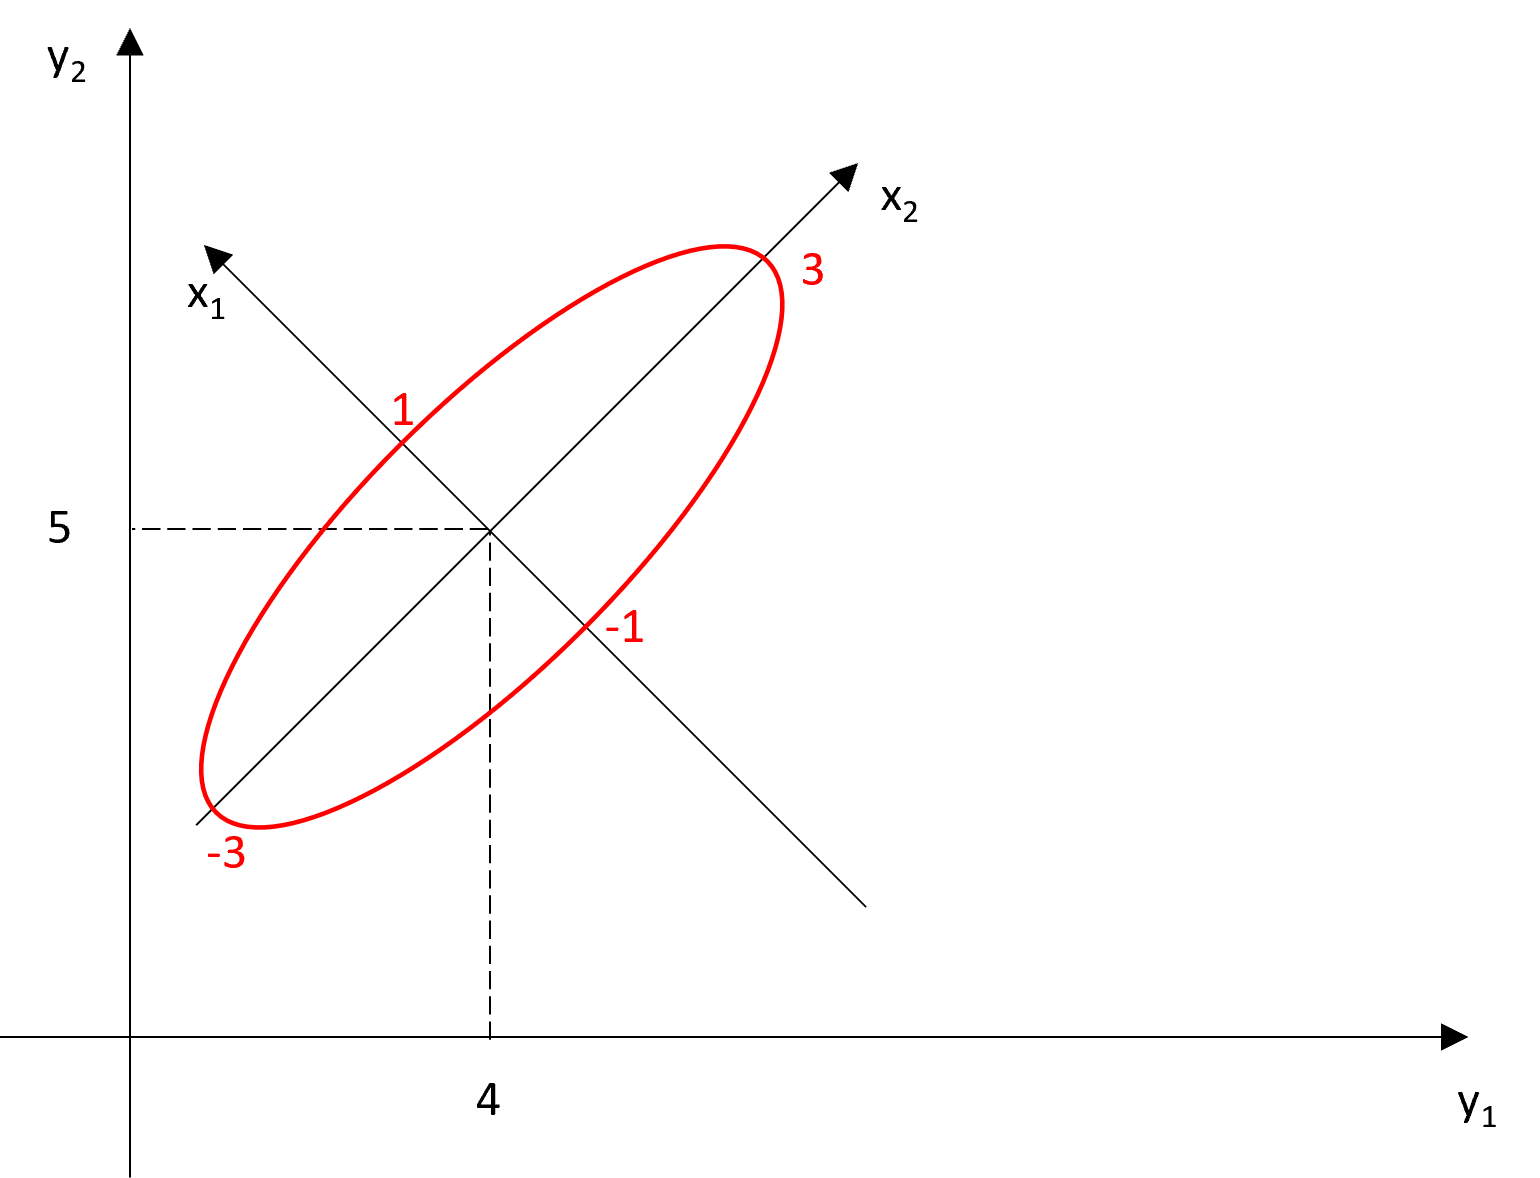
\includegraphics[scale=0.8]{B_1}
    \centering
\end{figure}
    \Exercise[number={2}]
A set of data (in \(\mathbf{R}^2\)) is described by a probability density
function of Gaussian type \(x \sim \mathcal{N}(\mu, \Sigma)\). Prove that
the contour lines of \(p(x)\), that is the locus of the points \(x\) for
which \(p(x) = constant\), describe an ellipse centered in and whose
half-axes are specified by eigenvectors and eigenvalues of \(\Sigma\).

\Answer[number={2}]
TBD
    \Exercise[number={3}]
In many physical phenomena (earthquakes, avalanches, fires, epidemics,
propagation of activity in populations of neurons) a quantity occurs that
has a statistical distribution of power-law type, i.e.:
\[
    p(x)=K_nx^{-n}
\]
with \(n>1\), , and \(x>1\), where \(K_n\) is a normalization constant
(dependent on \(n\)). 
a) Calculate the normalization function 
b) Given a dataset \(X=\{x_1,...,x_n\}\), determine an expression for the
maximum likelihood estimate of the exponent \(n\) of the distribution.

\Answer[number={3}]
To calculate the normalization function \(K_n\) it is necessary to
integrate over the proper domain (by remembering that \(x>1\)):
\begin{align*}
    \int_{1}^{+\infty}p(x)\,dx = 1 \Rightarrow
    \int_{1}^{+\infty}K_nx^{-n}\,dx
    =
    K_n\biggl[\frac{x^{1-n}}{1-n}\biggr]_{1}^{+\infty}
    =
    K_n\biggl(0-\frac{1^{1-n}}{1-n}\biggr)
    =
    1 \Rightarrow
    K_n=n-1
\end{align*}
\\
The maximum likelihood estimator for the parameter \(n\) can be found by
simply computing the derivative of the log-likelihood and equating it to
zero:
\[
    p(n|X)=\frac{p(X|n)p(n)}{p(X)} \propto p(X|n)=L(n|X)
    =
    \prod_{i=1}^{N}(n-1)x_i^{-n}
\]
\[
    \Rightarrow
    \log{L(n|X)}=N\log{(n-1)}-n\sum_{i=1}^{N}\log{x_i}
\]
\[
    \Rightarrow
    \frac{\partial{\log{L(n|X)}}}{\partial{n}}
    =
    \frac{N}{n-1}-\sum_{i=1}^{N}\log{x_i}
    =
    0
    \Rightarrow
    n-1=\frac{N}{\sum_{i=1}^{N}\log{x_i}}
\]
\[
    \Rightarrow \hat{n} = \frac{N}{\sum_{i=1}^{N}\log{x_i}} + 1
\]

    \Exercise[number={4}]
In an experiment, the measured quantities \(\{x_n, n=1...N\}\) independent of
each other, are described by a bi-exponential distribution (or Laplace
distribution), with mean \(\mu\):
\[
    p(x|\mu) = \frac{1}{Z}\exp{(-|x-\mu|)}
\]
where \(Z\) is a normalization constant (to be determined).
After having calculated \(Z\), find an expression for the maximum
likelihood estimate of \(\mu\), given the measurements.

\Answer[number={4}]
Let's define the dataset \(X=\{x_n|n=1...N\}\).
To calculate the normalization term \(Z\) it is necessary to
integrate over the proper domain:
\begin{align*}
    \int_{-\infty}^{+\infty}p(x|\mu)\,dx = 1 \Rightarrow
    \int_{-\infty}^{+\infty}\frac{1}{Z}e^{(-|x-\mu|)}\,dx
    =
    \int_{-\infty}^{\mu}\frac{1}{Z}e^{(x-\mu)}\,dx
    +
    \int_{\mu}^{+\infty}\frac{1}{Z}e^{(\mu-x)}\,dx
    =
    1
\end{align*}
\begin{align*}
    \Rightarrow
    \frac{1}{Z}\biggl[e^{x-\mu}\biggr]_{-\infty}^{\mu} - \frac{1}{Z}\biggl[e^{\mu-x}\biggr]_{\mu}^{+\infty}=1
    \Rightarrow
    Z = 1+1 = 2
\end{align*}
\\
The maximum likelihood estimator for the parameter \(\mu\) can be found by
simply computing the derivative of the log-likelihood and equating it to
zero:
\[
    p(\mu|X)=\frac{p(X|\mu)p(\mu)}{p(X)} \propto p(X|\mu)=L(\mu|X)
    =
    \prod_{i=1}^{N}\frac{1}{2}e^{-|x_i-\mu|}
\]
\[
    \Rightarrow
    \log{L(\mu|X)}=-N\log{2}-\sum_{i=1}^{N}|x_i-\mu|
\]
\[
    \Rightarrow
    \frac{\partial{\log{L(\mu|X)}}}{\partial{\mu}}
    =
    \sum_{i=1}^{N}\frac{x_i-\mu}{|x_i-\mu|}
    =
    \sum_{i=1}^{N}
    \begin{cases}
        \begin{matrix}
            1 && x_i>\mu \\ -1 && x_i<\mu
        \end{matrix}
    \end{cases}
    =
    0
\]
Therefore, the only value for the \(\mu\) parameter such that the
computed derivative of the likelihood is null is \(\hat{\mu}=median(X)\).
    \Exercise[number={5}]
From his cell, a prisoner observes through a window \(N\) stars, in positions
\(D = \{(x_i, y_i), i = 1...N\}\). He cannot see the edges of the window
because the room is totally dark apart from the stars. 
Assuming that the window is square and the positions of the stars are
independent and uniformly distributed in \(XY\) space, what can be said about
the position \((x_0, y_0)\) and the length \(L\) of the side of 
the window? [Hint: This is a probability density estimation problem.
Just write an expression for likelihood ...]

\Answer[number={5}]
First of all, it might be useful to sketch both the problem and the
probability density function:
\begin{figure}[H]
    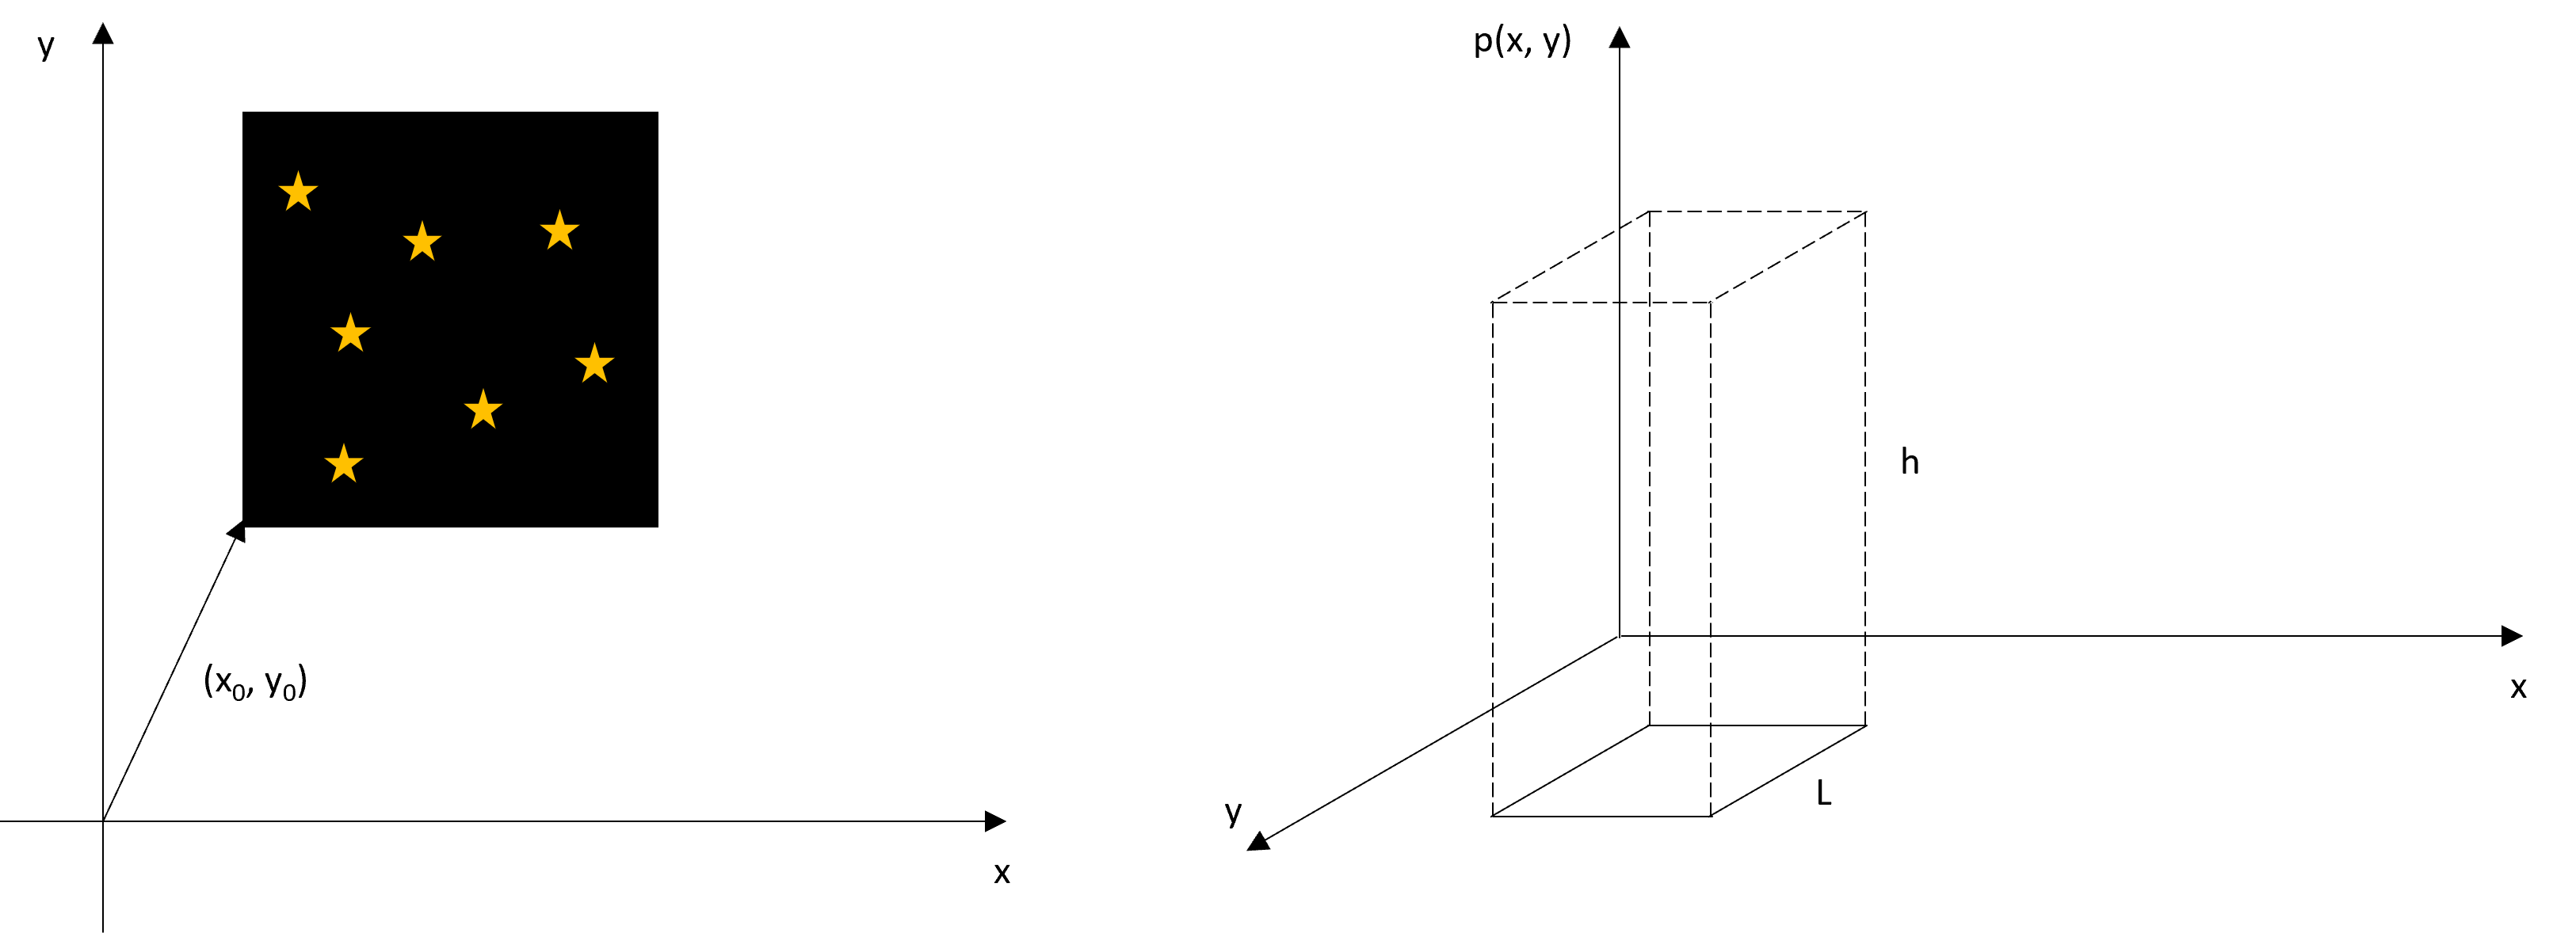
\includegraphics[scale=0.65]{B_5}
    \centering
\end{figure}
The goal of the exercise consists in finding the smallest window (thus
smallest \(L\)) such that all the \(N\) stars are visible from it.
Notice that integral of the probability density is supposed to be 1,
hence the volume of the box indicated in the right-side plot should be 1,
leading to the following:
\[
    V=1 \quad\text{and}\quad V=Ah=L^2h \Rightarrow L^2h=1 \Rightarrow h=\frac{1}{L^2}
\]
The a-posteriori probability is to be written:
\[
    p((x_0,y_0),L|D)=\frac{p(D|(x_0,y_0),L)p((x_0,y_0),L)}{p(D)}
    \propto
    p(D|(x_0,y_0),L) = L((x_0,y_0),L|D)
\]
The likelihood is evaluated as:
\[
    L((x_0,y_0),L|D) = \prod_{i=1}^{N}p((x_i,y_i)|(x_0,y_0),L)=\prod_{i=1}^{N}
    \begin{cases}
        \begin{matrix}
            h\,\Bigl(=\frac{1}{L^2}\Bigr) && (x_i, y_i)\in \text{window} \\
            0 && (x_i,y_i)\notin \text{window}
        \end{matrix}
    \end{cases}
\]
By assuming that all the \(N\) stars are seen by the window (otherwise the
likelihood product would be 0 even if just one star is not seen), it can
be said that:
\[
    L((x_0,y_0),L|D) = \biggl(\frac{1}{L^2}\biggr)^N
\]
Therefore, the likelihood is maximized when \(L\to{0}\) (as small as
possible), but still able to allow to see all the stars.
    \Exercise[number=6]
A source emits unstable particles, which decay at a distance \(x\) from
the source.
\begin{figure}[H]
    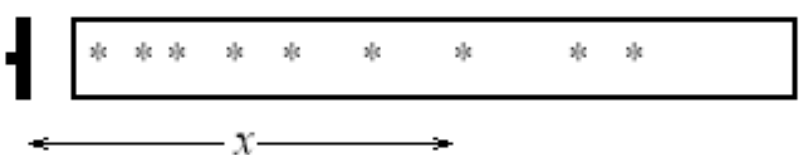
\includegraphics[scale=0.5]{B_6}
    \centering
\end{figure}
Quantity x is a real number that has an exponential distribution, with
characteristic distance \(\lambda\):
\[
    p(x|\lambda) \propto \exp{(-x/\lambda)}
\]
If \(N\) independent events \(\{ x_i, i = 1...N\}\) are observed, find an
expression for \(\lambda\). 
How does this expression change if you know that it must be
\(x > 1\) cm?

\Answer[number=6]
Let's define the dataset \(X=\{x_i|i=1...N\}\) and compute the normalization
factor \(K_{\lambda}\) by integration (notice that 0 is chosen instead
of \(-\infty\) as \(x\) is a distance and cannot be negative):
\begin{align*}
    \int_{0}^{+\infty}p(x|\mu)\,dx = 1 \Rightarrow
    \int_{0}^{+\infty}K_{\lambda}e^{-\frac{x}{\lambda}}\,dx
    =
    -K_{\lambda}\lambda\biggl[e^{-\frac{x}{\lambda}}\biggr]_{0}^{+\infty}
    =
    K_{\lambda}\lambda
    =
    1
    \Rightarrow
    K_{\lambda}
    =
    \frac{1}{\lambda}
\end{align*}
At this point, the likelihood and the log-likelihood can be written as
\[
    L(\lambda|X)=\prod_{i=1}^{N} \frac{1}{\lambda}e^{-\frac{x_i}{\lambda}}
    \Rightarrow
    \log{L(\lambda|X)}=-N\log{\lambda}-\frac{1}{\lambda}\sum_{i=1}^{N}x_i
\]
and the maximum likelihood estimator \(\hat{\lambda}\) is to be found by
deriving w.r.t. \(\lambda\) and setting the expression equal to 0:
\begin{align*}
    \frac{\partial{L(\lambda|X)}}{\partial{\lambda}}=0
    \Rightarrow
    -\frac{N}{\cancel{\lambda}}+\frac{1}{\lambda^{\cancel{2}}}\sum_{i=1}^{N}x_i=0
    \Rightarrow
    \hat{\lambda}=\frac{1}{N}\sum_{i=1}^{N}x_i
\end{align*}
\\
If \(x>1\) the lower integration bound is changed from 0 to 1, thus the
normalization factor is computed as follow:
\begin{align*}
    \int_{1}^{+\infty}p(x|\mu)\,dx = 1 \Rightarrow
    \int_{1}^{+\infty}K_{\lambda}e^{-\frac{x}{\lambda}}\,dx
    =
    -K_{\lambda}\lambda\biggl[e^{-\frac{x}{\lambda}}\biggr]_{1}^{+\infty}
    =
    K_{\lambda}\lambda e^{-\frac{1}{\lambda}}
    =
    1
    \Rightarrow
    K_{\lambda}
    =
    \frac{e^{\frac{1}{\lambda}}}{\lambda}
\end{align*}
Then, the likelihood and the log-likelihood are
\[
    L(\lambda|X)=\prod_{i=1}^{N} \frac{e^{\frac{1}{\lambda}}}{\lambda}e^{-\frac{x_i}{\lambda}}
    \Rightarrow
    \log{L(\lambda|X)}=\frac{N}{\lambda}-N\log{\lambda}-\frac{1}{\lambda}\sum_{i=1}^{N}x_i
\]
while the maximum likelihood estimator \(\hat{\lambda}\) is obtained by
deriving w.r.t. \(\lambda\) and setting the expression equal to 0:
\begin{align*}
    \frac{\partial{L(\lambda|X)}}{\partial{\lambda}}=0
    \Rightarrow
    -\frac{N}{\lambda^{\cancel{2}}}-\frac{N}{\cancel{\lambda}}+\frac{1}{\lambda^{\cancel{2}}}\sum_{i=1}^{N}x_i=0
    \Rightarrow
    -N-\lambda N+\sum_{i=1}^{N}x_i=0
    \Rightarrow
    \hat{\lambda}=\frac{1}{N}\sum_{i=1}^{N}x_i-1
\end{align*}
    \Exercise[number={7}]
A scalar variable \(x\) has a uniform probability density function:
\begin{align*}
    p(x|\theta)=
    \begin{cases}
        \begin{matrix}
            \frac{1}{\theta} && 0\ge x\ge \theta \\ 0 && \text{otherwise}
        \end{matrix}
    \end{cases}
\end{align*}
Given a specific value of \(x\), show how the function \(p(x|\theta)\)
varies with \(\theta\).\\
You have measured \(n\) independent samples \(x_1,...,x_n\).
Show that the maximum likelihood estimator of \(\theta\) is: \(\theta=\max_{k}x_k\).

\Answer[number={7}]
Let's call the specific \(x\) value \(x^*\), then the plot of the
\(p(\theta|x)\) is:
\begin{figure}[H]
    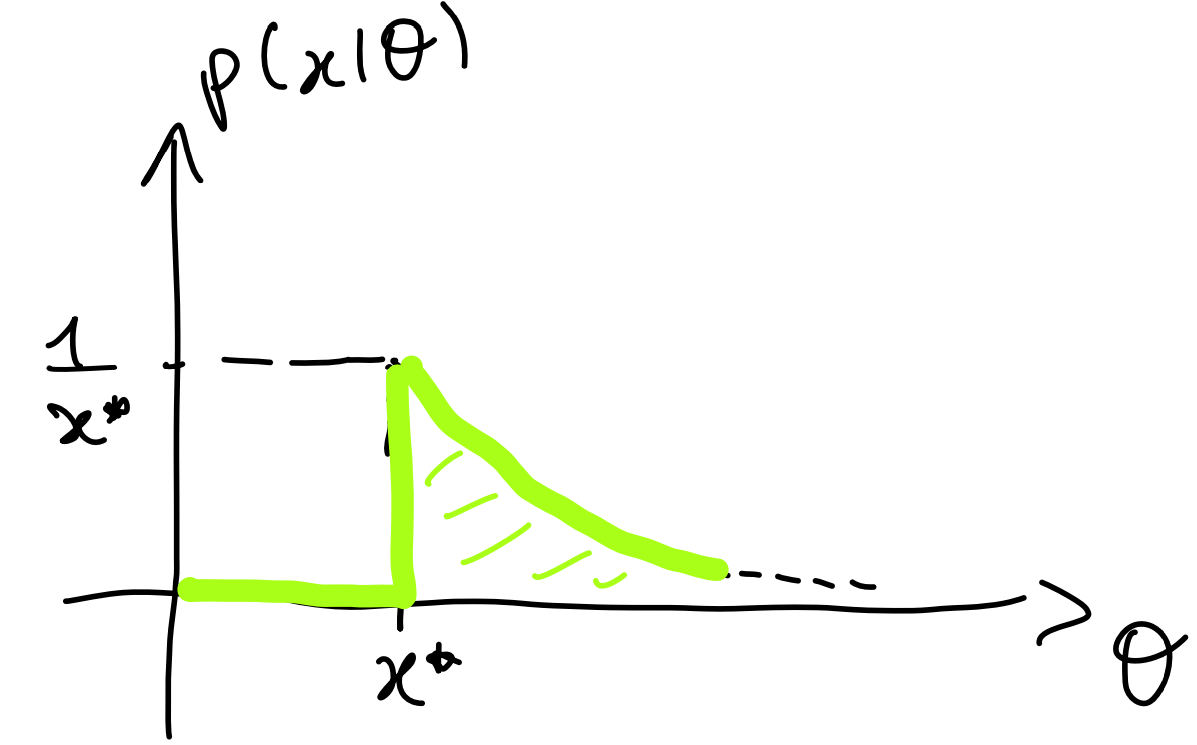
\includegraphics[scale=0.35]{B_7}
    \centering
\end{figure}
Being the dataset \(X=\{x_i|i=1,...,n\}\), the a-posteriori probability is:
\begin{align*}
    p(\theta|X)=\frac{p(X|\theta)p(\theta)}{p(X)}
    \propto
    p(X|\theta)=L(\theta|X)=\prod_{i=1}^{n}p(x_i|\theta)
\end{align*}
Thus, the likelihood is written as:
\begin{align*}
    L(\theta|X)=\prod_{i=1}^{n}\frac{1}{\theta}=\biggl(\frac{1}{\theta}\biggr)^{n}
\end{align*}
The likelihood is maximized when \(\theta\) is minimized, meaning that \(\theta\)
should be equal to \(x*\), which must be the largest of the \(x_i\) values,
otherwise at least one factor of the product is 0, leading to a null likelihood.
As a consequence, the maximum likelihood estimator \(\hat{\theta}\) can
only be \(\hat{\theta}=\max_{i}x_i\).
    \Exercise[number={8}]
A random variable \(y>0\) has the following probability density function
(Rayleigh's pdf):
\begin{align*}
    p(y)=
    \begin{cases}
        \begin{matrix}
            \frac{y}{\theta}e^{-\frac{y^2}{2\theta^2}} && y\ge0 \\ 0 && \text{otherwise}
        \end{matrix}
    \end{cases}
\end{align*}
You have \(N\) independent observations \(\{y_1,...,y_N\}\). Define a
maximum likelihood estimator for parameter \(q\). 

\Answer[number={8}]
The dataset is defined as \(Y=\{y_1,...,y_N\}\), then the a-posteriori
probability is given by the expression:
\begin{align*}
    p(\theta|Y)=\frac{p(Y|\theta)p(\theta)}{p(Y)}
    \propto
    p(Y|\theta)=L(\theta|Y)=\prod_{i=1}^{N}p(y_i|\theta)
\end{align*}
Notice that it is necessary to assume always \(y_i\ge0\), otherwise the
product results equal to 0 and the likelihood wouldn't be maximized. \\
Said so, the likelihood is expressed as
\begin{align*}
    L(\theta|Y)=\prod_{i=1}^{N}\frac{y_i}{\theta}e^{-\frac{y_i^2}{2\theta^2}}
    \Rightarrow
    \log{L(\theta|Y)}=\sum_{i=1}^{N}\log{y_i} - 2N\log{\theta} - \frac{1}{2\theta^2}\sum_{i=1}^{N}y_i^2
\end{align*}
and the maximum likelihood estimator \(\hat{\theta}\) is given by the derivative
set to 0:
\begin{align*}
    \frac{\partial{\log{L(\theta|Y)}}}{\partial{\theta}}=0
    \Rightarrow
    -\frac{2N}{\theta} + \frac{1}{\theta^3}\sum_{i=1}^{N}y_i^2=0
    \Rightarrow
    -2N\theta^2 + \sum_{i=1}^{N}y_i^2=0
    \Rightarrow
    \hat{\theta}=\pm\sqrt{\frac{1}{2N}\sum_{i=1}^{N}y_i^2}
\end{align*}
    \Exercise[number={9}]
Let \(\bar{x}\) be a binary vector (i.e. each element may be either 0 or 1), with a
multivariate Bernoulli distribution:
\[
    p(\bar{x}|\bar{\theta})=\prod_{i=1}^{d}\theta_i^{x_i}(1-\theta_i)^{1-x_i}
\]
where \(\bar{\theta}=[\theta_1,...,\theta_d]^T\) is a vector of parameters,
where \(\theta_i = p(x_i=1)\). Given \(N\) independent measures
\(\bigl\{ \bar{x}_n, n=1,...,N \bigr\}\) develop a maximum likelihood
estimator of \(\bar{\theta}\).

\Answer[number={9}]
Let the dataset be \(X=\{x_n, n=1,...,N\}\), then the posterior probability
and the likelihood are
\begin{align*}
    p(\bar{\theta}|X) \propto p(X|\bar{\theta})
    =
    L(\bar{\theta}|X) = \prod_{n=1}^{N}L(\bar{\theta}|x_n)
    =
    \prod_{n=1}^{N} \prod_{i=1}^{d} \theta_i^{x_{ni}}(1-\theta_i)^{(1-x_{ni})}
\end{align*}
since the data sample \(x_n\) is \(d\)-dimensional.
Consequently, the log-likelihood results as:
\begin{align*}
    \log{L(\bar{\theta}|X)}
    &=
    \sum_{n=1}^{N}\sum_{i=1}^{d} \biggl[x_{ni}\log{\theta_i}+(1-x_{ni})\log{(1-\theta_i)}\biggr] \\  
    &=
    \sum_{n=1}^{N}\biggl[\sum_{i=1}^{d}x_{ni}\log{\theta_i}+\sum_{i=1}^{d}(1-x_{ni})\log{(1-\theta_i)}\biggr] \\
    &=
    \sum_{n=1}^{N}
    \begin{cases}
        \begin{matrix}
            \sum_{i=1}^{d}\log{\theta_i} && x_{ni} = 1 \\
            \sum_{i=1}^{d}\log{(1-\theta_i)} && x_{ni} = 0
        \end{matrix}
    \end{cases}
\end{align*}
Notice that \(\theta_i\) is the probability such that \(x_{ni}=1\), which is
a binary variable, assuming exclusively 0 or 1 values. As a consequence,
\(\theta_i\) lays in the interval between 0 and 1, meaning that the log-likelihood
is always negative: \(-\infty<\log{\theta_i}<0\). The same reasoning
works in an opposite way for the \(\log{(1-\theta_i)}\) case. \\
Said so, the likelihood is maximum when all the addends are null, otherwise
some negative factors would be added to the sum, obtaining an overall value
lower than 0. This makes sense, as the maximum posterior probability
(proportional to the likelihood) is obtained when the outcome of a random event
is fully known, implying that the related probability is either
\(\hat{\theta_i}=0\) or \(\hat{\theta_i}=1\).
    \Exercise[number={10}]
In an experiment, real and positive quantities \(x\) are measured, described
by an exponential distribution:
\[
    p(x|\lambda) \propto \lambda^{-x}
\]
where \(\lambda>0\) is a parameter. \\
a. Determine the normalization factor \(K\). [Hint: should be
\(K\int_0^{+\infty}\lambda^{-x}\,dx = 1\)
] \\
b. Given a \(x\), analyze the function \(L(\lambda)=p(x|\lambda)\) and
display it in a Cartesian graph. \\
c. Given \(N\) independent measures \(\bigl\{ x_n, n=1,...,N \bigr\}\),
derive a maximum likelihood estimator for \(\lambda\).

\Answer[number={10}]
a. To find the normalization term \(K\), the integral between 0 and \(+\infty\) is to
be calculated:
\begin{align*}
    \int_{0}^{+\infty}Kp(x|\lambda)\,dx = 1
    \Rightarrow
    K\int_{0}^{+\infty}\lambda^{-x}\,dx
    =
    K\biggl[\frac{\lambda^{-x}}{\log{\lambda}}\biggr]_{0}^{+\infty}
\end{align*}
Notice that the integral is undefined as long as \(\lambda \le 1\), thus
a new condition is to be set, in particular \(\lambda > 1\), leading
to the integral expression below:
\begin{align*}
    \int_{1}^{+\infty}Kp(x|\lambda)\,dx = 1
    \Rightarrow
    K\int_{1}^{+\infty}\lambda^{-x}\,dx
    =
    K\biggl[\frac{\lambda^{-x}}{\log{\lambda}}\biggr]_{1}^{+\infty}
    =
    \frac{K}{\log{\lambda}}=1
    \Rightarrow
    K=\log{\lambda}
\end{align*}
b. The likelihood \(L(\lambda|x)=\log{(\lambda)}\lambda^{-x}\). Given the
preivous considerations, the domain is \(\lambda>1\) and the likelihood
has a positive sign in the whole domain. The asymptotes are computed as:
\begin{align*}
    \lim_{\lambda\to{1^+}}\log{(\lambda)}\lambda^{-x} = 0 \\
    \lim_{\lambda\to{+\infty}}\log{(\lambda)}\lambda^{-x} = 0
\end{align*}
Let's compute the derivative of \(L(\lambda)\) and study its sign:
\begin{align*}
    \frac{d\,L(\lambda)}{d\,\lambda}
    =
    \frac{d\,\log{(\lambda)}\lambda^{-x}}{d\,\lambda}
    =
    \frac{\lambda^{-x}}{\lambda}+\log{(\lambda)}(-x)\lambda^{-(x+1)}
    =
    \lambda^{-(x+1)}\bigl[1-x\log{\lambda}\bigr]
\end{align*}
\begin{align*}
    \cancel{\lambda^{-(x+1)}}\bigl[1-x\log{\lambda}\bigr] > 0
    \Longleftrightarrow
    1-x\log{\lambda} > 0
    \Longleftrightarrow
    \log{\lambda} < \frac{1}{x}
    \Longleftrightarrow
    \lambda < e^{\frac{1}{x}}
\end{align*}
Therefore, \(\lambda = e^{\frac{1}{x}}\) is the global maximum for the
likelihood function in the given domain \(\lambda>1\). \\
The likelihood as function of \(\lambda\) exhibits the following plot:
\begin{figure}[H]
    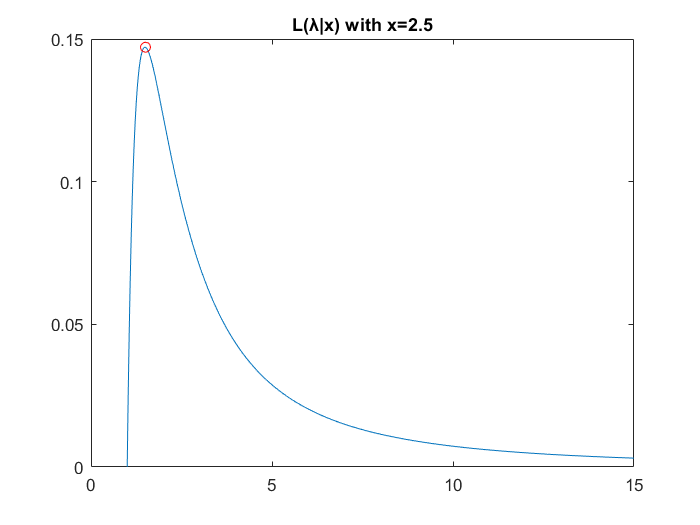
\includegraphics[scale=0.65]{B_10}
    \centering
\end{figure}
c. Let's define a dataset \(X=\{x_n, n=1,...,N\}\), then the likelihood
can be written as \(L(\lambda|X)=\prod_{i=1}^{N}\log{(\lambda)}\lambda^{-x_i}\).
Thus, the log-likelihood is:
\begin{align*}
    \log{L(\lambda|X)}=\sum_{i=1}^{N}\log{(\log{\lambda})}-\sum_{i=1}^{N}x_i \log{\lambda}
    =
    N\log{(\log{\lambda})} - \log{\lambda}\sum_{i=1}^{N}x_i
\end{align*}
By taking the derivative of the log-likelihood and setting it to zero, the
maximum likelihood estimator \(\hat{\lambda}\) can be obtained:
\begin{align*}
    \frac{\partial{\log{L(\lambda|X)}}}{\partial{\lambda}}=0
    &\Rightarrow
    \frac{N}{\log{\lambda}}\frac{1}{\lambda}-\frac{1}{\lambda}\sum_{i=1}^{N}x_i=0 \\
    &\Rightarrow
    \frac{1}{\lambda}\biggl[\frac{N}{\log{\lambda}} - \sum_{i=1}^{N}x_i\biggr]=0 \\
    &\Rightarrow
    \hat{\lambda_1}\to +\infty,
    \quad\quad
    \frac{N}{\sum_{i=1}^{N}} = \log{\lambda} \Rightarrow \hat{\lambda_2}=e^{\frac{N}{\sum_{i=1}^{N}x_i}}=e^{\frac{1}{mean(X)}}
\end{align*}
Notice how \(\hat{\lambda_2}\) has a form consistent with the global maximum
obtained before for a single value \(x\).
    \Exercise[number={11}]
A vector y of measures is described by the factorial model \((\Lambda, \Psi)\):
\[
    y_d=\sum_{k=1}^{K} \Lambda_{dk}x_k+\epsilon_d
\]
in terms of \(K\) orthogonal factors \(x_k\sim \mathcal{N}(0,1)\) and a Gaussian
noise \(\epsilon_d \sim \mathcal{N}(0, \Psi_{dd})\) with a diagonal \(\Psi_{dd}\).
Assume that the \(i\)-th element of \(y\) is scaled by a factor \(h\), i.e.
\(y_i'=h y_i\). How does the factorial model (and the factors \(x_k\) ) change
for the scaled vector \(y'\)?

\Answer[number={11}]
First of all, let's point out that
\(y=\Lambda x + \epsilon = \sum_{i=1}^{K}(\lambda_i x_i)+\epsilon\),
\(x_i\sim\mathcal{N}(0, 1) \Rightarrow x\sim\mathcal{N}(0, I)\),
\(\epsilon\sim\mathcal{N}(0, \Psi)\), and, consequently,
\(y\sim\mathcal{N}(0, \Sigma)\), where
\begin{align*}
    \Sigma
    &=E\{\bigl[y-E\{y\}\bigr]\bigr[y-E\{y\}\bigr]^T\}
    =E\{yy^T\}
    =E\{\Lambda x x^T \Lambda^T\} + E\{\epsilon\epsilon^T\}\\
    &=E\{\Lambda I \Lambda^T\} + \Psi
    =E\{\Lambda\Lambda^T\} + \Psi
    =\Lambda\Lambda^T + \Psi
\end{align*}
Now, let's introduce a homogeneous transformation \(H\) to scale the
vector \(y\), leading to:
\begin{align*}
    y'=Hy=H\Lambda x + H\epsilon \Rightarrow y'=\Lambda'x + \epsilon'
\end{align*}
Notice that a scaling matrix must have the determinant different from 1
(otherwise no scaling) and must be diagonal, otherwise a rotation occurs. \\
Let's try to determine \(\Psi'\) by exploiting the
definition of variance as expected value:
\begin{align*}
    \Psi'
    =E\{\bigl[\epsilon'-E\{\epsilon'\}\bigr]\bigr[\epsilon'-E\{\epsilon'\}\bigr]^T\}
    =E\{\epsilon'\epsilon'^T\}
    =E\{H\epsilon\epsilon^T H^T\}
    =HE\{\epsilon\epsilon^T\}H^T
    =H\Psi H^T
\end{align*}
Therefore, \(\epsilon'\sim\mathcal{N}(0, \Psi')\). Similarly,
\begin{align*}
    \Sigma'
    &=E\{\bigl[y'-E\{y'\}\bigr]\bigr[y'-E\{y'\}\bigr]^T\}
    =E\{y'y'^T\}
    =E\{Hyy^T H^T\}
    =HE\{yy^T\}H^T\\
    &=H\Sigma H^T
    =H(\Lambda\Lambda^T + \Psi)H^T
    =H\Lambda\Lambda^T H^T + \Psi'
    =\Lambda'\Lambda'^T + \Psi'
\end{align*}
According to the definition of factor analysis, the eigenvalue
decomposition of the \(y\) covariance matrix is
\(\Sigma=\Lambda I \Lambda^T\), while the decomposition of the \(y'\)
covariance matrix is \(\Sigma'=H\Lambda I\Lambda^T H^T = \Lambda'I\Lambda'^T\).
Notice that \(\Lambda'\) has no particular constraints in FA, therefore scaling
\(\Lambda\) by matrix \(H\) doesn't go against the FA assumptions.
The same can be said for \(\Psi'\), which must be a diagonal matrix, but the
scaling matrix \(H\) is diagonal itself, as previously said, thus multiplying
a diagonal \(\Psi\) by another diagonal \(H\) produces once again a diagonal
matrix \(\Psi'\).\\
Said so, it is clear that the assumptions necessary for the Factor Analysis
are not violated and the only element producing a difference between \(y\)
and \(y'\) w.r.t. \(x\) is the scaling matrix \(H\), thus the same
components \(x\) are obtained, making it invariant.
    \Exercise[number={12}]
A quantity \(\mu\) is measured through \(N\) independent measurement channels.
Every channel introduces an additive Gaussian noise \(\eta_i\), \(i=1,...,N\),
with zero mean and variance \(\sigma_i^2\). Define a maximum likelihood
estimator for \(\mu\), given the measures \(y_i = \mu + \eta_i\) from each
channel.

\Answer[number={12}]
The quantity \(\mu\) represents the true value, while \(y\) is a vector of
\(N\) observations of the true value \(\mu\) with a variable noise
\(\eta\sim\mathcal{N}(0, \Sigma)\), being \(\Sigma\) a diagonal covariance
matrix.\\
The likelihood can be expressed as:
\begin{align*}
    L(\mu|y)=\prod_{i=1}^{N}L(\mu|y_i)=\prod_{i=1}^{N}\frac{1}{\sqrt{2\pi\sigma_i^2}}e^{\frac{1}{2\sigma_i^2}(y_i-\mu)^2}
\end{align*}
Consequently, the log-likelihood becomes:
\begin{align*}
    \log{L(\mu|y)}
    =
    \sum_{i=1}^{N}\biggl[-\frac{1}{2}\log{(2\pi\sigma_i^2)}-\frac{1}{2\sigma_i^2}(y_i-\mu)^2\biggr]
\end{align*}
The maximum likelihood estimator \(\hat{\mu}\) is obtained by deriving the
log-likelihood expression and setting it to 0:
\begin{align*}
    \frac{\partial{L(\mu|y)}}{\partial{\mu}}=0
    \Rightarrow
    \sum_{i=0}^{N}\cancel{-}\cancel{2}\frac{1}{\cancel{2}\sigma_i^2}(y_i-\mu)=0
    \Rightarrow
    \sum_{i=1}^{N}\frac{y_i}{\sigma_i^2}=\mu\sum_{i=1}^{N}\frac{1}{\sigma_i^2}
    \Rightarrow
    \hat{\mu}=\frac{\sum_{i=1}^{N}\frac{y_i}{\sigma_i^2}}{\sum_{i=1}^{N}\frac{1}{\sigma_i^2}}
\end{align*}
    \Exercise[number={14}]
A scalar random variable \(x\) is described by a mixture of two Gaussians with the
same variance \(\sigma^2\) and different means, \(\mu_1\) and \(\mu_2\):
\[
    p(x|\mu_1,\mu_2,\sigma^2)=\sum_{i=1}^2\pi_i\frac{1}{\sqrt{2\pi\sigma^2}}e^{-\frac{1}{2}(x-\mu_i)^2}
\]
and where \(\pi_1=\pi_2=0.5\). Consider a dataset \(\{x_n,n=1,...,N\}\) indipendently
drawn from this distribution. Let \(S_n\) be the (unknown) class of the \(n\)-th
sample, \(x_n\) (i.e. the "hidden" source which actually generated \(x_n\)).
Prove that the posterior probabilities of class \(S_n\), given \(x_n\), have the
following form:
\[
    Pr(S_n=1|x_n,\mu_1,\mu_2,\sigma^2)=\frac{1}{1+e^{-(w_0+wx_n)}}
    \quad\text{and}\quad
    Pr(S_n=2|x_n,\mu_1,\mu_2,\sigma^2)=\frac{1}{1+e^{+(w_0+wx_n)}}
\]

\Answer[number={14}]
Let's recall the general formula for the responsibility of the Gaussian component
\(k\) for a generic data point \(x_n\):
\begin{align*}
    r_k=Pr(S_n=k|x_n,\mu,\Sigma)
    =\frac{\pi_k p(x_n|\mu_k,\Sigma_k)}{\sum_{i=1}^K\pi_i p(x_n|\mu_i,\Sigma_i)}
\end{align*}
For the given case, the responsibility for cluster 1 is:
\begin{align*}
    Pr(S_n=1|x_n,\mu_1,\mu_2,\sigma^2)
    &=\frac{\pi_1 p(x_n|\mu_1,\sigma^2)}{\sum_{i=1}^2\pi_i p(x_n|\mu_i,\sigma^2)}
    =\frac{\cancel{\frac{1}{2}\frac{1}{\sqrt{2\pi\sigma^2}}}e^{-\frac{1}{2\sigma^2}(x_n-\mu_1)^2}}{\cancel{\frac{1}{2}\frac{1}{\sqrt{2\pi\sigma^2}}}e^{-\frac{1}{2\sigma^2}(x_n-\mu_1)^2}+\cancel{\frac{1}{2}\frac{1}{\sqrt{2\pi\sigma^2}}}e^{-\frac{1}{2\sigma^2}(x_n-\mu_2)^2}}\\
    &=\frac{1}{1+e^{-\frac{1}{2\sigma^2}(x_n-\mu_2)^2+\frac{1}{2\sigma^2}(x_n-\mu_1)^2}}
    =\frac{1}{1+e^{-\frac{1}{2\sigma^2}(\cancel{x_n^2}+\mu_2^2-2x_n\mu_2-\cancel{x_n^2}-\mu_1^2+2x_n\mu_1)}}\\
    &=\frac{1}{1+e^{-\bigl(\frac{\mu_2^2-\mu_1^2}{2\sigma^2}+\frac{\mu_1-\mu_2}{\sigma^2}x_n\bigr)}}
    =\frac{1}{1+e^{-(w_0+wx_n)}}
\end{align*}
Similarly, the responsibility for cluster 2 is:
\begin{align*}
    Pr(S_n=2|x_n,\mu_1,\mu_2,\sigma^2)
    &=\frac{\pi_2 p(x_n|\mu_2,\sigma^2)}{\sum_{i=1}^2\pi_i p(x_n|\mu_i,\sigma^2)}
    =\frac{\cancel{\frac{1}{2}\frac{1}{\sqrt{2\pi\sigma^2}}}e^{-\frac{1}{2\sigma^2}(x_n-\mu_2)^2}}{\cancel{\frac{1}{2}\frac{1}{\sqrt{2\pi\sigma^2}}}e^{-\frac{1}{2\sigma^2}(x_n-\mu_1)^2}+\cancel{\frac{1}{2}\frac{1}{\sqrt{2\pi\sigma^2}}}e^{-\frac{1}{2\sigma^2}(x_n-\mu_2)^2}}\\
    &=\frac{1}{1+e^{-\frac{1}{2\sigma^2}(x_n-\mu_1)^2+\frac{1}{2\sigma^2}(x_n-\mu_2)^2}}
    =\frac{1}{1+e^{-\frac{1}{2\sigma^2}(\cancel{x_n^2}+\mu_1^2-2x_n\mu_1-\cancel{x_n^2}-\mu_2^2+2x_n\mu_2)}}\\
    &=\frac{1}{1+e^{+\bigl(\frac{\mu_2^2-\mu_1^2}{2\sigma^2}+\frac{\mu_1-\mu_2}{\sigma^2}x_n\bigr)}}
    =\frac{1}{1+e^{+(w_0+wx_n)}}
\end{align*}
Notice that:
\begin{align*}
    w_0=\frac{\mu_2^2-\mu_1^2}{2\sigma^2}
    \quad\text{and}\quad
    w=\frac{\mu_1-\mu_2}{\sigma^2}
\end{align*}
\end{ExerciseList}
\newpage

\section*{Unit C - Pattern analysis and decision theory}
\graphicspath{ {./unit_C/images/} }
\begin{ExerciseList}
    \Exercise[number={1}]
A variable \(x\) in \(\mathbf{R}\) (scalar) is emitted by two possible sources,
\(w_1\), \(w_2\) with probability \(Pr(w_1)=Pr(w_2)=0.5\). 
We intend to design a Bayes classifier that assigns the correct class to each
observed \(x\). If the \(p(x|w_i)\) both have a Gaussian distribution, with
mean \(\mu_i\) and different variances \(\sigma_i^2\), determine the
boundaries of the decision regions as \(h=\sigma_2^2 / \sigma_1^2\)
varies.

\Answer[number={1}]
The boundaries of a binary classifier can be studied by computing the
sign of \(z(x)\), with \(z\) being the exponent of the sigmoid function, in
particular the decision boundaries are given by \(z(x)=0\).
\begin{align*}
    z(x)
    &=\log{\frac{p(x|w_1)}{p(x|w_2)}} + \log{\frac{Pr(w_1)}{Pr(w_2)}}
    =\log{p(x|w_1)}-\log{p(x|w_2)}+\cancel{\log{\frac{0.5}{0.5}}}\\
    &=-\frac{1}{2}\log{(2\pi\sigma_1^2)}-\frac{1}{2\sigma_1^2}(x-\mu_1)^2+\frac{1}{2}\log{(2\pi\sigma_2^2)}+\frac{1}{2\sigma_2^2}(x-\mu_2)^2\\
    &=\frac{1}{2}\log{\biggl(\frac{\cancel{2\pi}\sigma_2^2}{\cancel{2\pi}\sigma_1^2}\biggr)}+\frac{1}{2}\biggl(\frac{x^2+\mu_2^2-2\mu_2x}{\sigma_2^2}-\frac{x^2+\mu_1^2-2\mu_1x}{\sigma_1^2}\biggr)
\end{align*}
\begin{align*}
    z(x)=0 \Longleftrightarrow \cancel{\frac{1}{2}}\log{\biggl(\frac{\sigma_2^2}{\sigma_1^2}\biggr)}+\cancel{\frac{1}{2}}\biggl(\frac{x^2+\mu_2^2-2\mu_2x}{\sigma_2^2}-\frac{x^2+\mu_1^2-2\mu_1x}{\sigma_1^2}\biggr)=0
\end{align*}
\begin{align*}
    \Rightarrow
    \biggl(\frac{1}{\sigma_2^2}-\frac{1}{\sigma_1^2}\biggr)x^2+
    2\biggl(\frac{\mu_1}{\sigma_1^2}-\frac{\mu_2}{\sigma_2^2}\biggr)x+
    \biggl(\frac{\mu_2^2}{\sigma_2^2}-\frac{\mu_1^2}{\sigma_1^2}\biggr)+
    \log{\biggl(\frac{\sigma_2^2}{\sigma_1^2}\biggr)}
    =0
\end{align*}
Notice that, given this 2nd order polynomial and by assuming \(\mu_1<\mu_2\),
three cases are possible:\\
\begin{enumerate}
    \item \(h=1\Rightarrow\sigma_1^2=\sigma_2^2\): in this case the 2nd order term
    goes to 0, meaning that a single point dividing the two classes \(w_1\) and \(w_2\)
    is individuated, as in the piture below:
    \begin{figure}[H]
        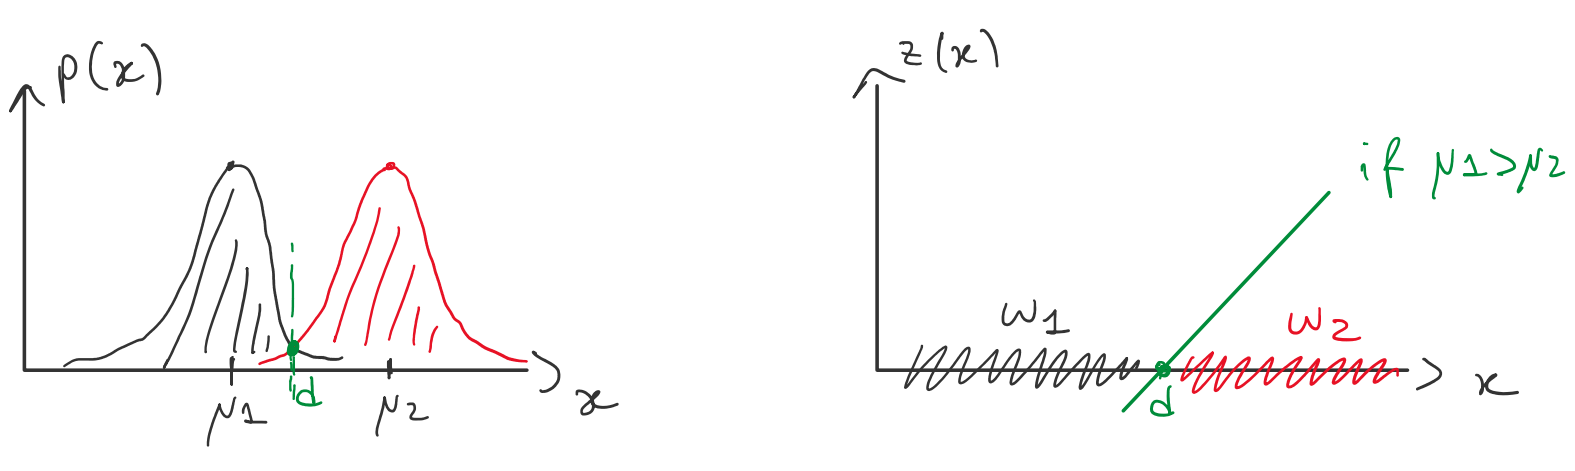
\includegraphics[scale=0.45]{C_1_1}
        \centering
    \end{figure}
    \item \(h>1\Rightarrow\sigma_1^2<\sigma_2^2\): the Gaussian distribution of \(w_1\)
    has a smaller variance, thus it is steeper, while \(w_2\) is wider, the polynomial \(z(x)\)
    is of 2nd order and the sign in front of \(x^2\) is negative, thus the
    positive portion of the parabula indicates the interval on the variable \(x\)
    which would select the class \(w_1\).
    \begin{figure}[H]
        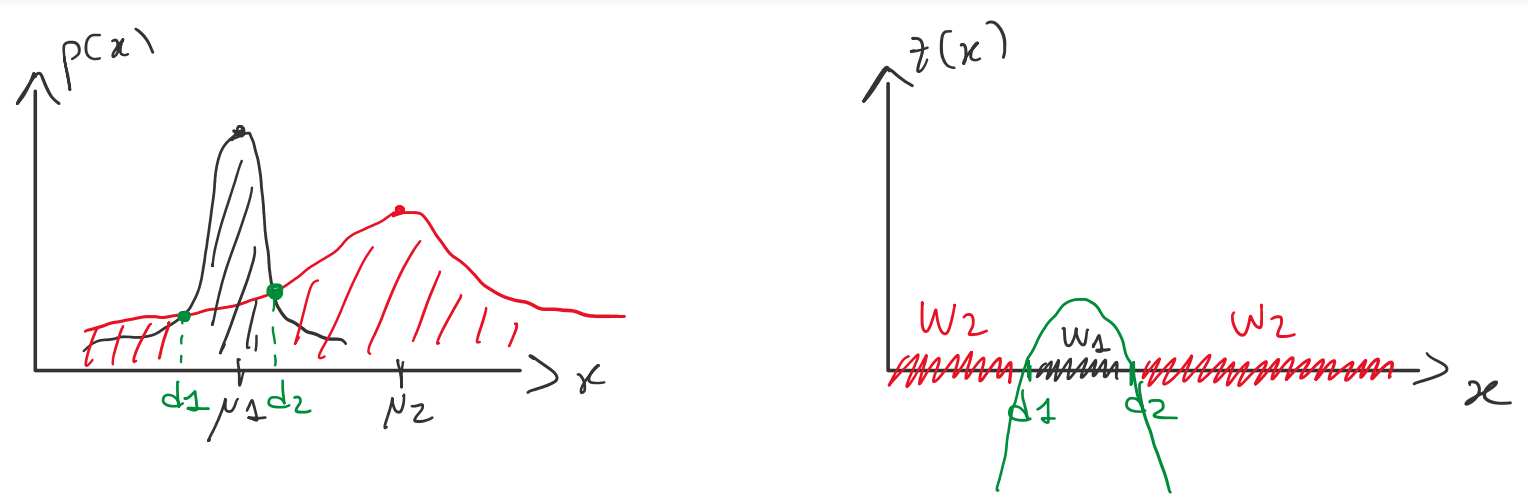
\includegraphics[scale=0.45]{C_1_2}
        \centering
    \end{figure}
    \item \(h<1\Rightarrow\sigma_1^2>\sigma_2^2\): the Gaussian distribution of \(w_1\)
    has a larger variance, thus it is wider, while \(w_2\) is steeper, the polynomial \(z(x)\)
    is of 2nd order and the sign in front of \(x^2\) is positive, thus the
    negative portion of the parabula indicates the interval on the variable \(x\)
    which would select the class \(w_2\).
    \begin{figure}[H]
        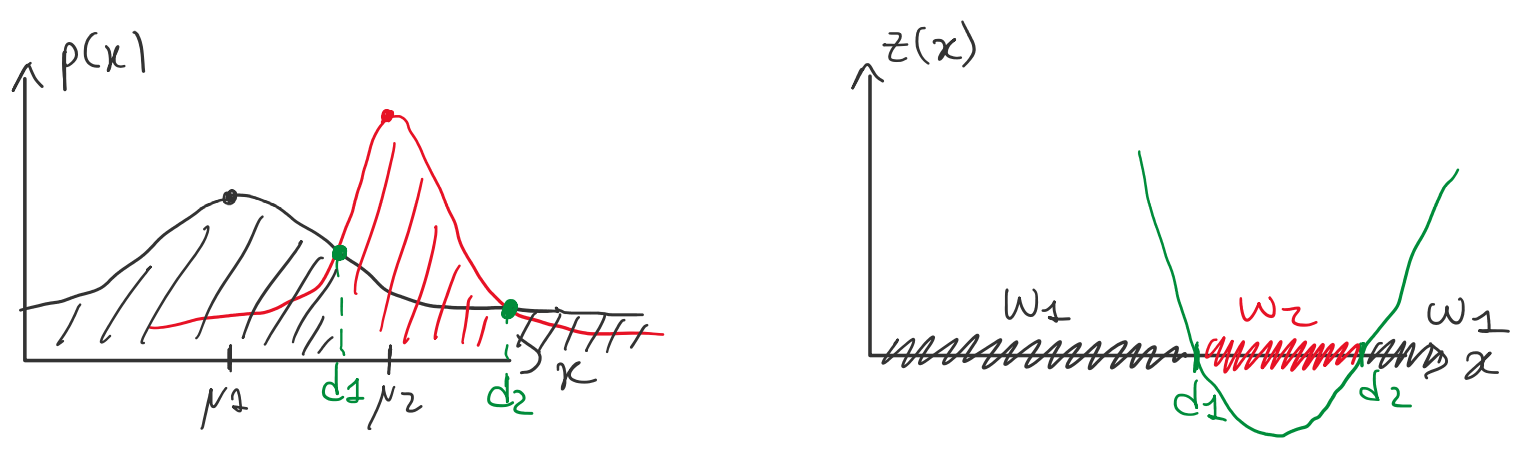
\includegraphics[scale=0.45]{C_1_3}
        \centering
    \end{figure}
  \end{enumerate}
    \Exercise[number={2}]
A variable \(x\) in \(\mathbf{R}^2\) is emitted by two possible sources,
\(w_1\) and \(w_2\), of probability \(Pr(w_1)=p\) and \(Pr(w_2)=1-p\). 
We intend to design a Bayes classifier that assigns the correct class to each
observed \(x\). If the \(p(x|w_i)\) both have a Gaussian distribution, with
mean \(\mu_i\) and variance \(I\sigma^2\) (same for the two classes),
draw the boundaries of the decision regions as \(p\) varies.

\Answer[number={2}]
The boundaries of a binary classifier can be studied by computing the
sign of \(z(x)\), with \(z\) being the exponent of the sigmoid function, in
particular the decision boundaries are given by \(z(x)=0\).
\begin{align*}
    z(x)
    &=\log{\frac{p(x|w_1)}{p(x|w_2)}} + \log{\frac{Pr(w_1)}{Pr(w_2)}}
    =\log{p(x|w_1)}-\log{p(x|w_2)}+\log{\frac{p}{1-p}}\\
    &=-\cancel{\log{\frac{2\pi}{2\pi}}}-\cancel{\frac{1}{2}\log{\frac{|\Sigma_1|}{|\Sigma_2|}}}-\frac{1}{2\sigma^2}\bigl[(x-\mu_1)^T(x-\mu_1)-(x-\mu_2)^T(x-\mu_2)\bigr]+\log{\frac{p}{1-p}}\\
    &=-\frac{1}{2\sigma^2}\bigl[(\mu_1^T\mu_1-\mu_2^T\mu_2)-2(\mu_1-\mu_2)^Tx\bigr]+\log{\frac{p}{1-p}}\\
    &=-\frac{1}{2\sigma^2}\bigl[(\mu_1-\mu_2)^T(\mu_1+\mu_2-2x)\bigr]+\log{\frac{p}{1-p}}\\
    &=\frac{1}{\sigma^2}\biggl[(\mu_1-\mu_2)^T(x-\frac{\mu_1-\mu_2}{2})\biggr]+\log{\frac{p}{1-p}}
\end{align*}
\begin{align*}
    z(x)=0 \Longleftrightarrow \frac{1}{\sigma^2}\biggl[(\mu_1-\mu_2)^T(x-\frac{\mu_1-\mu_2}{2})\biggr]+\log{\frac{p}{1-p}}=0
\end{align*}
Notice that the first part of the equation is derived from
\(\log{\frac{p(x|w_1)}{p(x|w_2)}}\) and it must be zero on the decision
boundary, as both the likelihoods must be equal to 0.5. Moreover, it represents
a scalar product between two vectors: the first one represents the line
connecting \(\mu_1\) and \(\mu_2\), the second one is the line connecting
a generic \(x\) to the middle point of the line connecting the two means.
However, due to the presence of the right-side term \(\log{\frac{p}{1-p}}\),
the intersection point with the \(\mu_1-\mu_2\) line is moved from
the middle point towards the class center having a lower probability \(Pr(w_i)\),
making the area on the plane accounting for that lower probability class smaller.
In the 3D space, the equation \(z(x)=(\mu_1-\mu_2)^T(x-\frac{\mu_1-\mu_2}{2})\)
represents a hyperplane (in this case a plane), with an offset
\(\log{\frac{p}{1-p}}\), affecting where the plane intersects the plane
generated by \(x_1\) and \(x_2\) components.
Hence, three cases are possible:
\begin{enumerate}
    \item \(Pr(w_1)=Pr(w_2)=0.5\Rightarrow\log{\frac{p}{1-p}}=0\):
    the scalar product between the aforementioned vectors is null, implying
    that the two vectors must be perpendicular. Consequently, the following
    image, representing the decision boundaries, can be drawn:
    \begin{figure}[H]
        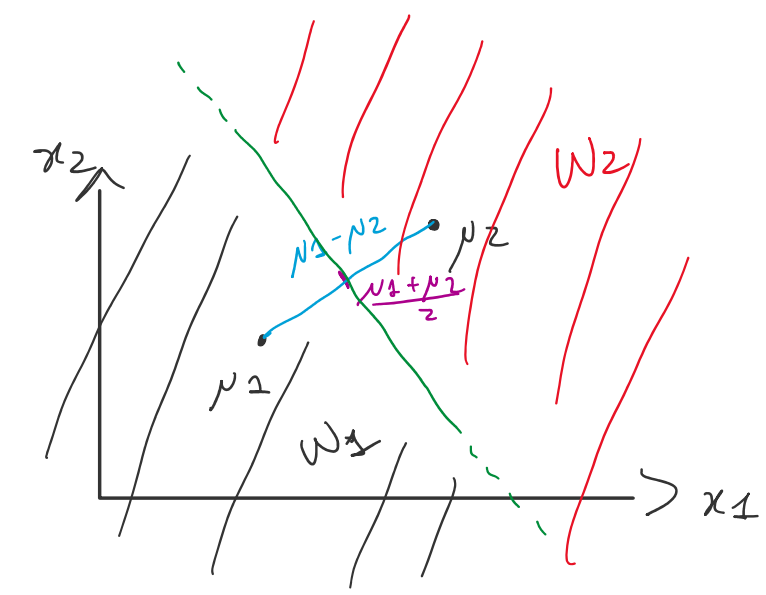
\includegraphics[scale=0.45]{C_2}
        \centering
    \end{figure}
    \item \(Pr(w_1)=p>Pr(w_2)=1-p\Rightarrow\log{\frac{p}{1-p}}>0\):
    the scalar product must once again be zero, however, the factor
    \(\log{\frac{p}{1-p}}\) implies a translation of the decision line
    toward the \(\mu_2\) mean. This is consistent with a translation
    toward the negative side of the sigmoid, since there is a bias
    toward the selection of class \(w_1\) (\(Pr(w_1)>0.5\)).
    \item \(Pr(w_1)=p<Pr(w_2)=1-p\Rightarrow\log{\frac{p}{1-p}}<0\):
    the scalar product must once again be zero, however, the factor
    \(\log{\frac{p}{1-p}}\) implies a translation of the decision line
    toward the \(\mu_1\) mean. This is consistent with a translation
    toward the positive side of the sigmoid, since there is a bias
    toward the selection of class \(w_2\) (\(Pr(w_2)>0.5\)).
  \end{enumerate}
    \Exercise[number={3}]
A variable \(x\) in \(\mathbf{R}^2\) is emitted by two possible sources,
\(w_1\) and \(w_2\), with equal a priori probability \(Pr(w_1)=Pr(w_2)\). 
We want to design a Bayes classifier that assigns the correct class to each
observed \(x\). If the \(p(x|w_i)\) both have a Gaussian distribution, with
mean \(\mu_i\) and variance \(I\sigma_i^2\) (with \(\sigma_1>\sigma_2\)),
show that the boundary of the decision regions for the classifier is a circle.
Then determine the radius and the coordinates of the center.

\Answer[number={3}]
The boundaries of a binary classifier can be studied by computing the
sign of \(z(x)\), with \(z\) being the exponent of the sigmoid function, in
particular the decision boundaries are given by \(z(x)=0\).
\begin{align*}
    z(x)
    &=\log{\frac{p(x|w_1)}{p(x|w_2)}} + \cancel{\log{\frac{Pr(w_1)}{Pr(w_2)}}}
    =\log{p(x|w_1)}-\log{p(x|w_2)}\\
    &=-\cancel{\log{\frac{2\pi}{2\pi}}}-\frac{1}{2}\log{|\Sigma_1|}-\frac{1}{2}(x-\mu_1)^T\Sigma_1^{-1}(x-\mu_1)+\frac{1}{2}\log{|\Sigma_2|}+\frac{1}{2}(x-\mu_2)^T\Sigma_2^{-1}(x-\mu_2)\\
    &=-\frac{1}{2\sigma_1^2}(x-\mu_1)^T(x-\mu_1)+\frac{1}{2\sigma_2^2}(x-\mu_2)^T(x-\mu_2)-\frac{1}{2}\log{\biggl(\frac{\sigma_1^2}{\sigma_2^2}\biggr)^2}
\end{align*}
Remember that \(|\Sigma_i|=|I\sigma_i^2|=\prod{diag}=(\sigma_i^2)^2\).
\begin{align*}
    z(x)=0
    \Longleftrightarrow
    -\frac{1}{\cancel{2}\sigma_1^2}(x-\mu_1)^T(x-\mu_1)+\frac{1}{\cancel{2}\sigma_2^2}(x-\mu_2)^T(x-\mu_2)-\cancel{\frac{1}{2}}\log{\biggl(\frac{\sigma_1^2}{\sigma_2^2}\biggr)^2}=0
\end{align*}
Therefore,
\begin{align*}
    &\Rightarrow
    -\frac{1}{\sigma_1^2}(x^Tx+\mu_1^T\mu_1-2\mu_1^Tx)+\frac{1}{\sigma_2^2}(x^Tx+\mu_2^T\mu_2-2\mu_2^Tx)-\log{\biggl(\frac{\sigma_1^2}{\sigma_2^2}\biggr)^2}=0\\
    &\Rightarrow
    \biggl(\frac{1}{\sigma_2^2}-\frac{1}{\sigma_1^2}\biggr)x^Tx-2\biggl(\frac{\mu_2^T}{\sigma_2^2}-\frac{\mu_1^T}{\sigma_1^2}\biggr)x-\frac{\mu_1^T\mu_1}{\sigma_1^2}+\frac{\mu_2^T\mu_2}{\sigma_2^2}-2\log{\frac{\sigma_1^2}{\sigma_2^2}}=0
\end{align*}
The various coefficients can be replaced as follow:
\begin{align*}
    \Rightarrow
    ax^Tx-2b^Tx-c=0
    \Rightarrow
    x^Tx-2\frac{b^T}{a}x-\frac{c}{a}=0
    \quad\text{and again}\quad
    x^Tx-2b^{*T}x-c^*=0
\end{align*}
Notice that \(b^T\) and \(b^{*T}\) are vectors, while \(a\), \(c\), and \(c^*\)
are scalar quantities. At this point let's rearrange the equation:
\begin{align*}
    \Rightarrow
    x^Tx-2b^{*T}x-c^*+b^{*T}b^*-b^{*T}b^*=0
    \Rightarrow
    (x-b^*)^T(x-b^*)=c^*+b^{*T}b^*
\end{align*}
The \((x-b^*)\) vector represents a distance between \(x\) and a specific point \(b^*\)
and its square is set equal to a constant value, therefore a circle is actually
obtained as decision boundaries. The center of this circle is
\(
    b^*=\frac{b^T}{a}
    =\frac{\frac{\mu_2^T}{\sigma_2^2}-\frac{\mu_1^T}{\sigma_1^2}}{\frac{1}{\sigma_2^2}-\frac{1}{\sigma_1^2}}
    =\frac{\sigma_1^2\mu_2^T-\sigma_2^2\mu_1^T}{\sigma_1^2-\sigma_2^2}
\)
, while
the circle radius is given by \(\sqrt{c^*+b^{*T}b^*}\).\\
By assuming \(\sigma_1>\sigma_2\), the area inside the decision boundaries enclose
the area for which \(x\) is considered belonging to class \(w_2\), while the area
outside the circle classify \(x\) as \(w_1\).
    \Exercise[number={4}]
A variable \(x\) in \(\mathbf{R}^2\) is emitted by two possible sources,
\(w_1\) and \(w_2\), of probability \(Pr(w_1)=p\) and \(Pr(w_2)=1-p\). 
We want to design a Bayes classifier that assigns the correct class to each
observed \(x\). If the \(p(x|w_i)\) both have a Gaussian distribution, with
mean \(\mu_i\) and variance \(I\sigma_i^2\) (with \(\sigma_1>\sigma_2\)),
draw boundaries of the decision regions for \(p=0.5\).
What happens to these contours if \(p>0.5\) or \(p<0.5\)?

\Answer[number={4}]
The decision boundaries of a binary classifier can be studied by computing the
sign of \(z(x)\), with \(z\) being the exponent of the sigmoid function, in
particular the decision boundaries are given by \(z(x)=0\).
\begin{align*}
    z(x)
    &=\log{\frac{p(x|w_1)}{p(x|w_2)}} + \log{\frac{Pr(w_1)}{Pr(w_2)}}
    =\log{p(x|w_1)}-\log{p(x|w_2)}+\log{\frac{p}{1-p}}\\
    &=-\cancel{\log{\frac{2\pi}{2\pi}}}-\frac{1}{2}\log{\frac{|\Sigma_1|}{|\Sigma_2|}}-\frac{1}{2}(x-\mu_1)^T\Sigma_1^{-1}(x-\mu_1)+\frac{1}{2}(x-\mu_2)^T\Sigma_2^{-1}(x-\mu_2)+\log{\frac{p}{1-p}}\\
    &=-\frac{1}{2\sigma_1^2}(x-\mu_1)^T(x-\mu_1)+\frac{1}{2\sigma_2^2}(x-\mu_2)^T(x-\mu_2)-\frac{1}{2}\log{\biggl(\frac{\sigma_1^2}{\sigma_2^2}\biggr)^2}+\log{\frac{p}{1-p}}
\end{align*}
Remember that \(|\Sigma_i|=|I\sigma_i^2|=\prod{diag}=(\sigma_i^2)^2\).
\begin{align*}
    z(x)=0
    \Longleftrightarrow
    -\frac{1}{\cancel{2}\sigma_1^2}(x-\mu_1)^T(x-\mu_1)+\frac{1}{\cancel{2}\sigma_2^2}(x-\mu_2)^T(x-\mu_2)-\cancel{\frac{1}{2}}\log{\biggl(\frac{\sigma_1^2}{\sigma_2^2}\biggr)^2}+2\log{\frac{p}{1-p}}=0
\end{align*}
Therefore,
\begin{align*}
    &\Rightarrow
    -\frac{1}{\sigma_1^2}(x^Tx+\mu_1^T\mu_1-2\mu_1^Tx)+\frac{1}{\sigma_2^2}(x^Tx+\mu_2^T\mu_2-2\mu_2^Tx)-\log{\biggl(\frac{\sigma_1^2}{\sigma_2^2}\biggr)^2}+2\log{\frac{p}{1-p}}=0\\
    &\Rightarrow
    \biggl(\frac{1}{\sigma_2^2}-\frac{1}{\sigma_1^2}\biggr)x^Tx-2\biggl(\frac{\mu_2^T}{\sigma_2^2}-\frac{\mu_1^T}{\sigma_1^2}\biggr)x-\frac{\mu_1^T\mu_1}{\sigma_1^2}+\frac{\mu_2^T\mu_2}{\sigma_2^2}-2\log{\frac{\sigma_1^2}{\sigma_2^2}}+2\log{\frac{p}{1-p}}=0
\end{align*}
The various coefficients can be replaced as follow:
\begin{align*}
    \Rightarrow
    ax^Tx-2b^Tx-c=0
    \Rightarrow
    x^Tx-2\frac{b^T}{a}x-\frac{c}{a}=0
    \quad\text{and again}\quad
    x^Tx-2b^{*T}x-c^*=0
\end{align*}
Notice that \(b^T\) and \(b^{*T}\) are vectors, while \(a\), \(c\), and \(c^*\)
are scalar quantities. At this point let's rearrange the equation:
\begin{align*}
    \Rightarrow
    x^Tx-2b^{*T}x-c^*+b^{*T}b^*-b^{*T}b^*=0
    \Rightarrow
    (x-b^*)^T(x-b^*)=c^*+b^{*T}b^*
\end{align*}
The \((x-b^*)\) vector represents a distance between \(x\) and a specific point \(b^*\)
and its square is set equal to a constant value, therefore a circle is actually
obtained as decision boundaries. The center of this circle is
\(
    b^*=\frac{b^T}{a}
    =\frac{\frac{\mu_2^T}{\sigma_2^2}-\frac{\mu_1^T}{\sigma_1^2}}{\frac{1}{\sigma_2^2}-\frac{1}{\sigma_1^2}}
    =\frac{\sigma_1^2\mu_2^T-\sigma_2^2\mu_1^T}{\sigma_1^2-\sigma_2^2}
\)
, while
the circle radius is given by \(\sqrt{c^*+b^{*T}b^*}\).\\
By assuming \(\sigma_1>\sigma_2\), the area inside the decision boundaries enclose
the area for which \(x\) is considered belonging to class \(w_2\), while the area
outside the circle classify \(x\) as \(w_1\).\\
At this point, three cases should be taken into account:
\begin{enumerate}
    \item \(p=1-p=0.5\Rightarrow\) The \(-2\log{\frac{p}{1-p}}\) term, encapsulated
    into the \(c\) parameter and with minus sign as it changed side of the equation,
    becomes null.
    \item \(p>0.5\Rightarrow 1-p<0.5\Rightarrow\) The \(-2\log{\frac{p}{1-p}}\) term is
    negative (as the logarithm becomes positive), resulting in a reduction of the
    radius for the circular decision boundary.
    \item \(p<0.5\Rightarrow 1-p>0.5\Rightarrow\) Conversely, the \(-2\log{\frac{p}{1-p}}\)
    term is now positive (as the logarithm becomes negative), resulting in a increment
    of the radius for the circular decision boundary.
\end{enumerate}
These results were expected, as a value \(p>0.5\) would imply a bias towards the
selection of class \(w_1\), therefore the area outside the decision boundary circle
is expected to grow w.r.t. the \(p=0.5\) case. The opposite happens for \(p<0.5\),
with an enlargment of the area classifying \(x\) as \(w_2\), thus increasing the
circle radius.\\
The figure below illustrates the results:
\begin{figure}[H]
    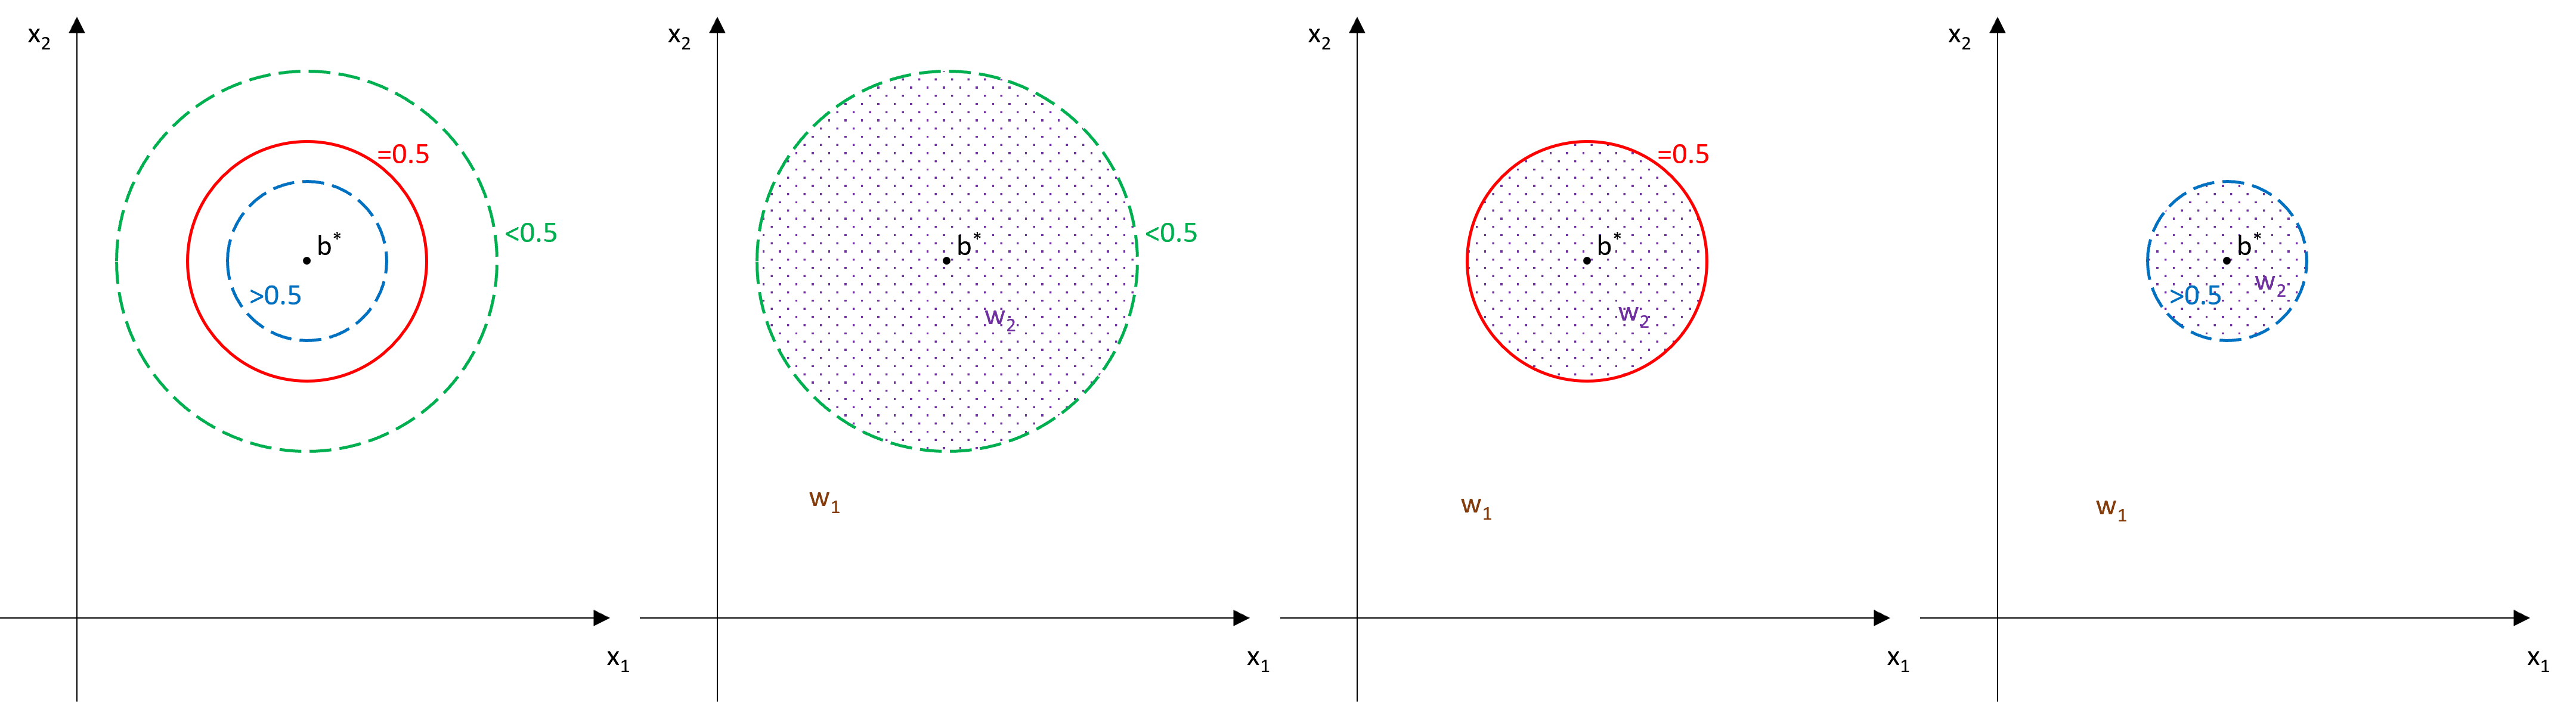
\includegraphics[scale=0.53]{C_4}
    \centering
\end{figure}
    \Exercise[number={5}]
A variable \(x\) in \(\mathbf{R}^2\) is emitted by two possible sources,
\(w_1\), \(w_2\) of probability \(Pr(w_1)=p\) and \(Pr(w_2)=1-p\). 
We want to design a Bayes classifier that assigns the correct class to each
observed \(x\). If the \(p(x|w_i)\) both have a Gaussian distribution, with
mean \(\mu_i\) and equal variances \(I\sigma^2\), show that for each \(p\)
the decision regions are bounded by a line perpendicular to the segment
\(\mu_1-\mu_2\).

\Answer[number={5}]
The boundaries of a binary classifier can be studied by computing the
sign of \(z(x)\), with \(z\) being the exponent of the sigmoid function, in
particular the decision boundaries are given by \(z(x)=0\).
\begin{align*}
    z(x)
    &=\log{\frac{p(x|w_1)}{p(x|w_2)}} + \log{\frac{Pr(w_1)}{Pr(w_2)}}
    =\log{p(x|w_1)}-\log{p(x|w_2)}+\log{\frac{p}{1-p}}\\
    &=-\cancel{\log{\frac{2\pi}{2\pi}}}-\cancel{\frac{1}{2}\log{\frac{|\Sigma_1|}{|\Sigma_2|}}}-\frac{1}{2\sigma^2}\bigl[(x-\mu_1)^T(x-\mu_1)-(x-\mu_2)^T(x-\mu_2)\bigr]+\log{\frac{p}{1-p}}\\
    &=-\frac{1}{2\sigma^2}\bigl[(\mu_1^T\mu_1-\mu_2^T\mu_2)-2(\mu_1-\mu_2)^Tx\bigr]+\log{\frac{p}{1-p}}\\
    &=-\frac{1}{2\sigma^2}\bigl[(\mu_1-\mu_2)^T(\mu_1+\mu_2-2x)\bigr]+\log{\frac{p}{1-p}}\\
    &=\frac{1}{\sigma^2}\biggl[(\mu_1-\mu_2)^T(x-\frac{\mu_1-\mu_2}{2})\biggr]+\log{\frac{p}{1-p}}
\end{align*}
\begin{align*}
    z(x)=0 \Longleftrightarrow \frac{1}{\sigma^2}\biggl[(\mu_1-\mu_2)^T(x-\frac{\mu_1-\mu_2}{2})\biggr]+\log{\frac{p}{1-p}}=0
\end{align*}
Notice that the first part of the equation is derived from
\(\log{\frac{p(x|w_1)}{p(x|w_2)}}\) and it must be zero on the decision
boundary, as both the likelihoods must be equal to 0.5. Moreover, it represents
a scalar product between two vectors: the first one represents the line
connecting \(\mu_1\) and \(\mu_2\), the second one is the line connecting
a generic \(x\) to the middle point of the line connecting the two means.
However, due to the presence of the right-side term \(\log{\frac{p}{1-p}}\),
the intersection point with the \(\mu_1-\mu_2\) line is moved from
the middle point towards the class center having a lower probability \(Pr(w_i)\),
making the area on the plane accounting for that lower probability class smaller.
In the 3D space, the equation \(z(x)=(\mu_1-\mu_2)^T(x-\frac{\mu_1-\mu_2}{2})\)
represents a hyperplane (in this case a plane), with an offset
\(\log{\frac{p}{1-p}}\), affecting where the plane intersects the plane
generated by \(x_1\) and \(x_2\) components.
Hence, three cases are possible:
\begin{enumerate}
    \item \(Pr(w_1)=Pr(w_2)=0.5\Rightarrow\log{\frac{p}{1-p}}=0\):
    the scalar product between the aforementioned vectors is null, implying
    that the two vectors must be perpendicular.
    \item \(Pr(w_1)=p>Pr(w_2)=1-p\Rightarrow\log{\frac{p}{1-p}}>0\):
    the scalar product must once again be zero, however, the factor
    \(\log{\frac{p}{1-p}}\) implies a translation of the decision line
    toward the \(\mu_2\) mean. This is consistent with a translation
    toward the negative side of the sigmoid, since there is a bias
    toward the selection of class \(w_1\) (\(Pr(w_1)>0.5\)).
    \item \(Pr(w_1)=p<Pr(w_2)=1-p\Rightarrow\log{\frac{p}{1-p}}<0\):
    the scalar product must once again be zero, however, the factor
    \(\log{\frac{p}{1-p}}\) implies a translation of the decision line
    toward the \(\mu_1\) mean. This is consistent with a translation
    toward the positive side of the sigmoid, since there is a bias
    toward the selection of class \(w_2\) (\(Pr(w_2)>0.5\)).
  \end{enumerate}
  A proof of the fact that all the three decision lines display the same
  slope (thus perpendicular to the \(\mu_1-\mu_2\) line) is given below:
  \begin{enumerate}
    \item \(Pr(w_1)=Pr(w_2)=0.5\Rightarrow\log{\frac{p}{1-p}}=0\):
    \begin{align*}
        z(x)=0
        &\Rightarrow
        (\mu_1-\mu_2)^T(x-\frac{\mu_1-\mu_2}{2})=0\\
        &\Rightarrow
        \begin{bmatrix}
            \mu_{1_{x_1}}-\mu_{2_{x_1}} && \mu_{1_{x_2}}-\mu_{2_{x_2}}
        \end{bmatrix}
        \begin{bmatrix}
            x_1-\frac{\mu_{1_{x_1}}-\mu_{2_{x_1}}}{2} \\ x_2-\frac{\mu_{1_{x_2}}-\mu_{2_{x_2}}}{2}
        \end{bmatrix}
        =0\\
        &\Rightarrow
        \begin{bmatrix}
            c_1 && c_2
        \end{bmatrix}
        \begin{bmatrix}
            x_1-\frac{c_1}{2} \\ x_2-\frac{c_2}{2}
        \end{bmatrix}
        =0\\
        &\Rightarrow
        c_1x_1-\frac{c_1^2}{2}+c_2x_2-\frac{c_2^2}{2}=0
        \Rightarrow
        x_2 = -\frac{c_1}{c_2}x_1+\frac{c_1^2+c_2^2}{2c_2}
    \end{align*}
    Therefore, the line slope is \(m=-\frac{c_1}{c_2}\).
    \item \(Pr(w_1)=p>Pr(w_2)=1-p\Rightarrow\log{\frac{p}{1-p}}>0\):
    \begin{align*}
        z(x)=0
        &\Rightarrow
        (\mu_1-\mu_2)^T(x-\frac{\mu_1-\mu_2}{2})+\log{\frac{p}{1-p}}=0\\
        &\Rightarrow
        \begin{bmatrix}
            \mu_{1_{x_1}}-\mu_{2_{x_1}} && \mu_{1_{x_2}}-\mu_{2_{x_2}}
        \end{bmatrix}
        \begin{bmatrix}
            x_1-\frac{\mu_{1_{x_1}}-\mu_{2_{x_1}}}{2} \\ x_2-\frac{\mu_{1_{x_2}}-\mu_{2_{x_2}}}{2}
        \end{bmatrix}
        =-\log{\frac{p}{1-p}}\\
        &\Rightarrow
        \begin{bmatrix}
            c_1 && c_2
        \end{bmatrix}
        \begin{bmatrix}
            x_1-\frac{c_1}{2} \\ x_2-\frac{c_2}{2}
        \end{bmatrix}
        =-\log{\frac{p}{1-p}}\\
        &\Rightarrow
        c_1x_1-\frac{c_1^2}{2}+c_2x_2-\frac{c_2^2}{2}=-\log{\frac{p}{1-p}}
        \Rightarrow
        x_2 = -\frac{c_1}{c_2}x_1+\frac{c_1^2+c_2^2}{2c_2}-\frac{1}{c_2}\log{\frac{p}{1-p}}
    \end{align*}
    Notice the line slope is still \(m=-\frac{c_1}{c_2}\), but the
    y-intercept has an additional term, shifting the
    decision boundary toward \(\mu_2\), the centre of class \(w_2\).
    \item \(Pr(w_1)=p<Pr(w_2)=1-p\Rightarrow\log{\frac{p}{1-p}}<0\):
    \begin{align*}
        z(x)=0
        &\Rightarrow
        (\mu_1-\mu_2)^T(x-\frac{\mu_1-\mu_2}{2})+\log{\frac{p}{1-p}}=0\\
        &\Rightarrow
        \begin{bmatrix}
            \mu_{1_{x_1}}-\mu_{2_{x_1}} && \mu_{1_{x_2}}-\mu_{2_{x_2}}
        \end{bmatrix}
        \begin{bmatrix}
            x_1-\frac{\mu_{1_{x_1}}-\mu_{2_{x_1}}}{2} \\ x_2-\frac{\mu_{1_{x_2}}-\mu_{2_{x_2}}}{2}
        \end{bmatrix}
        =-\log{\frac{p}{1-p}}\\
        &\Rightarrow
        \begin{bmatrix}
            c_1 && c_2
        \end{bmatrix}
        \begin{bmatrix}
            x_1-\frac{c_1}{2} \\ x_2-\frac{c_2}{2}
        \end{bmatrix}
        =-\log{\frac{p}{1-p}}\\
        &\Rightarrow
        c_1x_1-\frac{c_1^2}{2}+c_2x_2-\frac{c_2^2}{2}=-\log{\frac{p}{1-p}}
        \Rightarrow
        x_2 = -\frac{c_1}{c_2}x_1+\frac{c_1^2+c_2^2}{2c_2}-\frac{1}{c_2}\log{\frac{p}{1-p}}
    \end{align*}
    Also here the slope is \(m=-\frac{c_1}{c_2}\), but the
    y-intercept has an additional term of opposite sign w.r.t. the
    previous case, thus the decision boundary shifts toward
    \(\mu_1\), the centre of class \(w_1\).
  \end{enumerate}
    \Exercise[number={6}]
A variable \(x\) in \(\mathbf{R}^2\) is emitted by three possible sources,
\(w_1\), \(w_2\), \(w_3\) of probability \(Pr(w_1)=Pr(w_2)=Pr(w_3)\). 
All three \(p(x|w_i)\) have a Gaussian distribution, with
mean \(\mu_i\) and equal variances \(I\sigma^2\). We want to design a Bayes
classifier, which assigns the correct class to each observed \(x\).
Prove that the decision regions are delimited by the axes of the sides of the
triangle with vertices \(\mu_1\),\(\mu_2\), and \(\mu_3\) and in particular
pass through the center of the circumscribed circumference of the triangle
(circumcenter).

\Answer[number={6}]
It might be useful to study the decision boundaries between the three
couples of classes \(w_1\) and \(w_2\), \(w_2\) and \(w_3\), and
finally \(w_1\) and \(w_3\).\\
Let's start by deriving the first case (\(w_1\) and \(w_2\)):
\begin{align*}
    z(x)
    &=\log{\frac{p(x|w_1)}{p(x|w_2)}} + \cancel{\log{\frac{Pr(w_1)}{Pr(w_2)}}}
    =\log{p(x|w_1)}-\log{p(x|w_2)}\\
    &=-\cancel{\log{\frac{2\pi}{2\pi}}}-\cancel{\frac{1}{2}\log{\frac{|\Sigma_1|}{|\Sigma_2|}}}-\frac{1}{2\sigma^2}\bigl[(x-\mu_1)^T(x-\mu_1)-(x-\mu_2)^T(x-\mu_2)\bigr]\\
    &=-\frac{1}{2\sigma^2}\bigl[(\mu_1^T\mu_1-\mu_2^T\mu_2)-2(\mu_1-\mu_2)^Tx\bigr]\\
    &=-\frac{1}{2\sigma^2}\bigl[(\mu_1-\mu_2)^T(\mu_1+\mu_2-2x)\bigr]\\
    &=\frac{1}{\sigma^2}\biggl[(\mu_1-\mu_2)^T(x-\frac{\mu_1-\mu_2}{2})\biggr]
\end{align*}
\begin{align*}
    z(x)=0 \Longleftrightarrow \frac{1}{\sigma^2}\biggl[(\mu_1-\mu_2)^T(x-\frac{\mu_1-\mu_2}{2})\biggr]=0
\end{align*}
Once again, the decision boundary is given by the perpendicular bisector
of segment connecting \(\mu_1\) and \(\mu_2\).
A similar computation leads to the decision boundaries for the other two
cases, still the perpendicular bisectors for the segments connecting the
centers \(\mu_i\) of the selected classes.
Now, let's exploit the superimposition principle to combine the three
distinct decision boundaries:
\begin{figure}[H]
    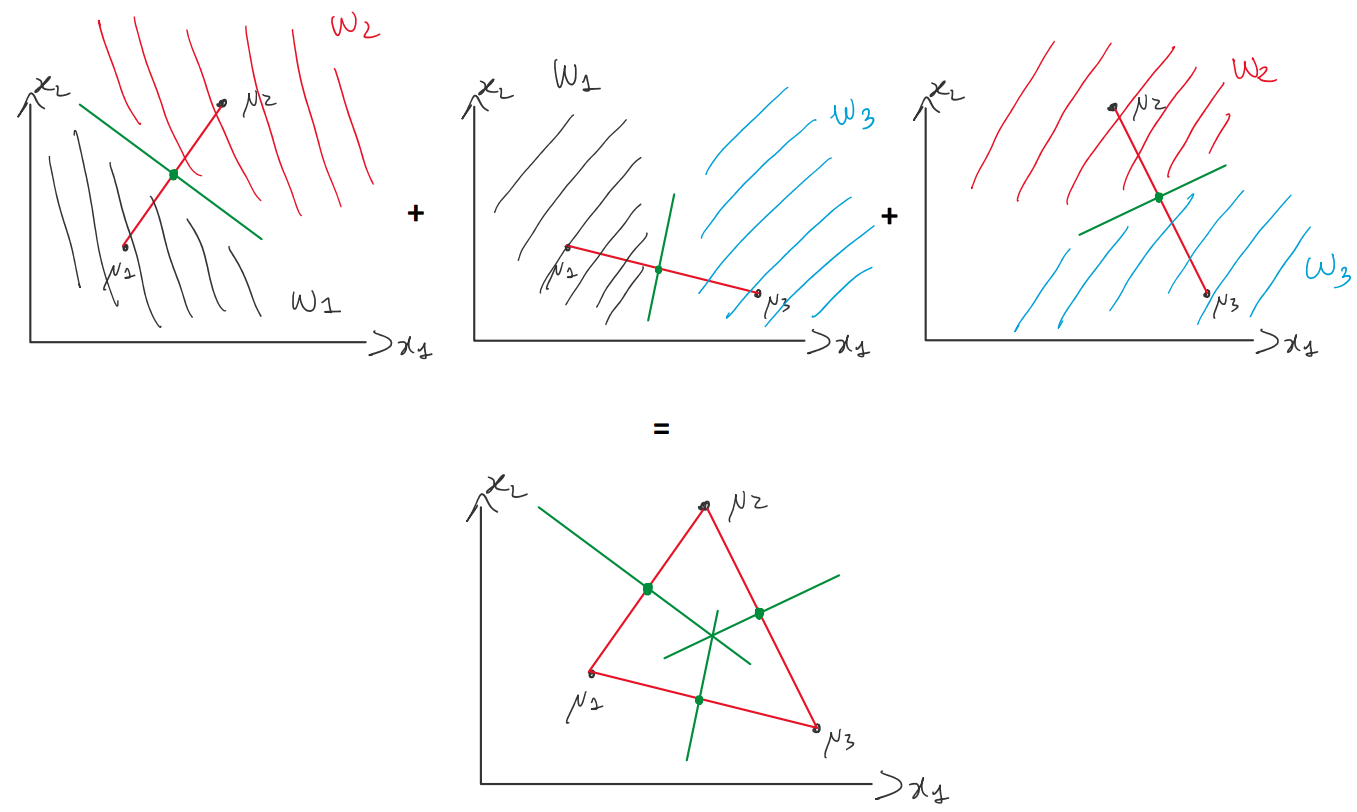
\includegraphics[scale=0.6]{C_6_1}
    \centering
\end{figure}
At this point, it is not difficult to state that the intersecting point
for the three decision boundaries must be the circumcenter for the
triangle defined by the vertices \(\mu_1\), \(\mu_2\) and \(\mu_3\),
as the three decision lines represent the perpendicular bisectors
for the triangle sides. Therefore, that point is coincident with the center
of the circumscribed circumference, by the definition of circumcenter.
\begin{figure}[H]
    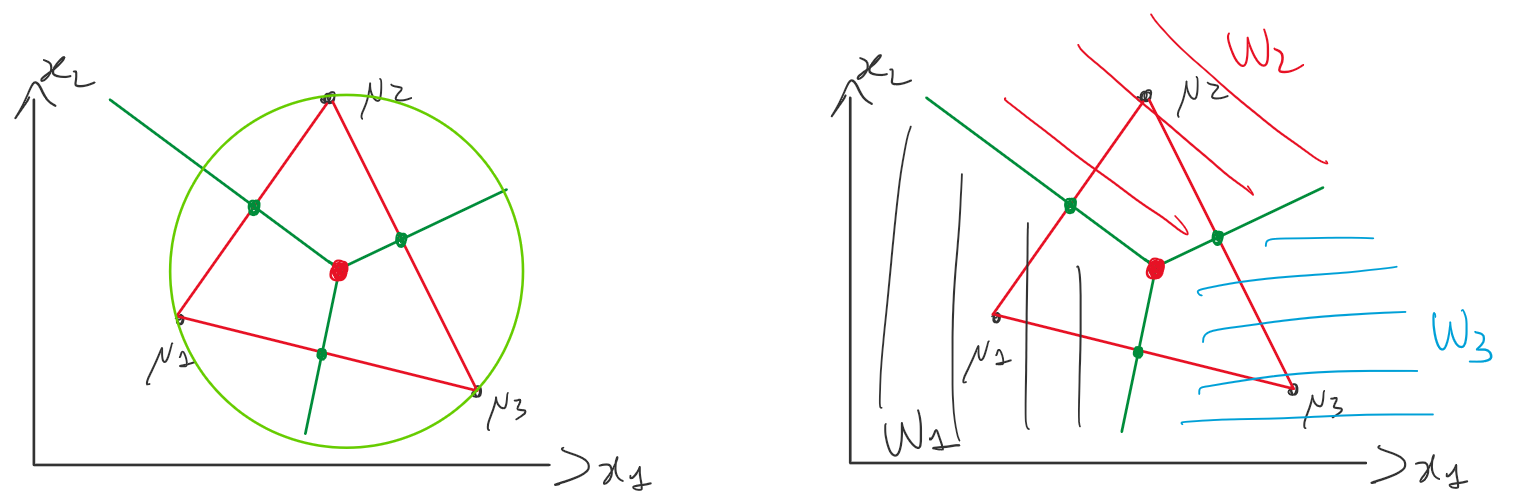
\includegraphics[scale=0.45]{C_6_2}
    \centering
\end{figure}
    \Exercise[number={7}]
We want to use a vector of measures \(x\) in \(\mathbf{R}^2\) to decide whether
an individual is affected \((w_1)\) or not \((w_2)\) by a given pathology.
The a priori probability that people of that age group and condition are
affected by the disease is \(Pr(w_1)=p\). We want to design a Bayes classifier
that attributes the correct class to each observed \(x\), while minimizing the
conditional risk. We know that the \(p(x|w_i)\) both have a Gaussian
distribution, with means \(\mu_i\) and equal variances \(I\sigma^2\).
However, the cost of the decision is asymmetric, in the sense that the cost of
the erroneous decision that the subject does not have the disease (false
negative) is \(h\) times greater (\(h>1\)) than the cost of erroneously
deciding that the subject has the disease (false positive). Correct decisions,
on the other hand, have a zero cost. Find the optimal classifier and discuss
how the decision regions vary as \(h\) varies.

\Answer[number={7}]
The two classes \(w_1\) and \(w_2\) can be denoted as \(P\) and \(N\)
respectively. Thus, the costs can be estimated as
\begin{align*}
    \begin{matrix}
        \lambda(P|P)=0 && \quad\quad\quad && \lambda(N|N)=0\\
        \lambda(N|P)=h && \quad\quad\quad && \lambda(P|N)=1
    \end{matrix}
\end{align*}
with \(h>1\).\\
Then the risk to detect a patient \(x\) as positive (class \(w_1=P\)) is
\begin{align*}
    R(P|x)
    =\cancel{\lambda(P|P)p(P|x)}+\lambda(P|N)p(N|x)
    =p(N|x)
\end{align*}
and the risk of a negtive detection (class \(w_2=N\)) is
\begin{align*}
    R(N|x)
    =\lambda(N|P)p(P|x)+\cancel{\lambda(N|N)p(N|x)}
    =h\cdot p(P|x)
\end{align*}
Notice that a person \(x\) will be classified as not affected (class \(N\))
if:
\begin{align*}
    R(N|x)<R(P|x)
    \Rightarrow h\cdot p(P|x)<p(N|x)
    \Rightarrow \frac{p(N|x)}{p(P|x)}>h
\end{align*}
If the logarithm is applied to both sides (monotonically increasing function):
\begin{align*}
    \log{\frac{p(N|x)}{p(P|x)}}>\log{h}
    \Rightarrow z(x)>\log{h}
\end{align*}
Therefore, the decision boundary is given by \(z(x)=\log{h}\):
\begin{align*}
    z(x)
    &=\log{\frac{p(N|x)}{p(P|x)}}
    =\log{\frac{p(x|N)Pr(N)}{p(x|P)Pr(P)}}\\
    &=\log{\frac{p(x|N)}{p(x|P)}} + \log{\frac{Pr(N)}{Pr(P)}}
    =\log{p(x|N)}-\log{p(x|P)}+\log{\frac{1-p}{p}}\\
    &=-\cancel{\log{\frac{2\pi}{2\pi}}}-\cancel{\frac{1}{2}\log{\frac{|\Sigma_1|}{|\Sigma_2|}}}-\frac{1}{2\sigma^2}\bigl[(x-\mu_1)^T(x-\mu_1)-(x-\mu_2)^T(x-\mu_2)\bigr]+\log{\frac{1-p}{p}}\\
    &=-\frac{1}{2\sigma^2}\bigl[(\mu_1^T\mu_1-\mu_2^T\mu_2)-2(\mu_1-\mu_2)^Tx\bigr]+\log{\frac{1-p}{p}}\\
    &=-\frac{1}{2\sigma^2}\bigl[(\mu_1-\mu_2)^T(\mu_1+\mu_2-2x)\bigr]+\log{\frac{1-p}{p}}\\
    &=\frac{1}{\sigma^2}\biggl[(\mu_1-\mu_2)^T(x-\frac{\mu_1-\mu_2}{2})\biggr]+\log{\frac{1-p}{p}}
\end{align*}
\begin{align*}
    z(x)=\log{h} \Longleftrightarrow \frac{1}{\sigma^2}\biggl[(\mu_1-\mu_2)^T(x-\frac{\mu_1-\mu_2}{2})\biggr]+\log{\frac{1-p}{p}}-\log{h}=0
\end{align*}
Let's highlight that
\(\log{\frac{1-p}{p}}-\log{h}=\log{\frac{1-p}{h\cdot p}}\), meaning that
the \(h\) term behaves in same way as the \(Pr(w_1)=Pr(P)=p\) bias.
Therefore, the cost \(h\) will move the decision boundary far from the
center of class \(w_1=P\), implying that classifying the person as negative
\(N\) is more difficult (as the risk of incurring in the \(h\) cost is
higher).
    \Exercise[number={8}]
Consider a one-dimensional binary decision problem, in which the conditional
densities are described by the Cauchy distribution:
\[
    p(x|w_i)=\frac{1}{\pi b}\frac{1}{1+\bigl(\frac{x-a_i}{b}\bigr)^2}
\]
Prove that if \(Pr(w_1)=Pr(w_2)\) the two posterior probabilities are equal
for \(x=(a_1+a_2)/2\).

\Answer[number={8}]
The decision criterion \(z(x)\) can be written as:
\begin{align*}
    z(x)
    &=\frac{\log{p(x|w_1)}}{\log{p(x|w_2)}}+\cancel{\log{\frac{Pr(w_1)}{Pr(w_2)}}}
    =\log{p(x|w_1)}-\log{p(x|w_2)}\\
    &=-\cancel{\log{\pi b}}-\log{\biggl[1+\biggl(\frac{x-a_1}{b}\biggr)^2\biggr]}+\cancel{\log{\pi b}}+\log{\biggl[1+\biggl(\frac{x-a_2}{b}\biggr)^2\biggr]}
\end{align*}
The decision boundary is obtained by setting \(z(x)\) equal to 0:
\begin{align*}
    z(x)=0
    &\Rightarrow
    -\log{\biggl[1+\biggl(\frac{x-a_1}{b}\biggr)^2\biggr]}+\log{\biggl[1+\biggl(\frac{x-a_2}{b}\biggr)^2\biggr]}=0\\
    &\Rightarrow
    \log{\biggl[1+\biggl(\frac{x-a_1}{b}\biggr)^2\biggr]}=\log{\biggl[1+\biggl(\frac{x-a_2}{b}\biggr)^2\biggr]}\\
    &\Rightarrow
    \cancel{1}+\biggl(\frac{x-a_1}{\cancel{b}}\biggr)^2=\cancel{1}+\biggl(\frac{x-a_2}{\cancel{b}}\biggr)^2\\
    &\Rightarrow
    \cancel{x^2}+a_1^2-2a_1x-\cancel{x^2}-a_2^2+2a_2x=0\\
    &\Rightarrow
    -2(a_1-a_2)x+(a_1^2-a_2^2)=0\\
    &\Rightarrow
    2\cancel{(a_1-a_2)}x=(a_1+a_2)\cancel{(a_1-a_2)}
    \Rightarrow
    x=\frac{a_1+a_2}{2}
\end{align*}
    \Exercise[number={9}]
Consider a one-dimensional binary decision problem, in which the conditional
densities are described by the Cauchy distribution:
\[
    p(x|w_i)=\frac{1}{\pi b}\frac{1}{1+\bigl(\frac{x-a_i}{b}\bigr)^2}
\]
Define a Bayesian classifier and determine the decision criterion,
assuming that \(Pr(w_1)=p\).\\
Draw \(p(w_1|x)\) and \(p(w_2|x)\) for \(a_1=3\), \(a_2=5\), \(b=1\),
\(p=0.5\).

\Answer[number={9}]
The decision criterion \(z(x)\) can be written as:
\begin{align*}
    z(x)
    &=\frac{\log{p(x|w_1)}}{\log{p(x|w_2)}}+\log{\frac{Pr(w_1)}{Pr(w_2)}}
    =\log{p(x|w_1)}-\log{p(x|w_2)}+\log{\frac{p}{1-p}}\\
    &=-\cancel{\log{\pi b}}-\log{\biggl[1+\biggl(\frac{x-a_1}{b}\biggr)^2\biggr]}+\cancel{\log{\pi b}}+\log{\biggl[1+\biggl(\frac{x-a_2}{b}\biggr)^2\biggr]}+\log{\frac{p}{1-p}}
\end{align*}
Then, the decision boundary for the given values is obtained by setting
\(z(x)\) equal to 0:
\begin{align*}
    z(x)=0
    &\Rightarrow
    -\log{\bigl[1+(x-3)^2\bigr]}+\log{\bigl[1+(x-5)^2\bigr]}+\cancel{\log{\frac{0.5}{0.5}}}=0\\
    &\Rightarrow
    \cancel{1}+(x-3)^2=\cancel{1}+(x-5)^2\\
    &\Rightarrow
    \cancel{x^2}+9-6x-\cancel{x^2}-25+10x=0\\
    &\Rightarrow
    4x=16
    \Rightarrow
    x=4
\end{align*}
Such a result is consistent with the general formula for \(Pr(w_1)=Pr(w_2)\),
stating that:
\begin{align*}
    x=\frac{a_1+a_2}{2}=\frac{3+5}{2}=\frac{8}{2}=4
\end{align*}
In order to estimate the posterior probabilities \(p(w_1|x)\) and \(p(w_2|x)\)
let's recall that:
\begin{align*}
    p(w_i|x)=\frac{1}{1+e^{-z_i(x)}}=\sigma_i(x)
    \quad\Longrightarrow\quad
    \text{sigmoid function}
\end{align*}
where
\begin{align*}
    z_1(x)=\log{\frac{1+(x-5)^2}{1+(x-3)^2}}
    \quad\text{and}\quad
    z_2(x)=\log{\frac{1+(x-3)^2}{1+(x-5)^2}}
\end{align*}
Let's study the function \(\sigma_1(x)=p(w_1|x)\):
\begin{itemize}
    \item\quad Domain: \(\mathfrak{D}=\mathbf{R}\)
    \item\quad Sign: \(\sigma_1(x)>0 \quad\forall{x}\in \mathbf{R}\)
    \item\quad Asymptotes:
    \begin{align*}
        \lim_{x\to{+\infty}}{\sigma_1(x)}=\frac{1}{2}
        \quad\text{and}\quad
        \lim_{x\to{-\infty}}{\sigma_1(x)}=\frac{1}{2}
    \end{align*}
    \item\quad Intersection with y-axis:
    \begin{align*}
        \sigma_1(0)
        =\frac{1}{1+e^{-\log{\frac{1+(0-5)^2}{1+(0-3)^2}}}}
        =\frac{1}{1+e^{-\log{\frac{26}{10}}}}
        =\frac{1}{1+\frac{26}{10}}
        =\frac{26}{36}
        \simeq 0.72
    \end{align*}
    \item\quad Decision criterion:
    \begin{align*}
        \sigma_1(x)=0.5
        \Rightarrow
        \frac{1}{1+\frac{x^2-6x+10}{x^2-10x+26}}=\frac{1}{2}
        \Rightarrow
        x=4
    \end{align*}
    \item\quad Maximum and minimum:
    \begin{align*}
        \sigma_1(x)
        =\frac{1}{1+e^{-\log{\frac{1+(x-5)^2}{1+(x-3)^2}}}}
        =\frac{x^2-10x+26}{2x^2-16x+36}
    \end{align*}
    \begin{align*}
        &\Rightarrow
        \frac{d\,\sigma_1(x)}{d\,x}
        =\frac{(2x-10)(2x^2-16x+36)-(x^2-10x+26)(4x-16)}{\cancel{(2x^2-16x+36)^2}}
        >0\\
        &\Rightarrow
        \cancel{4x^3}-20x^2-32x^2+\cancel{160x}+72x-360-\cancel{4x^3}+16x^2+40x^2-\cancel{160x}-104x+416>0\\
        &\Rightarrow
        x^2-8x+14>0\\
        &\Rightarrow
        x_{1,2}=4\pm\sqrt{16-14}=4\pm\sqrt{2}
    \end{align*}
    \(4-\sqrt{2}\quad\Rightarrow\quad\)maximum\(\quad\Rightarrow\quad\sigma_1(4-\sqrt{2})=0.854\)\\
    \(4+\sqrt{2}\quad\Rightarrow\quad\)minimum\(\quad\Rightarrow\quad\sigma_1(4+\sqrt{2})=0.146\)
\end{itemize}
The plot of \(\sigma_1(x)=p(w_1|x)\) is then:
\begin{figure}[H]
    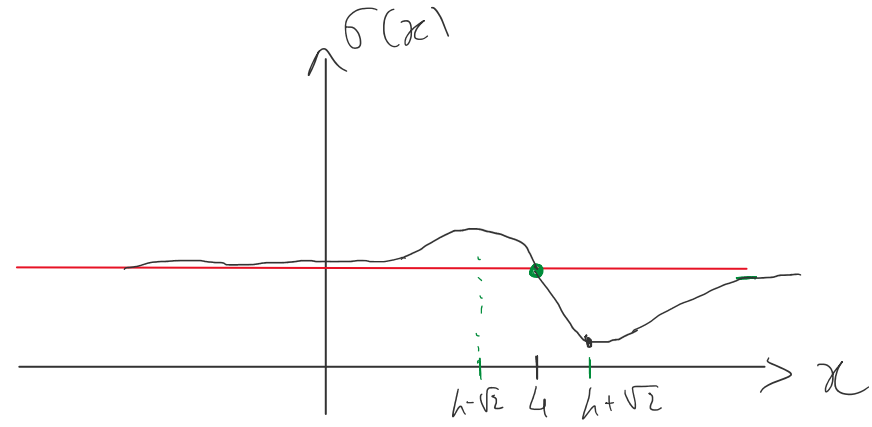
\includegraphics[scale=0.6]{C_9}
    \centering
\end{figure}
Notice that the plot of \(\sigma_2(x)=p(w_2|x)\) is symmetric to
\(\sigma_1(x)\) with respect to a symmetric axis defined as \(x=4\).
    \Exercise[number={10}]
Any binary classifier divides the \(x\) space into two regions,
\(\mathfrak{R}_1\) and \(\mathfrak{R}_2\). The probability of error is
defined by the sum of the propbability that the correct class is \(w_1\)
but \(x\) belongs to region \(\mathfrak{R}_2\) and the probability that
the correct class is \(w_2\) but \(x\) belongs to \(\mathfrak{R}_1\), i.e.
\(p(\text{error})=p(x\in\mathfrak{R}_2, w_1)+p(x\in\mathfrak{R}_1, w_2)\).
Suppose that \(x\) is defined in \(\mathbf{R}\) (scalar) and that both
\(p(x|w_i)\) have a Cauchy distribution:
\[
    p(x|w_i)=\frac{1}{\pi b}\frac{1}{1+\bigl(\frac{x-a_i}{b}\bigr)^2}
\]
with \(a_2>a_1\). Also assume that \(Pr(w_1)=Pr(w_2)=0.5\).\\
a. Define a Bayes classifier, and determine the decision regions.\\
b. Determine an expression for \(p(\text{error})\) as a function of
\(a_1\), \(a_2\), \(b\).\\
c. What happens to \(p(\text{error})\) when \((a_2-a_1)\to\infty\)?\\
\(\bigl[\)Hint: \(p(x\in\mathfrak{R}_2|w_1)=\int_{\mathfrak{R}_2}p(x|w_1)\,dx\)\(\bigr]\)

\Answer[number={10}]
a. The decision regions can be obtained as shown below:
\begin{align*}
    z(x)
    &=\frac{\log{p(x|w_1)}}{\log{p(x|w_2)}}+\cancel{\log{\frac{Pr(w_1)}{Pr(w_2)}}}
    =\log{p(x|w_1)}-\log{p(x|w_2)}\\
    &=-\cancel{\log{\pi b}}-\log{\biggl[1+\biggl(\frac{x-a_1}{b}\biggr)^2\biggr]}+\cancel{\log{\pi b}}+\log{\biggl[1+\biggl(\frac{x-a_2}{b}\biggr)^2\biggr]}
\end{align*}
\begin{align*}
    z(x)=0
    &\Rightarrow
    -\log{\biggl[1+\biggl(\frac{x-a_1}{b}\biggr)^2\biggr]}+\log{\biggl[1+\biggl(\frac{x-a_2}{b}\biggr)^2\biggr]}=0\\
    &\Rightarrow
    \cancel{1}+\biggl(\frac{x-a_1}{\cancel{b}}\biggr)^2=\cancel{1}+\biggl(\frac{x-a_2}{\cancel{b}}\biggr)^2\\
    &\Rightarrow
    \cancel{x^2}+a_1^2-2a_1x-\cancel{x^2}-a_2^2+2a_2x=0\\
    &\Rightarrow
    -2(a_1-a_2)x+(a_1^2-a_2^2)=0\\
    &\Rightarrow
    2\cancel{(a_1-a_2)}x=(a_1+a_2)\cancel{(a_1-a_2)}
    \Rightarrow
    x=\frac{a_1+a_2}{2}=x_b
\end{align*}
b. Notice that \(\mathfrak{R}_1=[-\infty; x_b]\) and
\(\mathfrak{R}_2=[x_b; +\infty]\).
Let's compute \(p(x\in\mathfrak{R}_2|w_1)\):
\begin{align*}
    p(x\in\mathfrak{R}_2|w_1)
    &=\int_{\mathfrak{R}_2}\frac{1}{\pi b}\frac{1}{1+\bigl(\frac{x-a_1}{b}\bigr)^2}\,dx\\
    &=\frac{1}{\pi b^2}\biggl[\arctan{t}\biggr]_{\mathfrak{R}_2}
    =\frac{1}{\pi b^2}\biggl[\arctan{\frac{x-a_1}{b}}\biggr]_{x_b}^{+\infty}
    \quad\quad\text{with } t=\frac{x-a_1}{b}\\
    &=\frac{1}{\pi b^2}\biggl(\frac{\pi}{2}-\arctan{\frac{\frac{a_1+a_2}{2}-a_1}{b}}\biggr)\\
    &=\frac{1}{2b^2}-\frac{1}{\pi b^2}\arctan{\frac{a_2-a_1}{2b}}
\end{align*}
Similarly,
\begin{align*}
    p(x\in\mathfrak{R}_1|w_2)
    &=\int_{\mathfrak{R}_1}\frac{1}{\pi b}\frac{1}{1+\bigl(\frac{x-a_2}{b}\bigr)^2}\,dx\\
    &=\frac{1}{\pi b^2}\biggl[\arctan{t}\biggr]_{\mathfrak{R}_1}
    =\frac{1}{\pi b^2}\biggl[\arctan{\frac{x-a_2}{b}}\biggr]_{-\infty}^{x_b}
    \quad\quad\text{with } t=\frac{x-a_2}{b}\\
    &=\frac{1}{\pi b^2}\biggl(\arctan{\frac{\frac{a_1+a_2}{2}-a_2}{b}+\frac{\pi}{2}}\biggr)\\
    &=\frac{1}{2b^2}-\frac{1}{\pi b^2}\arctan{\frac{a_2-a_1}{2b}}
\end{align*}
as \(\arctan\) is an odd function, thus \(\arctan(-x)=-\arctan(x)\).\\
Therefore,
\begin{align*}
    p(\text{error})
    &=p(x\in\mathfrak{R}_2, w_1)+p(x\in\mathfrak{R}_1, w_2)\\
    &=\frac{1}{2b^2}-\frac{1}{\pi b^2}\arctan{\frac{a_2-a_1}{2b}}+\frac{1}{2b^2}-\frac{1}{\pi b^2}\arctan{\frac{a_2-a_1}{2b}}\\
    &=\frac{1}{b^2}-\frac{2}{\pi b^2}\arctan{\frac{a_2-a_1}{2b}}
\end{align*}
c. As \((a_2-a_1)\to\infty\), the distance between the two distributions
increases, hence it is more and more difficult to have a significant
error, as the degree of overlapping of the two distributions decreases:
\begin{align*}
    \lim_{(a_2-a_1)\to\infty}p(\text{error})=\frac{1}{b^2}-\frac{\cancel{2}}{\cancel{\pi}b^2}\frac{\cancel{\pi}}{\cancel{2}}=0
\end{align*}
\begin{figure}[H]
    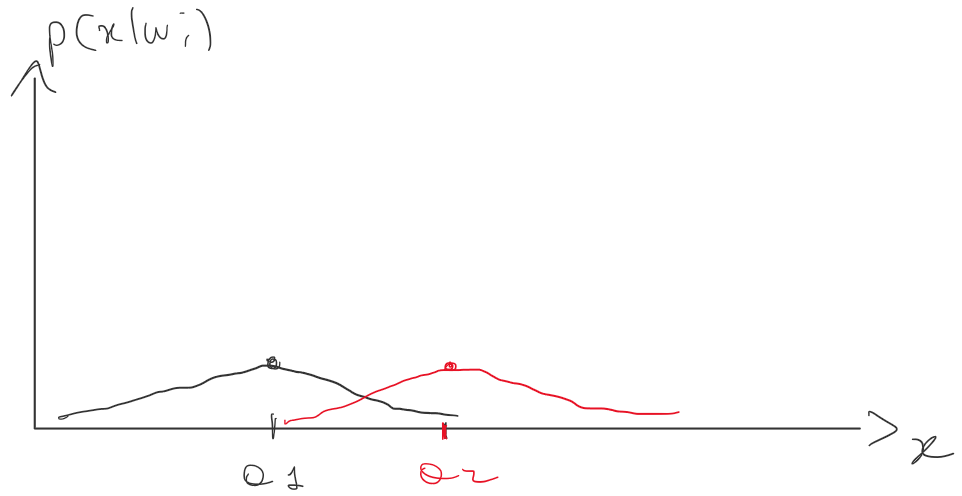
\includegraphics[scale=0.35]{C_10_1}
    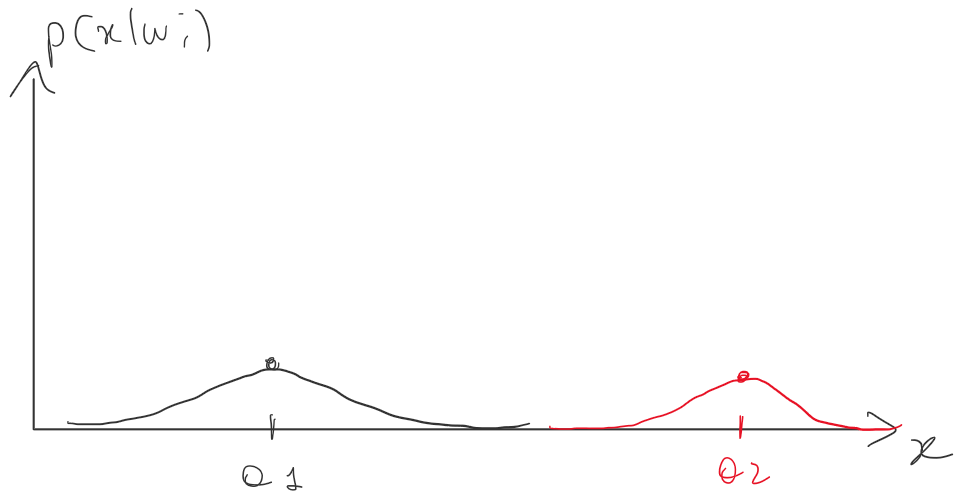
\includegraphics[scale=0.35]{C_10_2}
    \centering
\end{figure}
    \Exercise[number={11}]
Consider a vector of measures \(x=[x_1,...,x_d]^T\) in which each
component is statistically independent from the others and has binary
values (1 or 0). Consider 2 classes, with a-priori probabilities \(Pr(w_1)\)
and \(Pr(w_2)\). Let \(p(x_i=1|w_1)=p_i\) and \(p(x_i=1,w_2)=q_i\).
Find an expression for \(p(x|w_1)\) and \(p(x|w_2)\).\\
Finally, prove that the Bayesian decision rule is as follows:\\
Decide \(w_1\) if \(z(x)\ge 0\), where
\[
    z(x)=\sum_{i=1}^{d}x_i\log{\frac{p_i}{q_i}}+\sum_{i=1}^{d}(1-x_i)\log{\frac{1-p_i}{1-q_i}}+\log{\frac{Pr(w_1)}{Pr(w_2)}}
\]

\Answer[number={11}]
By recalling the Bernoulli distribution formula, the following likelihood
probabilities can be written:
\begin{align*}
    p(x|w_1)=\prod_{i=1}^{d}p_i^{x_i}(1-p_i)^{1-x_i}
    \quad\text{and}\quad
    p(x|w_2)=\prod_{i=1}^{d}q_i^{x_i}(1-q_i)^{1-x^i}
\end{align*}
The decision criterion \(z(x)\) is computed below:
\begin{align*}
    z(x)
    &=\log{\frac{p(x|w_1)}{p(x|w_2)}}+\log{\frac{Pr(w_1)}{Pr(w_2)}}
    =\log{p(x|w_1)}-\log{p(x|w_2)}+\log{\frac{Pr(w_1)}{Pr(w_2)}}\\
    &=\sum_{i=1}^{d}x_i\log{p_i}+\sum_{i=1}^{d}(1-x_i)\log{(1-p_i)}-\sum_{i=1}^{d}x_i\log{q_i}-\sum_{i=1}^{d}(1-x_i)\log{(1-q_i)}+\log{\frac{Pr(w_1)}{Pr(w_2)}}\\
    &=\sum_{i=1}^{d}x_i\log{\frac{p_i}{q_i}}+\sum_{i=1}^{d}(1-x_i)\log{\frac{1-p_i}{1-q_i}}+\log{\frac{Pr(w_1)}{Pr(w_2)}}
\end{align*}
This is exactly the expected expression.
    \Exercise[number={12}]
Two populations \(w_1\) and \(w_2\) of neurons emit spike trains. The
number \(n\) (integer) of spikes emitted during a certain observation
interval can be described for each of the two populations by a
class-conditioned Poisson type pdf:
\[
    p(n|w_i)=\frac{\lambda_i^n e^{-\lambda_i}}{n!}
\]
where \(\lambda_1\) and \(\lambda_2\) are different for the two
populations. We wanto to build a Bayes classifier that, starting from
the observation of a train of \(n\) spikes, decides from which of the
two populations of neurons it was generated.\\
Determine the boundaries of the decision regions and graphically
describe the result assuming \(\lambda_1>\lambda_2\).

\Answer[number={12}]
Let's write the decision criterion \(z(n)\) by assuming that
\(Pr(w_1)=Pr(w_2)\):
\begin{align*}
    z(n)
    &=\log{\frac{p(n|w_1)}{p(n|w_2)}}+\cancel{\log{\frac{Pr(w_1)}{Pr(w_2)}}}
    =\log{p(n|w_1)}-\log{p(n|w_2)}\\
    &=\log{\frac{\lambda_1^n e^{-\lambda_1}}{n!}}-\log{\frac{\lambda_2^n e^{-\lambda_2}}{n!}}
    =n\log{\lambda_1}-\lambda_1-\cancel{\log{n!}}-n\log{\lambda_2}+\lambda_2+\cancel{\log{n!}}\\
    &=n\log{\frac{\lambda_1}{\lambda_2}}-\lambda_1+\lambda_2
\end{align*}
Hence, the decision boundaries are obtained by setting \(z(n)\) equal to 0:
\begin{align*}
    z(n)=0
    \Longleftrightarrow
    n\log{\frac{\lambda_1}{\lambda_2}}-\lambda_1+\lambda_2=0
    \Rightarrow
    n=\frac{\lambda_1-\lambda_2}{\log{\frac{\lambda_1}{\lambda_2}}}
\end{align*}
Notice that \(\lambda_2<n<\lambda_1\) and that \(n\) is supposed to be an
integer, as the distributions are discrete. All the integers on the
left of \(n=\frac{\lambda_1-\lambda_2}{\log{\frac{\lambda_1}{\lambda_2}}}\)
are classified as class \(w_2\), the integer elements on the right as
class \(w_1\):
\begin{figure}[H]
    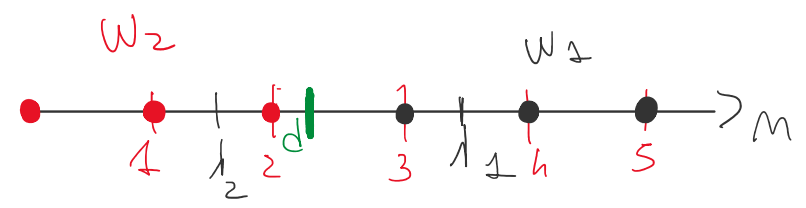
\includegraphics[scale=0.65]{C_12}
    \centering
\end{figure}
If the \(Pr(w_1)\neq{Pr(w_2)}\) assumption is done, then a more complex
expression for the decision boundaries is obtained:
\begin{align*}
    z(n)
    =\dots
    =n\log{\frac{\lambda_1}{\lambda_2}}-\lambda_1+\lambda_2+\log{\frac{Pr(w_1)}{Pr(w_2)}}
\end{align*}
\begin{align*}
    z(n)=0
    \Longleftrightarrow
    n\log{\frac{\lambda_1}{\lambda_2}}-\lambda_1+\lambda_2+\log{\frac{Pr(w_1)}{Pr(w_2)}}=0
    \Rightarrow
    n=\biggl[(\lambda_1-\lambda_2)-\log{\frac{Pr(w_1)}{Pr(w_2)}}\biggr]\frac{1}{\log{\frac{\lambda_1}{\lambda_2}}}
\end{align*}
    \Exercise[number={13}]
We intend to use a scalar measure \(x\) (scalar) to decide whether a
given individual is affected (\(w_1\)) or not (\(w_2\)) by a certain
pathology. Assume that the two classes have the same prior probability.
We know that \(x\) can only have three values: \(x\in\{0,1,2\}\) and that
for the two classes we respectively have:
\begin{align*}
    \begin{matrix}
        p(x=1|w_1)=q_{11} \\ p(x=1|w_2)=q_{12}
    \end{matrix}
    \text{ and }
    \begin{matrix}
        p(x=2|w_1)=q_{21} \\ p(x=2|w_2)=q_{22}
    \end{matrix}
    \quad
    \bigl[
        \text{How to compute }
        p(x=0|w_1)
        \text{ and }
        p(x=0|w_2)
        \text{?}
    \bigr]
\end{align*}
Design a Bayes classifier, which assigns the correct class to each
observed \(x\). Depending on the measured value of \(x\): 0 or 1 or 2,
specify (in terms of \(q_{11}\), \(q_{12}\), \(q_{21}\), \(q_{22}\)) the
relevant decision criterion.

\Answer[number={13}]
First of all, let's easily derive the following probabilities:
\begin{align*}
    p(x=0|w_1)=1-(q_{11}+q_{21})
    \quad\text{and}\quad
    p(x=0|w_2)=1-(q_{12}+q_{22})
\end{align*}
Now, the multi-class Bernoulli distribution is to be written, but first
it is necessary to compute the exponents. Let's denote
\(p_2(x)=ax^2+bx+c\) and then:
\begin{align*}
    \begin{cases}
        p_2(0)=0\\p_2(1)=1\\p_2(2)=0
    \end{cases}
    \Rightarrow
    \begin{cases}
        c=0\\a+b+c=1\\4a+2b+c=0
    \end{cases}
    \Rightarrow
    \begin{cases}
        c=0\\a=1-b\\4-4b+2b=0
    \end{cases}
    \Rightarrow
    \begin{cases}
        c=0\\a=-1\\b=2
    \end{cases}
\end{align*}
Therefore, the first exponent is given by \(p_2(x)=-x^2+2x=x(2-x)\).
\begin{align*}
    \begin{cases}
        p_2(0)=0\\p_2(1)=0\\p_2(2)=1
    \end{cases}
    \Rightarrow
    \begin{cases}
        c=0\\a+b+c=0\\4a+2b+c=1
    \end{cases}
    \Rightarrow
    \begin{cases}
        c=0\\a=-b\\-4b+2b=1
    \end{cases}
    \Rightarrow
    \begin{cases}
        c=0\\a=\frac{1}{2}\\b=-\frac{1}{2}
    \end{cases}
\end{align*}
The second exponent is \(p_2(x)=\frac{1}{2}x^2-\frac{1}{2}x=\frac{x}{2}(x-1)\).
\begin{align*}
    \begin{cases}
        p_2(0)=1\\p_2(1)=0\\p_2(2)=0
    \end{cases}
    \Rightarrow
    \begin{cases}
        c=1\\a+b+c=0\\4a+2b+c=0
    \end{cases}
    \Rightarrow
    \begin{cases}
        c=1\\a=-1-b\\-4-4b+2b+1=0
    \end{cases}
    \Rightarrow
    \begin{cases}
        c=1\\a=\frac{1}{2}\\b=-\frac{3}{2}
    \end{cases}
\end{align*}
Lastly, the third exponent is \(p_2(x)=\frac{1}{2}x^2-\frac{3}{2}x+1=\frac{1}{2}(x-1)(x-2)\).\\
Then, the multi-class Bernoulli distributions can be written as:
\begin{align*}
    p(x|w_1)
    &=q_{11}^{x(2-x)}\cdot q_{21}^{\frac{x}{2}(x-1)}\cdot\bigl[1-(q_{11}+q_{21})\bigr]^{\frac{1}{2}(1-x)(2-x)}\\
    p(x|w_2)
    &=q_{12}^{x(2-x)}\cdot q_{22}^{\frac{x}{2}(x-1)}\cdot\bigl[1-(q_{12}+q_{22})\bigr]^{\frac{1}{2}(1-x)(2-x)}
\end{align*}
Now it is easy to write down the decision criterion:
\begin{align*}
    z(x)
    &=\log{\frac{p(x|w_1)}{p(x|w_2)}}+\cancel{\log{\frac{Pr(w_1)}{Pr(w_2)}}}
    \log{p(x|w_1)}-\log{p(x|w_2)}\\
    &=x(2-x)\log{q_{11}}+\frac{x}{2}(x-1)\log{q_{21}}+\frac{1}{2}(1-x)(2-x)\log{\bigl[1-(q_{11}+q_{21})\bigr]}+\\
    &\quad-x(2-x)\log{q_{12}}-\frac{x}{2}(x-1)\log{q_{22}}-\frac{1}{2}(1-x)(2-x)\log{\bigl[1-(q_{12}+q_{22})\bigr]}\\
    &=x(2-x)\log{\frac{q_{11}}{q_{12}}}+\frac{x}{2}(x-1)\log{\frac{q_{21}}{q_{22}}}+\frac{1}{2}(1-x)(2-x)\log{\frac{1-(q_{11}+q_{21})}{1-(q_{12}+q_{22})}}
\end{align*}
Notice that if \(w_1\) is to be chosen, then \(z(x)>0\). Three cases
are possible:
\begin{enumerate}
    \item\quad \(x=1\Rightarrow z(x)=\log{\frac{q_{11}}{q_{12}}}>0\Longleftrightarrow q_{11}>q_{12}\)
    \item\quad \(x=2\Rightarrow z(x)=\log{\frac{q_{21}}{q_{22}}}>0\Longleftrightarrow q_{21}>q_{22}\)
    \item\quad \(x=0\Rightarrow z(x)=\log{\frac{1-(q_{11}+q_{21})}{1-(q_{12}+q_{22})}}>0\Longleftrightarrow \cancel{1}-(q_{11}+q_{21})>\cancel{1}-(q_{12}+q_{22})\Rightarrow q_{11}+q_{21}<q_{12}+q_{22}\)
\end{enumerate}
On the opposite, the \(w_2\) class is selected when \(z(x)<0\), thus
all the inequalities are inverted.
    \Exercise[number={14}]
A variable \(x\) in \(\mathbb{R}^2\) is emitted by two possible sources,
\(w_1\) and \(w_2\), with equal a-priori probabilities \(Pr(w_1)=Pr(w_2)\).
We want to design a Bayes classifier that assigns the correct class to
each observed \(x\). The \(p(x|w_i)\) both have a Gaussian distribution,
multivariate with means \(\mu_1\) and \(\mu_2\) and covariance
matrices \(\Sigma_1\) and \(\Sigma_2\).\\
a. Find an expression for the discriminant function \(z(x)\) in the
general case \(\mu_1\neq\mu_2\) and \(\Sigma_1\neq\Sigma_2\).\\
b. If \(\mu_1=(-a,0)\), \(\mu_2=(a,0)\), \(\Sigma_1=diag(1,2)\) and
\(\Sigma_2=diag(1,1)\) where \(a\) is a parameter, determine (for \(a>0\),
\(a<0\), and \(a=0\)) the locus of the points for which \(z(x)=0\).\\
c. Display graphically (under hypothesis b.) as accurately as possible
the contour of the decision regions.

\Answer[number={14}]
a. The discriminant function \(z(x)\) can be computed as follow:
\begin{align*}
    z(x)
    &=\log{\frac{p(x|w_1)}{p(x|w_2)}}+\cancel{\log{\frac{Pr(w_1)}{Pr(w_2)}}}
    =\log{p(x|w_1)}-\log{p(x|w_2)}\\
    &=-\frac{1}{2}\log{|\Sigma_1|}-\frac{1}{2}(x-\mu_1)^T\Sigma_1^{-1}(x-\mu_1)+\frac{1}{2}\log{|\Sigma_2|}+\frac{1}{2}(x-\mu_2)^T\Sigma_2^{-1}(x-\mu_2)\\
    &=\frac{1}{2}\log{\frac{|\Sigma_2|}{|\Sigma_1|}}-\frac{1}{2}(x-\mu_1)^T\Sigma_1^{-1}(x-\mu_1)+\frac{1}{2}(x-\mu_2)^T\Sigma_2^{-1}(x-\mu_2)
\end{align*}
b. Let's substitute the parameters' values into \(z(x)\):
\begin{align*}
    z(x)
    &=\frac{1}{2}\log{\frac{1}{2}}-\frac{1}{2}
    \begin{bmatrix}
        x_1+a && x_2
    \end{bmatrix}
    \begin{bmatrix}
        1 && 0 \\ 0 && \frac{1}{2}
    \end{bmatrix}
    \begin{bmatrix}
        x_1+a \\ x_2
    \end{bmatrix}
    +\frac{1}{2}
    \begin{bmatrix}
        x_1-a && x_2
    \end{bmatrix}
    \begin{bmatrix}
        1 && 0 \\ 0 && 1
    \end{bmatrix}
    \begin{bmatrix}
        x_1-a \\ x_2
    \end{bmatrix}\\
    &=-\frac{1}{2}\log{2}-\frac{1}{2}
    \begin{bmatrix}
        x_1+a && \frac{1}{2}x_2
    \end{bmatrix}
    \begin{bmatrix}
        x_1+a && x_2
    \end{bmatrix}
    +\frac{1}{2}
    \begin{bmatrix}
        x_1-a && x_2
    \end{bmatrix}
    \begin{bmatrix}
        x_1-a \\ x_2
    \end{bmatrix}\\
    &=-\frac{1}{2}\log{2}-\frac{1}{2}\bigl[(x_1+a)^2+\frac{1}{2}x_2^2\bigr]+\frac{1}{2}\bigl[(x_1-a)^2+x_2^2\bigr]\\
    &=-\frac{1}{2}\log{2}-\cancel{\frac{1}{2}x_1^2}-\cancel{\frac{1}{2}a^2}-ax_1-\frac{1}{4}x_2^2+\cancel{\frac{1}{2}x_1^2}+\cancel{\frac{1}{2}a^2}-ax_1+\frac{1}{2}x_2^2\\
    &=-\frac{1}{2}\log{2}-2ax_1+\frac{1}{4}x_2^2
\end{align*}
The decision boundary is obtained for \(z(x)=0\):
\begin{align*}
    z(x)=0
    \Longleftrightarrow
    -\frac{1}{2}\log{2}-2ax_1+\frac{1}{4}x_2^2=0
    \Rightarrow
    x_2^2=4(\frac{1}{2}\log{2}+2ax_1)
    \Rightarrow
    x_2=\pm\sqrt{4(\frac{1}{2}\log{2}+2ax_1)}
\end{align*}
Notice that for \(a=0\) the means of the two Gaussian distributions are
coincident, thus there is no decision boundary. While \(a>0\) the plot
on the left side is obtained, the one on the right side is instead
drawn for \(a<0\).
\begin{figure}[H]
    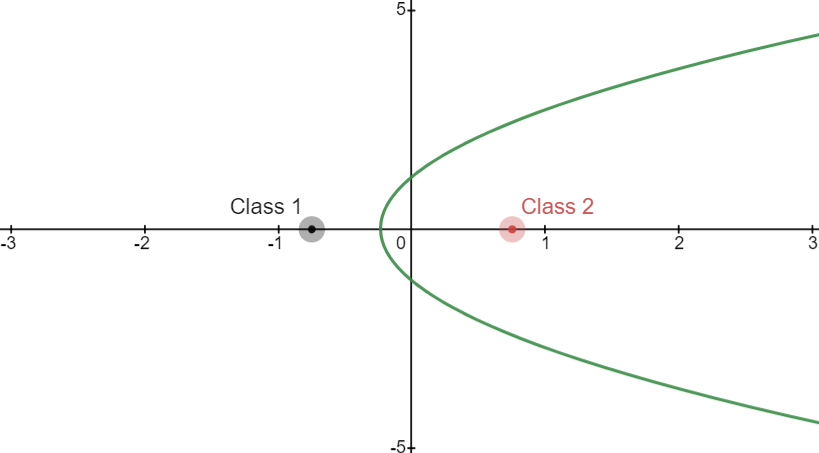
\includegraphics[scale=0.45]{C_14_1}
    \hspace{1cm}
    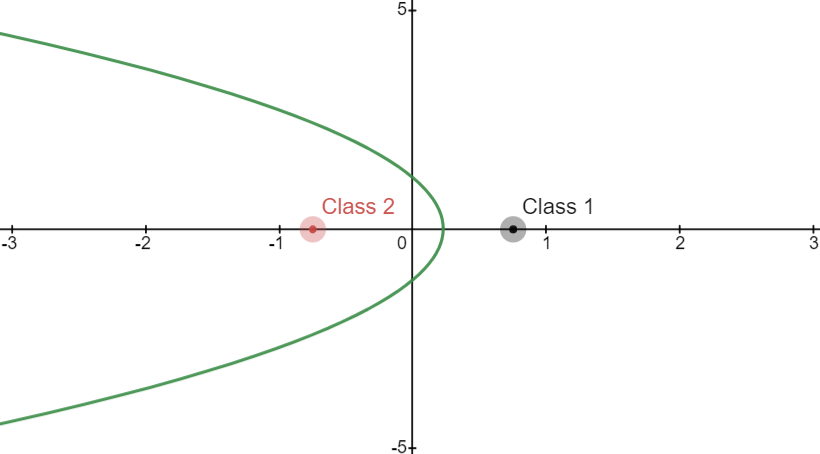
\includegraphics[scale=0.45]{C_14_2}
    \centering
\end{figure}
    \Exercise[number={15}]
In a binary classification problem, starting from a feature vector \(x\),
the linear discriminant vector \(w\) was obtained such that \(z=w^Tx\)
and the two classes in \(z\) are 'maximally separated' (linear
discriminant analysis, LDA). Suppose that a linear transformation is
applied to \(x: x'=Hx\) where \( H x\) is a diagonal matrix. Let \(w'\) be 
the discriminant vector for the new feature vector \(x'\).
What is the relationship between \(w\) and \(w'\)?

\Answer[number={15}]
TBD
    \Exercise[number={16}]
A generalized linear model is used to describe the relationship between a
feature vector \(x\) and an independent integer variable \(y\) that represents
the number of times an event occurs. The model is then defined by
\(z=b^T\cdot x\) where \(b\) is a vector of parameters, and \(y=f(z)\),
where \(f(...)\) is the output function. Prove that, if the observations
\(\hat{y}\) have a Poisson distribution, such as:
\begin{align*}
    p(\hat{y}|y)=\frac{e^{-y}\cdot y^{\hat{y}}}{\hat{y}!}
\end{align*}
then the canonical output function \(f(...)\) is the exponential.

\Answer[number={16}]
The drawing of the specified generalized linear model is the following one:
\begin{figure}[H]
    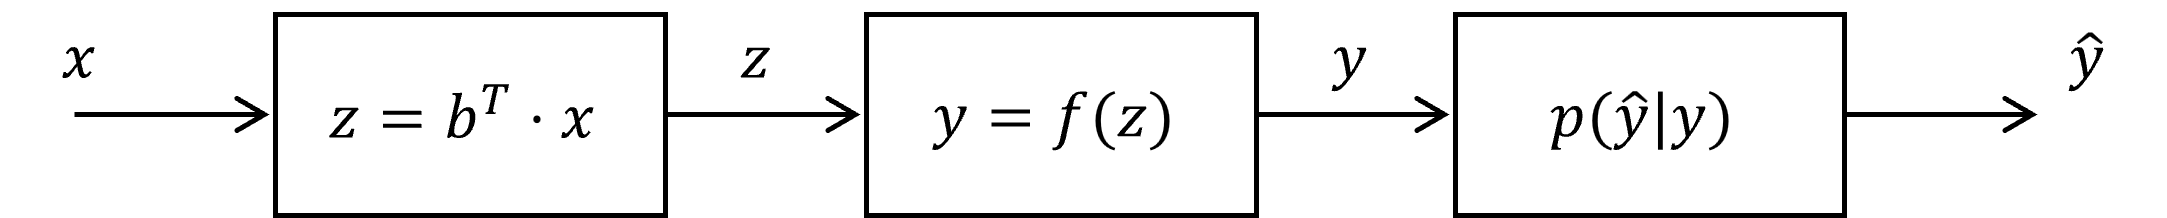
\includegraphics[scale=0.75]{C_16}
    \centering
\end{figure}
The dataset can be defined as \(D=\{(x_i, \hat{y_i}), i=1,...,N\}\), while
the likelihood is expressed as follow thanks to the chain rule:
\begin{align*}
    L(b|D)=L(b|(x_i, \hat{y}_i))
    =\prod_{i=1}^{N}p(x_i, \hat{y}_i|b)
    =\prod_{i=1}^{N}p(\hat{y}_i|x_i,b)p(x_i,b)
\end{align*}
Consequently, the log-likelihood is
\begin{align*}
    \log{L(b)}
    &=\sum_{i=1}^{N}\log{p(\hat{y}_i|x_i,b)}+\log{p(x_i)}
    =\sum_{i=1}^{N}\log{p(\hat{y}_i|y_i)}+\log{p(x_i)}\\
    &=\sum_{i=1}^{N}\biggl[\log{\frac{e^{-y_i}\cdot y_i^{\hat{y}_i}}{\hat{y}_i!}}\biggr]+constant\\
    &=\sum_{i=1}^{N}\biggl[\hat{y}_i\log{y_i}-y_i-\log{(\hat{y}_i!)}\biggr]+constant
\end{align*}
as \(y_i=f(z)=f(b^T\cdot x)\), moreover \(\log{p(x_i)}\) does not depend on
the parameter \(b\), meaning it is a constant.\\
Let's compute the derivative of the log-likelihood w.r.t. to the parameters
\(b\):
\begin{align*}
    \frac{\partial{\log{L(b)}}}{\partial{b}}
    &=\sum_{i=1}^{N}\biggl(\hat{y}_i\frac{1}{y_i}\frac{\partial{y_i}}{\partial{b}}-\frac{\partial{y_i}}{\partial{b}}\biggr)\\
    &=\sum_{i=1}^{N}\biggl(\frac{\hat{y}_i}{y_i}-1\biggr)\frac{\partial{y_i}}{\partial{b}}
    =\sum_{i=1}^{N}\biggl(\frac{\hat{y}_i}{y_i}-1\biggr)\frac{\partial{y_i}}{\partial{z_i}}\frac{\partial{z_i}}{\partial{b}}
    =\sum_{i=1}^{N}\biggl(\frac{\hat{y}_i}{y_i}-1\biggr)f'(z_i)\frac{\partial{z_i}}{\partial{b}}
\end{align*}
Notice that
\(\frac{\partial{z}}{\partial{b}}=\frac{\partial{b^T\cdot x}}{\partial{b}}=x\),
leading to:
\begin{align*}
    \frac{\partial{\log{L(b)}}}{\partial{b}}
    =\sum_{i=1}^{N}\biggl(\frac{\hat{y}_i}{y_i}-1\biggr)f'(z_i)x_i
    =\sum_{i=1}^{N}\biggl(\frac{\hat{y}_i-y_i}{y_i}\biggr)f'(z_i)x_i
\end{align*}
Since \(y=f(z)\), it can be said that:
\begin{align*}
    \frac{\partial{\log{L(b)}}}{\partial{b}}
    =\sum_{i=1}^{N}\biggl(\frac{\hat{y}_i-y_i}{f(z_i)}\biggr)f'(z_i)x_i
\end{align*}
However, an "error-like" function is to be obtained, looking similar to
\(\sum_{i=1}^{N}(\hat{y}_i-y_i)x_i\), thus a simplification as the following
one would be necessary:
\begin{align*}
    \frac{\partial{\log{L(b)}}}{\partial{b}}
    =\sum_{i=1}^{N}\biggl(\frac{\hat{y}_i-y_i}{\cancel{f(z_i)}}\biggr)\cancel{f'(z_i)}x_i
    =\sum_{i=1}^{N}(\hat{y}_i-y_i)x_i
\end{align*}
There is only one function such that \(f(z)=f'(z)\), henceforth the output
function must necessarily be \(f(z)=e^z\).

\end{ExerciseList}
\newpage

\section*{Unit D - Model selection}
\newpage

\section*{Unit E - Dynamic Models}
\graphicspath{ {./unit_E/images/} }
\begin{ExerciseList}
    \Exercise[number={1}]
Consider the following model, in which the discrete nodes \(S\) are binary,
while the continuous nodes, \(Y\), are Gaussian.
\begin{figure}[H]
    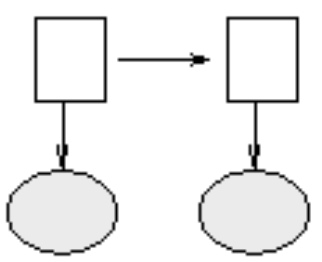
\includegraphics[scale=0.5]{E_1}
    \centering
\end{figure}
Define plausible expressions for the probabilities of initial, transition
and emission states, specifying their parameters. So suppose you have a
sequence \(Y=\{Y_1,...,Y_T\}\). Determine an expression for the likelihood
function:
\begin{align*}
    L(\theta)=p(S_{1:T}, Y_{1:T}|\theta)
\end{align*}

\Answer[number={1}]
Let's recall the HMM formula:
\begin{align*}
    Pr(S_{1:T}, y_{1:T}|\theta)
    &=Pr(S_1)\prod_{t=1}^{T}Pr(y_t|S_t)\prod_{t=2}^{T}Pr(S_t|S_{t-1})\\
    &=\text{initial state probability}\cdot\text{emission probability}\cdot\text{state transition probability}
\end{align*}
Notice that two states are available: \(s_1\) and \(s_2\). Moreover, the
probability that initial state \(S_1=s_1\) is \(\pi_1=p\), while the probability
that \(S_1=s_2\) is \(\pi_2=1-p\), leading to
\(\pi=[\pi_1\quad\pi_2]=[p\quad{1-p}]\).\\
Then, the initial state probability can be written as:
\begin{align*}
    P(S_1=s_i)
    =\prod_{i=1}^{2}\pi_i^{S_{1,i}}
    =\pi_1^{S_{1,1}}\cdot\pi_2^{S_{1,2}}
    =p^{S_{1,1}}\cdot(1-p)^{S_{1,2}}
\end{align*}
\begin{align*}
    \Rightarrow
    \log{Pr(S_1=s_i)}
    =\sum_{i=1}^{2}\log{\pi_i}^{S_{1,i}}
    =S_1^T\log{\pi}
\end{align*}
At this point, let's express the state transition probability as:
\begin{align*}
    Pr(S_t=s_t|S_{t-1}=s_{t-1})
    =\prod_{i=1}^2\prod_{j=1}^2(\phi_{ij})^{S_{t,i}\cdot S_{t-1,j}}
\end{align*}
\begin{align*}
    \Rightarrow
    \log{Pr(S_t=s_t|S_{t-1}=s_{t-1})}
    =\sum_{i=1}^2\sum_{j=1}^2S_{t,i}\cdot S_{t-1,j}\log{\phi_{ij}}
    =S_t^T\log{(\Phi)}S_{t-1}
\end{align*}
Finally, the emission probability can be written as follow, since the
observable nodes are Gaussian:
\begin{align*}
    p(y_t=y|S_t=s_i)
    =(2\pi)^{-\frac{d}{2}}|\Sigma|^{-\frac{1}{2}}\exp{\biggl\{-\frac{1}{2}(y_t-\mu)^T\Sigma^{-1}(y_t-\mu)\biggr\}}
\end{align*}
\begin{align*}
    \Rightarrow
    \log{p(y_t=y|S_t=s_i)}
    =-\frac{d}{2}\log{(2\pi)}-\frac{1}{2}\log{|\Sigma|}-\frac{1}{2}(y_t-\mu)^T\Sigma^{-1}(y_t-\mu)
\end{align*}
Henceforth:
\begin{align*}
    \log{Pr(S_{1:T}, y_{1:T}|\theta)}
    &=\log{Pr(S_1)}+\sum_{t=1}^{T}\log{Pr(y_t|S_t)}+\sum_{t=2}^{T}\log{Pr(S_t|S_{t-1})}\\
    &=S_1^T\log{\pi}+\sum_{t=1}^{T}\biggl[-\frac{d}{2}\log{(2\pi)}-\frac{1}{2}\log{|\Sigma|}-\frac{1}{2}(y_t-\mu)^T\Sigma^{-1}(y_t-\mu)\biggr]+\\
    &\quad +\sum_{t=2}^{T}S_t^T\log{(\Phi)}S_{t-1}
\end{align*}
    \Exercise[number={2}]
A virus exists in \(N\) different variants. At each generation the virus
mutates with probability \(0<p<1\) into a different variant, chosen at
random among the remaining ones. Calculate the probability that after \(n\) 
generations the virus type has not changed with respect to the initial
type (generation 1). 

\Answer[number={2}]
If \(p\) is the probability for a mutation to occur between two subsequent
generation, it is easy to see that the probability for a mutation not to
occur is just \(1-p\).\\
Said so, in order not to have a mutation between two generations:
\begin{align*}
    p(S_t|S_{t-1})=1-p
\end{align*}
By extending the formula to \(n\) generations one may simply obtain:
\begin{align*}
    p(S_n|S_{1:n-1})=\prod_{i=1}^{n}(1-p)=(1-p)^n
\end{align*}
    \Exercise[number={3}]
A trained mouse lives in the house depicted in the figure, consisting of
three interconnected rooms. A bell rings at regular intervals. The mouse is
trained to move into another room as soon as the bell rings.
When the mouse changes room, it chooses at random one of the available doors.
Mouse behavior can be represented as a Markov process in which the state
specifies the room \((A, B, C)\) where the mouse is located at a given time.
Determine the state transition matrix.
\begin{figure}[H]
    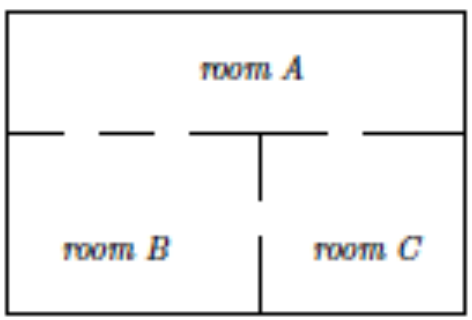
\includegraphics[scale=0.6]{E_2}
    \centering
\end{figure}

\Answer[number={3}]
The following probabilities can be obtained by simply counting the doors
available in each room, by assuming that the mouse cannot remain in the
same room for two subsequent intervals:
\begin{align*}
    \begin{matrix}
        S_{t-1}=A && S_{t-1}=B && S_{t-1}=C\\
        Pr(S_{t}=A|S_{t-1}=A)=0 && Pr(S_{t}=A|S_{t-1}=B)=\frac{2}{3} && Pr(S_{t}=A|S_{t-1}=C)=\frac{1}{2}\\
        Pr(S_{t}=B|S_{t-1}=A)=\frac{2}{3} && Pr(S_{t}=B|S_{t-1}=B)=0 && Pr(S_{t}=B|S_{t-1}=C)=\frac{1}{2}\\
        Pr(S_{t}=C|S_{t-1}=A)=\frac{1}{3} && Pr(S_{t}=C|S_{t-1}=B)=\frac{1}{3} && Pr(S_{t}=C|S_{t-1}=C)=0\\
    \end{matrix}
\end{align*}
As the state transition matrix is made of \(\phi_{ij}\) elements referred to
the \(i\)-th state \(S_{t}\) and \(j\)-th state \(S_{t-1}\), \(\Phi\) is:
\begin{align*}
    \Phi=
    \begin{bmatrix}
        \phi_{11} && \phi_{12} && \phi_{13}\\
        \phi_{21} && \phi_{22} && \phi_{23}\\
        \phi_{31} && \phi_{32} && \phi_{33}
    \end{bmatrix}
    =
    \begin{bmatrix}
        0 && \frac{2}{3} && \frac{1}{2}\\
        \frac{2}{3} && 0 && \frac{1}{2}\\
        \frac{1}{3} && \frac{1}{3} && 0
    \end{bmatrix}
\end{align*}
    \Exercise[number={4}]
Consider the following HMM:
\begin{figure}[H]
    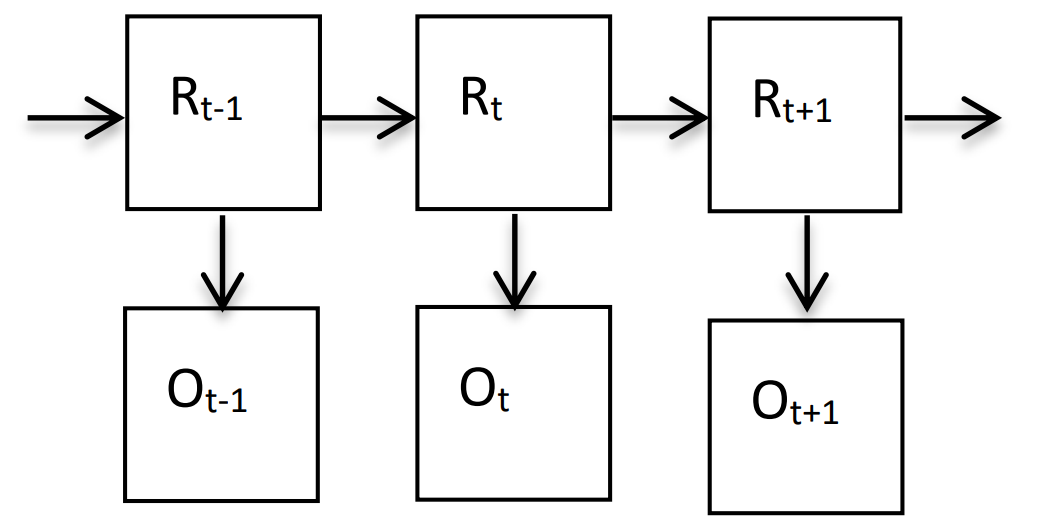
\includegraphics[scale=0.45]{E_3}
    \centering
\end{figure}
Which relates the observation that it rains on day (\(R_t=yes\))
with the observation that it has been raining the day before and that people
carry an umbrella, \(O_t = yes\).\\
You know that \(Pr(R_t=yes|R_{t-1}=yes)=0.8\) and that
\(Pr(R_t=yes|R_{t-1}=no)=0.1\). You also know that
\(Pr(O_t=yes|R_t=yes)=0.9\), \(Pr(O_t=yes|R_t=no)=0.3\) and
\(Pr(R_1=yes)=0.5\).\\
Calculate the probability to have rain on day 3 after having observed
people carrying umbrella (\(O_t=yes\)) for three consecutive days.

\Answer[number={4}]
First of all, let's compute explicitly all the necessary probabilities:
\begin{align*}
    \begin{matrix}
        Pr(R_1=yes)=0.5 && \Rightarrow && Pr(R_1=no)=1-0.5=0.5\\
        Pr(R_{t}=yes|R_{t-1}=yes)=0.8 && \Rightarrow && Pr(R_{t}=no|R_{t-1}=yes)=1-0.8=0.2\\
        Pr(R_{t}=yes|R_{t-1}=no)=0.1 && \Rightarrow && Pr(R_{t}=no|R_{t-1}=no)=1-0.1=0.9\\
        Pr(O_{t}=yes|R_{t}=yes)=0.9 && \Rightarrow && Pr(O_{t}=no|R_{t}=yes)=1-0.9=0.1\\
        Pr(O_{t}=yes|R_{t}=no)=0.3 && \Rightarrow && Pr(O_{t}=no|R_{t}=no)=1-0.3=0.7
    \end{matrix}
\end{align*}
The probability to have rain on day 3 after having observed
people carrying umbrella for three consecutive days can be summarized as:
\begin{align*}
    Pr(R_3=yes|O_{1:3}=yes)
    =Pr(R_3=yes|O_1=yes,O_2=yes,O_3=yes)
\end{align*}
In order to proceed, this conditional probability requires to be transformed
into a joint probability:
\begin{align*}
    Pr(R_3=yes|O_1=yes,O_2=yes,O_3=yes)
    =\frac{Pr(R_3=yes,O_1=yes,O_2=yes,O_3=yes)}{Pr(O_1=yes,O_2=yes,O_3=yes)}
\end{align*}
Now let's compute numerator (\(\mathcal{N}\)) and denominator (\(\mathcal{D}\)) values
separatelely. Let's start from the numerator:
\begin{align*}
    \mathcal{N}
    &=Pr(R_3=yes,O_1=yes,O_2=yes,O_3=yes)\\
    &=Pr(R_1,R_2,R_3=yes,O_1=yes,O_2=yes,O_3=yes)\\
    &=\sum_{R_1}\sum_{R_2}Pr(R_1)Pr(O_1=yes|R_1)Pr(R_2|R_1)Pr(O_2=yes|R_2)Pr(R_3=yes|R_2)Pr(O_3=yes|R_3=yes)
\end{align*}
\(R_1\) and \(R_2\) can assume two values each, meaning that there are
\(2^2=4\) possible combinations. Let's compute the respective probabilities:
\begin{align*}
    &1)R_1=yes, R_2=yes
    &\Rightarrow
    0.5\cdot0.9\cdot0.8\cdot0.9\cdot0.8\cdot0.9=0.23328\\
    &2)R_1=yes, R_2=no
    &\Rightarrow
    0.5\cdot0.9\cdot0.2\cdot0.3\cdot0.1\cdot0.9=0.00243\\
    &3)R_1=no, R_2=yes
    &\Rightarrow
    0.5\cdot0.3\cdot0.1\cdot0.9\cdot0.8\cdot0.9=0.00972\\
    &4)R_1=no, R_2=no
    &\Rightarrow
    0.5\cdot0.3\cdot0.9\cdot0.3\cdot0.1\cdot0.9=0.00365
\end{align*}
Therefore, \(\mathcal{N}=0.23328+0.00243+0.00972+0.00365\simeq0.2491\).\\
The denominator can be calculated by exploiting the same approach, however
\(R_3\) cannot be assumed always positive (as done in the numerator case),
in fact:
\begin{align*}
    \mathcal{D}
    &=Pr(O_1=yes,O_2=yes,O_3=yes)\\
    &=Pr(R_1,R_2,R_3,O_1=yes,O_2=yes,O_3=yes)\\
    &=Pr(R_1,R_2,R_3=yes,O_1=yes,O_2=yes,O_3=yes)+\\
    &\quad +Pr(R_1,R_2,R_3=no,O_1=yes,O_2=yes,O_3=yes)\\
    &=\mathcal{N}+Pr(R_1,R_2,R_3=no,O_1=yes,O_2=yes,O_3=yes)\\
    &=\mathcal{N}+\mathcal{D}'
\end{align*}
Let's now compute the part of the denominator accounting for \(R_3=no\):
\begin{align*}
    \mathcal{D}'
    &=Pr(R_1,R_2,R_3=no,O_1=yes,O_2=yes,O_3=yes)\\
    &=\sum_{R_1}\sum_{R_2}Pr(R_1)Pr(O_1=yes|R_1)Pr(R_2|R_1)Pr(O_2=yes|R_2)Pr(R_3=no|R_2)Pr(O_3=yes|R_3=no)
\end{align*}
Notice that if \(R_3\) is not known there are \(2^3=8\) possible cases, four
of them with \(R_3=yes\) (the ones computed in the numerator case) and four
with \(R_3=no\), which are to be computed below:
\begin{align*}
    &1)R_1=yes, R_2=yes
    &\Rightarrow
    0.5\cdot0.9\cdot0.8\cdot0.9\cdot0.2\cdot0.3=0.01944\\
    &2)R_1=yes, R_2=no
    &\Rightarrow
    0.5\cdot0.9\cdot0.2\cdot0.3\cdot0.9\cdot0.3=0.00729\\
    &3)R_1=no, R_2=yes
    &\Rightarrow
    0.5\cdot0.3\cdot0.1\cdot0.9\cdot0.2\cdot0.3=0.00081\\
    &4)R_1=no, R_2=no
    &\Rightarrow
    0.5\cdot0.3\cdot0.9\cdot0.3\cdot0.9\cdot0.3=0.01094
\end{align*}
Therefore, \(\mathcal{D}=\mathcal{N}+0.01944+0.00729+0.00081+0.01094=0.28758\).\\
Finally, \(Pr(R_3=yes|O_{1:3}=yes)=\frac{\mathcal{N}}{\mathcal{D}}=\frac{0.2491}{0.28758}=0.8662\simeq86.6\%\), a reasonable value.
    \Exercise[number={5}]
A doctor measures the value of a parameter \(P\) to monitor the evolution
of a patient's disease.\\
Parameter \(P\) can assume the values \(\{low, high\}\). The value of \(P\)
is the effect of a state or condition \(C\), not directly observable,
which can be \(\{good, bad\}\).
The status changes from one day to the next in \(1/5\) of cases. If the
patient is in a \(good\) condition, the \(P\) value is \(low\) on \(8/10\)
samples. If the patient is in as \(bad\) condition, the \(P\) value is
\(high\) on \(7/10\) samples. Upon arrival at the hospital (day 0), the
patient's condition is unknown, i.e. \(Pr(C=good)=0.5\).
\begin{itemize}
    \item\quad a. Formulate a model of the problem and draw the
    corresponding temporal model, specifying the corresponding probability
    table for each node.
    \item\quad b. Calculate the probability that the patient is in a
    \(good\) condition on day 2, given that \(P\) had a \(low\) value on
    day 1 and \(high\) on day 2.
\end{itemize}

\Answer[number={5}]
a. Here there is a schematization for the model:
\begin{figure}[H]
    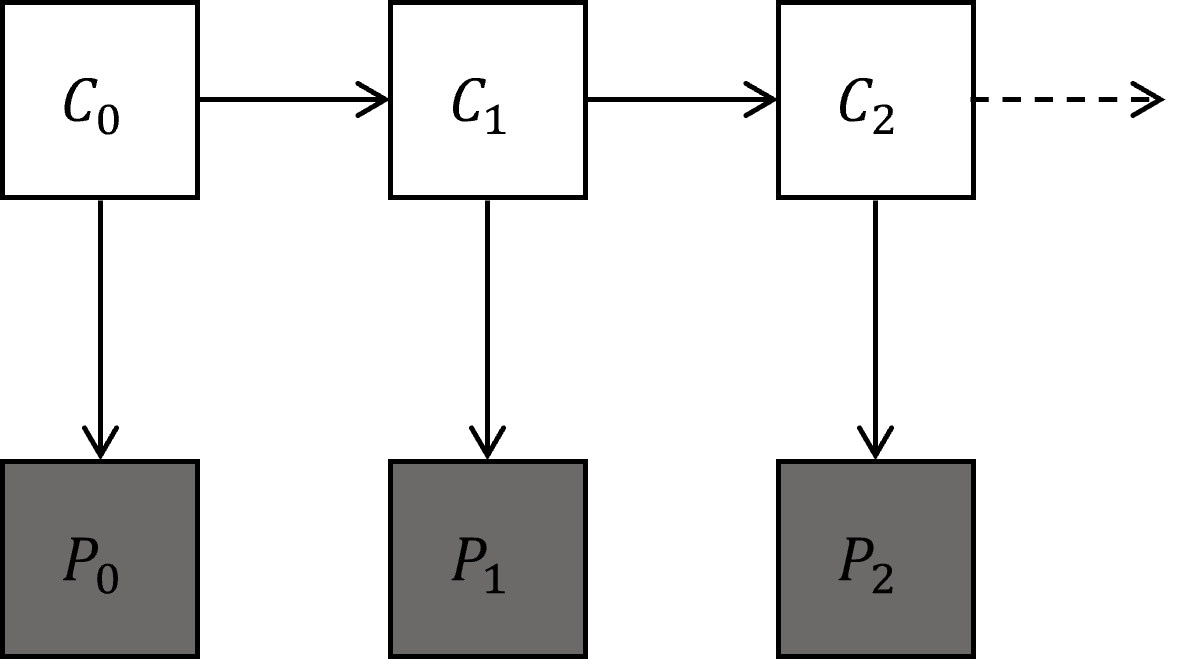
\includegraphics[scale=0.75]{E_5}
    \centering
\end{figure}
First of all, let's compute explicitly all the necessary probabilities:
\begin{align*}
    \begin{matrix}
        Pr(C_0=good)=0.5 && \Rightarrow && Pr(C_0=bad)=1-0.5=0.5\\
        Pr(C_{t}=good|C_{t-1}=bad)=0.2 && \Rightarrow && Pr(C_{t}=bad|C_{t-1}=bad)=1-0.2=0.8\\
        Pr(C_{t}=bad|C_{t-1}=good)=0.2 && \Rightarrow && Pr(C_{t}=good|C_{t-1}=good)=1-0.2=0.8\\
        Pr(P_{t}=low|C_{t}=good)=0.8 && \Rightarrow && Pr(P_{t}=high|C_{t}=good)=1-0.8=0.2\\
        Pr(P_{t}=high|C_{t}=bad)=0.7 && \Rightarrow && Pr(P_{t}=low|C_{t}=bad)=1-0.7=0.3
    \end{matrix}
\end{align*}
Then, the probability tables are:
\begin{align*}
    \begin{matrix}
        {} && C_0=good && C_0=bad\\
        Pr(C_0) && 0.5 && 0.5
    \end{matrix}
\end{align*}
\begin{align*}
    \begin{matrix}
        {} && C_t=good && C_t=bad\\
        Pr(C_t|C_{t-1}=good) && 0.8 && 0.2\\
        Pr(C_t|C_{t-1}=bad) && 0.2 && 0.8
    \end{matrix}
\end{align*}
\begin{align*}
    \begin{matrix}
        {} && P_t=low && P_t=high\\
        Pr(P_t|C_{t}=good) && 0.8 && 0.2\\
        Pr(P_t|C_{t}=bad) && 0.3 && 0.7
    \end{matrix}
\end{align*}
b. The probability that the patient is in a \(good\) condition on day 2,
given that \(P\) had a \(low\) value on day 1 and \(high\) on day 2 is:
\begin{align*}
    Pr(C_2=good|P_1=low,P_2=high)
    =Pr(C_2=good|C_0,C_1,P_0,P_1=low,P_2=high)
\end{align*}
In order to proceed, this conditional probability requires to be transformed
into a joint probability:
\begin{align*}
    Pr(C_2=good|P_1=low,P_2=high)
    =\frac{Pr(C_2=good,P_1=low,P_2=high)}{Pr(P_1=low,P_2=high)}
\end{align*}
Now let's compute numerator (\(\mathcal{N}\)) and denominator (\(\mathcal{D}\)) values
separatelely. Let's start from the numerator:
\begin{align*}
    \mathcal{N}
    &=Pr(C_2=good,P_1=low,P_2=high)\\
    &=Pr(C_0,C_1,C_2=good,P_0,P_1=low,P_2=high))\\
    &=\sum_{C_0}\sum_{C_1}\sum_{P_0}Pr(C_0)Pr(P_0|C_0)Pr(C_1|C_0)Pr(P_1=low|C_1)Pr(C_2=good|C_1)Pr(P_2=high|C_2=good)
\end{align*}
\(C_0\), \(C_1\) and \(P_0\) can assume two values each, meaning that there are
\(2^3=8\) possible combinations. Let's compute the respective probabilities:
\begin{align*}
    &1)C_0=good, C_1=good, P_0=low
    &\Rightarrow
    0.5\cdot0.8\cdot0.8\cdot0.8\cdot0.8\cdot0.2=0.04096\\
    &2)C_0=good, C_1=good, P_0=high
    &\Rightarrow
    0.5\cdot0.2\cdot0.8\cdot0.8\cdot0.8\cdot0.2=0.01024\\
    &3)C_0=good, C_1=bad, P_0=low
    &\Rightarrow
    0.5\cdot0.8\cdot0.2\cdot0.3\cdot0.2\cdot0.2=0.00096\\
    &4)C_0=good, C_1=bad, P_0=high
    &\Rightarrow
    0.5\cdot0.2\cdot0.2\cdot0.3\cdot0.2\cdot0.2=0.00024\\
    &5)C_0=bad, C_1=good, P_0=low
    &\Rightarrow
    0.5\cdot0.3\cdot0.2\cdot0.8\cdot0.8\cdot0.2=0.00384\\
    &6)C_0=bad, C_1=good, P_0=high
    &\Rightarrow
    0.5\cdot0.7\cdot0.2\cdot0.8\cdot0.8\cdot0.2=0.00896\\
    &7)C_0=bad, C_1=bad, P_0=low
    &\Rightarrow
    0.5\cdot0.3\cdot0.8\cdot0.3\cdot0.2\cdot0.2=0.00144\\
    &8)C_0=bad, C_1=bad, P_0=high
    &\Rightarrow
    0.5\cdot0.7\cdot0.2\cdot0.3\cdot0.2\cdot0.2=0.00084
\end{align*}
Therefore, \(\mathcal{N}=0.04096+...+0.00084\simeq0.01659\).\\
The denominator can be calculated by exploiting the same approach, however
\(C_2\) cannot be assumed always \(good\) (as done in the numerator case),
in fact:
\begin{align*}
    \mathcal{D}
    &=Pr(P_1=low,P_2=high)\\
    &=Pr(C_0,C_1,C_2,P_0,P_1=low,P_2=high)\\
    &=Pr(C_0,C_1,C_2=good,P_0,P_1=low,P_2=high)+\\
    &\quad +Pr(C_0,C_1,C_2=bad,P_0,P_1=low,P_2=high)\\
    &=\mathcal{N}+Pr(C_0,C_1,C_2=bad,P_0,P_1=low,P_2=high)\\
    &=\mathcal{N}+\mathcal{D}'
\end{align*}
Let's now compute the part of the denominator accounting for \(C_2=bad\):
\begin{align*}
    \mathcal{D}'
    &=Pr(C_0,C_1,C_2=bad,P_0,P_1=low,P_2=high)\\
    &=\sum_{C_0}\sum_{C_1}\sum_{P_0}Pr(C_0)Pr(P_0|C_0)Pr(C_1|C_0)Pr(P_1=low|C_1)Pr(C_2=bad|C_1)Pr(P_2=high|C_2=bad)
\end{align*}
Notice that if \(C_2\) is not known there are \(2^4=16\) possible cases, half
of them with \(C_2=good\) (the ones computed in the numerator case) and half
with \(C_2=bad\), which are to be computed below:
\begin{align*}
    &1)C_0=good, C_1=good, P_0=low
    &\Rightarrow
    0.5\cdot0.8\cdot0.8\cdot0.8\cdot0.2\cdot0.7=0.03584\\
    &2)C_0=good, C_1=good, P_0=high
    &\Rightarrow
    0.5\cdot0.2\cdot0.8\cdot0.8\cdot0.2\cdot0.7=0.00896\\
    &3)C_0=good, C_1=bad, P_0=low
    &\Rightarrow
    0.5\cdot0.8\cdot0.2\cdot0.3\cdot0.8\cdot0.7=0.01344\\
    &4)C_0=good, C_1=bad, P_0=high
    &\Rightarrow
    0.5\cdot0.2\cdot0.2\cdot0.3\cdot0.8\cdot0.7=0.00336\\
    &5)C_0=bad, C_1=good, P_0=low
    &\Rightarrow
    0.5\cdot0.3\cdot0.2\cdot0.8\cdot0.2\cdot0.7=0.00336\\
    &6)C_0=bad, C_1=good, P_0=high
    &\Rightarrow
    0.5\cdot0.7\cdot0.2\cdot0.8\cdot0.2\cdot0.7=0.00784\\
    &7)C_0=bad, C_1=bad, P_0=low
    &\Rightarrow
    0.5\cdot0.3\cdot0.8\cdot0.3\cdot0.8\cdot0.7=0.02016\\
    &8)C_0=bad, C_1=bad, P_0=high
    &\Rightarrow
    0.5\cdot0.7\cdot0.2\cdot0.3\cdot0.8\cdot0.7=0.01176
\end{align*}
Therefore, \(\mathcal{D}=\mathcal{N}+0.03584+...+0.01176=0.1722\).\\
Finally, \(Pr(C_2=good|P_1=low,P_2=high)=\frac{\mathcal{N}}{\mathcal{D}}=\frac{0.2491}{0.28758}=0.39187\simeq39.2\%\), a reasonable value.
    \Exercise[number={6}]
Consider the following linear dynamical system:
\begin{align*}
    \begin{cases}
        x_{i+1}=A\cdot x_i + w_i \\ y_i=C\cdot x_i + v_i
    \end{cases}
\end{align*}
where \(p(w_i)=\mathcal{N}(w_i|0,Q)\) and \(p(v_i)=\mathcal{N}(v_i|0,R)\).\\
Let \(A=[1\quad1; 0\quad1]\), \(C=[1\quad 1]\), \(R=\sigma_1^2\), \(Q=\sigma^2I_2\).\\
Also let (initial conditions): \(P_0^+=I_2\) and \(x_0^+=0\).
\begin{itemize}
    \item\quad a. Calculate \(K_1\) (Kalman gain at time \(i=1\)).
    \item\quad b. Calculate \(x_1^-\) and \(x_1^+\) (respectively, prior
    and posterior state estimate at time \(i=1\)) and the corresponding
    covariance matrices \(P_1^-\) and \(P_1^+\).
\end{itemize}

\Answer[number={6}]
a. First of all, let's recall the formulas to compute the Kalman gain and the
prior and posterior estimate for the state and for the variance:
\begin{align*}
    \begin{matrix}
        {} && K_t=\hat{P}_t^-C^T(C\hat{P}_t^-C^T+R)^{-1} && {}\\
        \hat{x}_t^-=A\hat{x}_{t-1}^+ && {} && \hat{x}_t^+=\hat{x}_t^-+K_t(y_t-C\hat{x}_t^-)\\
        \hat{P}_t^-=A\hat{P}_{t-1}^+A^T+Q && {} && \hat{P}_t^+=\hat{P}_t^--K_tC\hat{P}_t^-
    \end{matrix}
\end{align*}
In order to derive \(K_t\), \(P_1^-\) shall be computed:
\begin{align*}
    P_1^-
    =AP_0^+A^T+Q
    &=
    \begin{bmatrix}
        1&&1\\0&&1
    \end{bmatrix}
    \begin{bmatrix}
        1&&0\\0&&1
    \end{bmatrix}
    \begin{bmatrix}
        1&&0\\1&&1
    \end{bmatrix}
    +
    \begin{bmatrix}
        \sigma^2&&0\\0&&\sigma^2
    \end{bmatrix}\\
    &=
    \begin{bmatrix}
        1&&1\\0&&1
    \end{bmatrix}
    \begin{bmatrix}
        1&&0\\1&&1
    \end{bmatrix}
    +
    \begin{bmatrix}
        \sigma^2&&0\\0&&\sigma^2
    \end{bmatrix}
    =
    \begin{bmatrix}
        2&&1\\1&&1
    \end{bmatrix}
    +
    \begin{bmatrix}
        \sigma^2&&0\\0&&\sigma^2
    \end{bmatrix}\\
    &=
    \begin{bmatrix}
        2+\sigma^2&&1\\1&&1+\sigma^2
    \end{bmatrix}
\end{align*}
Therefore,
\begin{align*}
    K_1
    =\hat{P}_1^-C^T(C\hat{P}_1^-C^T+R)^{-1}
    &=
    \begin{bmatrix}
        2+\sigma^2&&1\\1&&1+\sigma^2
    \end{bmatrix}
    \begin{bmatrix}
        1\\1
    \end{bmatrix}
    \Biggl(
        \begin{bmatrix}
            1&&1
        \end{bmatrix}
        \begin{bmatrix}
            2+\sigma^2&&1\\1&&1+\sigma^2
        \end{bmatrix}
        \begin{bmatrix}
            1\\1
        \end{bmatrix}
        +\sigma_1^2
    \Biggr)^{-1}\\
    &=
    \begin{bmatrix}
        3+\sigma^2\\2+\sigma^2
    \end{bmatrix}
    \Biggl(
        \begin{bmatrix}
            3+\sigma^2&&2+\sigma^2
        \end{bmatrix}
        \begin{bmatrix}
            1\\1
        \end{bmatrix}
        +\sigma_1^2
    \Biggr)^{-1}\\
    &=
    \begin{bmatrix}
        3+\sigma^2\\2+\sigma^2
    \end{bmatrix}
    \biggl(
        5+2\sigma^2+\sigma_1^2
    \biggr)^{-1}
    =
    \frac{1}{5+2\sigma^2+\sigma_1^2}
    \begin{bmatrix}
        3+\sigma^2\\2+\sigma^2
    \end{bmatrix}
\end{align*}
b. Now, let's quickly compute
\begin{align*}
    \hat{x}_1^-=A\hat{x}_0^-=
    \begin{bmatrix}
        0\\0
    \end{bmatrix}
\end{align*}
while
\begin{align*}
    \hat{x}_1^+
    =\hat{x}_1^-+K_1(y_1-C\hat{x}_1^-)
    =\cancel{\hat{x}_1^-}+
    \frac{1}{5+2\sigma^2+\sigma_1^2}
    \begin{bmatrix}
        3+\sigma^2\\2+\sigma^2
    \end{bmatrix}
    \biggl(
        y_1-
        \cancel{
            \begin{bmatrix}
                1&&1
            \end{bmatrix}
            \hat{x}_1^-
        }
    \biggr)
    =\frac{y_1}{5+2\sigma^2+\sigma_1^2}
    \begin{bmatrix}
        3+\sigma^2\\2+\sigma^2
    \end{bmatrix}
\end{align*}
    \Exercise[number={7}]
Consider a LDS:
\begin{align*}
    \begin{matrix}
        x_{t+1}=Ax_t+Bu_t+w_t && p(w_t)=\mathcal{N}(w_t|0,Q)\\
        y_t=Cx_t+Du_t+v_t && p(v_t)=\mathcal{N}(v_t|0,R)
    \end{matrix}
\end{align*}
where \(u_t=a_t+n_t\) is an external input where \(a_t\) is observed
(i.e., known) whereas \(n_t\sim\mathcal{N}(0,D)\) (Gaussian noise with
covariance \(D\)). We intend to modify Kalman algorithm for the iterative
estimate of state \(x_t\) in order to also account for the input \(u_t\).
In particular:
\begin{itemize}
    \item\quad a. Modify the expression for the posterior state estimate.
    \item\quad b. Modify the corresponding iterative algorithm.
\end{itemize}

\Answer[number={7}]
TBD
    \Exercise[number={8}]
Consider the following linear dynamical system:
\begin{align*}
    \begin{cases}
        x_{i+1}=A\cdot x_i + w_i \\ y_i=C\cdot x_i + v_i
    \end{cases}
\end{align*}
where \(p(w_i)=\mathcal{N}(w_i|0,Q)\) and \(p(v_i)=\mathcal{N}(v_i|0,R)\).\\
Let \(A=I_2\) (identity 2x2 matrix), \(C=[1\quad1]\), \(R=\sigma_1^2\),
\(Q=\sigma^2I_2\).\\
Also let (initial conditions): \(P_0^+=I_2\) and \(x_0^+=0\).
\begin{itemize}
    \item\quad a. Calculate \(K_1\) (Kalman gain at time \(i=1\)).
    \item\quad b. Calculate \(x_1^+\) (posterior state estimate at
    time \(i=1\)).
\end{itemize}

\Answer[number={8}]
a. Let's recall the main formulas for the Kalman Filter:
\begin{align*}
    \begin{matrix}
        {} && K_t=\hat{P}_t^-C^T\bigl(C\hat{P}_t^-C^T+R\bigr)^{-1} && {}\\
        \hat{x}_t^-=A\hat{x}_{t-1}^+ && {} && \hat{x}_t^+=\hat{x}_t^-+K_t(y_t-C\hat{x}_t^-)\\
        \hat{P}_t^-=A\hat{P}_{t-1}^+A^T+Q && {} && \hat{P}_t^+=\hat{P}_t^--CK_t\hat{P}_t^-
    \end{matrix}
\end{align*}
Now the variance of the prior error can be computed:
\begin{align*}
    \hat{P}_1^-
    =A\hat{P}_{0}^+A^T+Q
    =I_2\cdot I_2\cdot I_2 + \sigma^2I_2
    =I_2+\sigma^2I_2
    =
    \begin{bmatrix}
        \sigma^2+1&&0\\0&&\sigma^2+1
    \end{bmatrix}
\end{align*}
Then, the Kalman gain is:
\begin{align*}
    K_1
    =\hat{P}_1^-C^T\bigl(C\hat{P}_1^-C^T+R\bigr)^{-1}
    &=
    \begin{bmatrix}
        \sigma^2+1&&0\\0&&\sigma^2+1
    \end{bmatrix}
    \begin{bmatrix}
        1\\1
    \end{bmatrix}
    \Biggl(
        \begin{bmatrix}
            1&&1
        \end{bmatrix}
        \begin{bmatrix}
            \sigma^2+1&&0\\0&&\sigma^2+1
        \end{bmatrix}
        \begin{bmatrix}
            1\\1
        \end{bmatrix}
        +\sigma_1^2
    \Biggr)^{-1}\\
    &=
    \begin{bmatrix}
        \sigma^2+1\\\sigma^2+1
    \end{bmatrix}
    \Biggl(
        \begin{bmatrix}
            1&&1
        \end{bmatrix}
        \begin{bmatrix}
            \sigma^2+1\\\sigma^2+1
        \end{bmatrix}
        +\sigma_1^2
    \Biggr)^{-1}\\
    &=
    \begin{bmatrix}
        \sigma^2+1\\\sigma^2+1
    \end{bmatrix}
    \bigl(2\sigma^2+2+\sigma_1^2\bigr)^{-1}
    =
    \frac{1}{2\sigma^2+2+\sigma_1^2}
    \begin{bmatrix}
        \sigma^2+1\\\sigma^2+1
    \end{bmatrix}
\end{align*}
b. The prior state estimate is to be computed as follow:
\begin{align*}
    \hat{x}_1^-
    =A\hat{x}_0^+
    =
    \begin{bmatrix}
        1&&1
    \end{bmatrix}
    \begin{bmatrix}
        0\\0
    \end{bmatrix}
    =
    \begin{bmatrix}
        0\\0
    \end{bmatrix}
\end{align*}
Therefore, the posterior state estimate at \(t=1\) is expressed as:
\begin{align*}
    \hat{x}_1^+
    =\cancel{\hat{x}_1^-}+K_1(y_1-\cancel{C\hat{x}_1^-})
    =K_1y_1
    =
    \frac{y_1}{2\sigma^2+2+\sigma_1^2}
    \begin{bmatrix}
        \sigma^2+1\\\sigma^2+1
    \end{bmatrix}
\end{align*}
\end{ExerciseList}
\newpage

\section*{Unit F - System identification}
\graphicspath{ {./unit_F/images/} }
\begin{ExerciseList}
    \Exercise[number={1}]
Find the optimal predictor, \(\hat{y}(t|t-1,\theta)\) for the following
system assuming \(E\{e(t)\}=0\) and \(E\{e(t)e(s)\}=\lambda^2\delta(t-s)\)
(notice that \(y(t|t-1,\theta)\) is a function of \(\{(u(s),y(s))\}_{s<t}\)).\\
The system is:
\begin{align*}
    y(t)=e(t)
\end{align*}

\Answer[number={1}]
From the general formula of a dynamic system, the \(G\) and \(H\)
parameters can be derived as follow:
\begin{align*}
    y(t)=Gu(t)+He(t)=e(t)
    \Rightarrow
    G=0 \quad\text{and}\quad H=1
\end{align*}
Therefore, the optimal predictor is easily obtained:
\begin{align*}
    \hat{y}(t|t-1,\theta) = (1-H^{-1})y(t)+H^{-1}Gu(t)
    \Rightarrow
    \hat{y}(t|t-1,\theta) = 0y(t)+0u(t)=0
\end{align*}
    \Exercise[number={2}]
Find the optimal predictor, \(\hat{y}(t|t-1,\theta)\) for the following
system assuming \(E\{e(t)\}=0\) and \(E\{e(t)e(s)\}=\lambda^2\delta(t-s)\)
(notice that \(y(t|t-1,\theta)\) is a function of \(\{(u(s),y(s))\}_{s<t}\)).\\
The system is:
\begin{align*}
    (1-0.1q^{-1})y(t)=-0.5q^{-1}u(t)+e(t)
\end{align*}

\Answer[number={2}]
From the general formula of a dynamic system, the \(G\) and \(H\)
parameters can be derived as follow:
\begin{align*}
    y(t)=Gu(t)+He(t)
    \Rightarrow
    G=\frac{-0.5q^{-1}}{1-0.1q^{-1}} \quad\text{and}\quad H=\frac{1}{1-0.1q^{-1}}
\end{align*}
Therefore, the optimal predictor is defined as
\begin{align*}
    \hat{y}(t|t-1,\theta) = L_1y(t)+L_2u(t) = (1-H^{-1})y(t)+H^{-1}Gu(t)
\end{align*}
and the parameters \(L_1\) and \(L_2\) are easily computed below:
\begin{align*}
    &\Rightarrow
    L_1 = 1-H^{-1} = 1-(1-0.1q^{-1}) = 0.1q^{-1}\\
    &\Rightarrow
    L_2 = H^{-1}G = \cancel{(1-0.1q^{-1})}\frac{-0.5q^{-1}}{\cancel{1-0.1q^{-1}}}=-0.5q^{-1}
\end{align*}
Leading to the optimal predictor:
\begin{align*}
    \hat{y}(t|t-1,\theta) = 0.1q^{-1}y(t)-0.5q^{-1}u(t)
\end{align*}
Notice that the considered dynamical system is an ARX model.
    \Exercise[number={3}]
Find the optimal predictor, \(\hat{y}(t|t-1,\theta)\) for the following
system assuming \(E\{e(t)\}=0\) and \(E\{e(t)e(s)\}=\lambda^2\delta(t-s)\)
(notice that \(y(t|t-1,\theta)\) is a function of \(\{(u(s),y(s))\}_{s<t}\)).\\
The system is:
\begin{align*}
    (1-0.1q^{-1})y(t)=-0.5q^{-1}u(t)+(1-0.8q^{-1})e(t)
\end{align*}

\Answer[number={3}]
From the general formula of a dynamic system, the \(G\) and \(H\)
parameters can be derived as follow:
\begin{align*}
    y(t)=Gu(t)+He(t)
    \Rightarrow
    G=\frac{-0.5q^{-1}}{1-0.1q^{-1}} \quad\text{and}\quad H=\frac{1-0.8q^{-1}}{1-0.1q^{-1}}
\end{align*}
Therefore, the optimal predictor is defined as
\begin{align*}
    \hat{y}(t|t-1,\theta) = L_1y(t)+L_2u(t) = (1-H^{-1})y(t)+H^{-1}Gu(t)
\end{align*}
and the parameters \(L_1\) and \(L_2\) are easily computed below:
\begin{align*}
    &\Rightarrow
    L_1 = 1-H^{-1} = 1-\frac{1-0.1q^{-1}}{1-0.8q^{-1}} = \frac{\cancel{1}-0.8q^{-1}-\cancel{1}+0.1q^{-1}}{1-0.8q^{-1}}=\frac{-0.7q^{-1}}{1-0.8q^{-1}}\\
    &\Rightarrow
    L_2 = H^{-1}G = \frac{\cancel{1-0.1q^{-1}}}{1-0.8q^{-1}}\frac{-0.5q^{-1}}{\cancel{1-0.1q^{-1}}}=\frac{-0.5q^{-1}}{1-0.8q^{-1}}
\end{align*}
Leading to the optimal predictor:
\begin{align*}
    \hat{y}(t|t-1,\theta) = \frac{-0.7q^{-1}}{1-0.8q^{-1}}y(t)-\frac{0.5q^{-1}}{1-0.8q^{-1}}u(t)
\end{align*}
Notice that the considered dynamical system is an ARMAX model.
\end{ExerciseList}   
\end{document}